\documentclass[master=cws, masteroption=vs]{kulemt}

% Vul de titel van jouw masterproef hieronder in tussen { en }.

\setup{title={Flip the virus:  Modelling targeted attacks using FlipIt with propagation delay},
%
% Vul hieronder namen in, steeds Voornaam Naam.
% Indien meerdere auteurs, assessoren, assistenten, scheidt hun namen
% met \and .
author={Sophie Marien},
promotor={Prof. dr. T. Holvoet},
assessor={Prof. dr. B. Jacobs \and Dr. ir. A. Dries},
assistant={Ir. Jonathan Merlevede, \and Ir. Kristof Coninx}}
% 
% De volgende \setup mag verwijderd worden als geen fiche gewenst is.
\setup{filingcard,
  translatedtitle={Flip the virus:  Modelling targeted attacks using FlipIt with propagation delay},
  udc=621.3,
  shortabstract={Recently, high profile targeted attacks such as the
attack on Belgacom (a major Belgian telcom), have demonstrated
that even the most secure companies can still be compromised,
and that moreover such attacks can go undetected for a while. These kind of attacks are called APT, advanced persistent threats, which are designed to penetrate secretly a computer network, collect sensitive data and stay hidden for many years. A company has every interest to mitigate the risks of an APT and the consequences that it can cause.  Because of the stealthiness fighting against these attacks requires methods that go beyond the standard tools against malware.
A group of researchers at the RSA, van Dijk et al., proposed the game FlipIt (The game of ``stealthy takeover'') to model stealthy takeovers. It is a 2-players game composed of
a single attacker, a single defender and a single shared resource.
The players will 
compete to get control over the shared resource. Every move of the players will involve a cost and
these moves happen in a stealthy way. The objective of the game for each player is to maximise the fraction of time of controlling the resource and minimise the total move cost.  \\
FlipIt does however not take into
account that a move may not be instantaneous, but has a certain
delay.  We adapt FlipIt such that we can use it to
model the game of defending a company network that is attacked
by a virus. The FlipIt formulas are adapted such as to take the
delay for virus propagation into account, which in our case will be a delay for the attacker. In this paper, we restrict ourselves to games where both the defender and the attacker play with a periodic strategy. The goal of this thesis is to find out if their are interesting Nash Equilibria for a game with a virus propagation delay and if we can learn some lessons out of it. }}
% Verwijder de "%" op de volgende lijn als je de kaft wil afdrukken
%\setup{coverpageonly}
% Verwijder de "%" op de volgende lijn als je enkel de eerste pagina's wil
% afdrukken en de rest bv. via Word aanmaken.
%\setup{frontpagesonly}

% Kies de fonts voor de gewone tekst, bv. Latin Modern
\setup{font=lm}

% Hier kun je dan nog andere pakketten laden of eigen definities voorzien
\usepackage{graphicx}
\usepackage{amsmath}
\usepackage{amssymb}
\usepackage{listings}
\usepackage{color}
\usepackage{soul}
\usepackage{tikz}
\usepackage{parskip}
\usepackage{todonotes}
\usepackage{url}
\usepackage{natbib} 
\usepackage{pgf}
\usepackage{tikz}
\usepackage{hyperref}
\usepackage[font={small,it}]{caption}
%\headstyles{kulemtman}


%\usepackage{float}
%\usepackage{caption}
%\usepackage[caption = false,subrefformat=parens,labelformat=parens]{subfig}
%\usepackage{todonotes}
%\usepackage{epstopdf}
%\usepackage{textcomp}
%\usepackage{gensymb}
%\usepackage[titlenumbered,algoruled, linesnumbered]{algorithm2e}
%\usepackage{algpseudocode}
%\usepackage{parskip}
%\usepackage{kulemtx}
%\headstyles{kulemtman}
%
%\DontPrintSemicolon



\usetikzlibrary{arrows,automata}
%\usepackage[latin1]{inputenc}
\definecolor{dkgreen}{rgb}{0,0.6,0}
\definecolor{gray}{rgb}{0.5,0.5,0.5}
\definecolor{mauve}{rgb}{0.58,0,0.82}

%\lstset{frame=tb,
%  language=Java,
%  aboveskip=3mm,
%  belowskip=3mm,
%  showstringspaces=false,
%  columns=flexible,
%  basicstyle={\small\ttfamily},
%  numbers=none,
%  numberstyle=\tiny\color{gray},
%  keywordstyle=\color{blue},
%  commentstyle=\color{green},
%  stringstyle=\color{black},
%  breaklines=true,
%  breakatwhitespace=true
%  tabsize=3
%}

%\newcommand{\todo}[1]{{\huge \textcolor{green}{#1}}\\}
%\newcommand{\com}[1]{\textcolor{red}{#1}\\}
%\newcommand{\viscomment}[1]{\textcolor{red}{#1}}
\newcommand{\flip}[1] {\textcolor{black}{#1}}

% Tenslotte wordt hyperref gebruikt voor pdf bestanden.
% Dit mag verwijderd worden voor de af te drukken versie.
%\usepackage[pdfusetitle,colorlinks,plainpages=false]{hyperref}

%%%%%%%
% Om wat tekst te genereren wordt hier het lipsum pakket gebruikt.
% Bij een echte masterproef heb je dit natuurlijk nooit nodig!
\IfFileExists{lipsum.sty}%
 {\usepackage{lipsum}\setlipsumdefault{11-13}}%
 {\newcommand{\lipsum}[1][11-13]{\par Hier komt wat tekst: lipsum ##1.\par}}
%%%%%%%


%\includeonly{chap-n}
\begin{document}

\begin{preface}
Thank you !

%Ten slotte gaat mijn grootste dank uit naar mijn ouders. Zij leverden
%niet alleen een cruciale bijdrage aan het welslagen van deze
%meesterproef, maar zijn een belangrijke hulp voor mijn academische
%studies in het geheel. Zonder hen zou niets wat ik tot nu toe heb
%bereikt, mogelijk geweest zijn
% Many people have helped in the realization of this thesis. 
%  I would like to thank everybody who kept me busy the last year and made it possible for me to finish my thesis.\\
%  
%  First I would like to thank my promoter and my assistants for their excellent support during the writing of this paper. They helped me figure out what to do and put a lot of time and effort in me.\\
%  
%   
%   I would also like to thank my boyfriend who supported me during the writing of this thesis and helped me to write a beautiful text.  \\
%   
%   Last but not least all the people that read my thesis for faults: .. \\
%   A few other people earn a special mention: Revue-blokt for keeping me focused on my thesis, DistriNet labo for letting me in and study in a quit place, Antonio for distracting me and telling me stories about his travels.
%   A special memorial to John Nash, a mathematician with a fundamental contribution to Game Theory, that died in a car accident during the writing of this thesis. His Nash Equilibrium is used in this thesis.. \\
 
\end{preface}

\tableofcontents*
\listoftodos
\begin{abstract}

%  The \texttt{abstract} environment contains a more extensive overview of  the work. But it should be limited to one page.
  
Recently, high profile targeted attacks such as the
attack on Belgacom (a major Belgian telcom), have demonstrated
that even the most secure companies can still be compromised,
and that moreover that such attacks can go undetected for a while. This kind of attack is called APT, Advanced Persistent Threats, and designed to secretly penetrate a computer network, collect sensitive data and stay hidden for many years. Companies have every interest to mitigate the risks of an APT and the consequences that it can cause.  Because of stealthiness, fighting against this kind of attack requires methods that go beyond the standard tools against malware.\\
A group of researchers at the RSA, van Dijk et al., proposed the game FlipIt (The game of ``stealthy takeover'') to model stealthy takeovers. It is a 2-players game composed of
a single attacker, a single defender and a single shared resource.
The players will 
compete to get control over the shared resource. Every move of the players will involve a cost and
these moves happen in a stealthy way. The objective of the game for each player is to maximise the fraction of time being in control of the resource and minimise the total move cost.  \\
FlipIt does however not take into
account that a move may not be instantaneous, but may have a certain
delay.  We adapt FlipIt such that we can use it to
model the game of defending a company network that is attacked
by a virus. The FlipIt formulas are adapted such as to take the
delay for virus propagation into account, which in our case will be a delay for the attacker. In this paper, we restrict ourselves to games where both the defender and the attacker play with a periodic strategy. The goal of this paper is to find out if modelling such situations with FlipIt with propagation delay allows us to draw interesting lessons about security measures against APT's.  
\todo{Results toevoegen} \\

\textbf{Keywords}: Game theory, Advanced persistent threats, cyber security, FlipIt, stealthy takeovers, propagation methods.

\end{abstract}

\begin{abstract*}
Nederlandse abstract
---TODO dit stuk moet nog geschreven worden --- \\

Security is een niet te missen aspectgeworden in de technologie. Door de vooruitgang en betere technologie"en worden security aanvallen veel geavanceerder en moeilijker te bestrijden. Onlangs zijn er gerichte security aanvallen geweest op grote bedrijven, zoals de aanval op Belgacom (een grote Belgische telcom). Deze aanvallen hebben aangetoond dat zelfs de meest veilige
bedrijven nog steeds gecompromitteerd kunnen worden, en dat bovendien dergelijke aanvallen onopgemerkt kunnen blijven voor een bepaalde tijd. \\

Vele bedrijven hebben grote databases die belangrijke informatie bevatten zoals bijvoorbeeld vertrouwelijke informatie over klanten. Het is belangrijk dat deze informatie binnen het bedrijf blijft. Computer en Network security zorgt ervoor dat bedrijven hun informatie kunnen beschermen tegen bedrijgingen. \\
Een van deze bedrijgingen die interessant is voor deze paper is een Advanced Persistent Threat (APT). Een APT is een continue en gerichte cyber aanval die ontworpen is om systemen en netwerken heimelijk binnen te dringen en dan voor een lange tijd onopgemerkt te blijven. Een manier om deze heimelijke aanvallen te analyseren is door het te modelleren via speltheorie. Speltheorie krijgt meer en meer belangstelling in het veld van security om cyber security problemen te modelleren. Deze problemen worden meestal gemodelleerd als een spel met twee spelers, een aanvaller en een verdediger. Er zijn ook probelemen die gemodelleerd kunnen worden als spelen met meerdere spelers, maar in de paper wordt gefocust op een spel met twee spelers. \\

In deze paper gaan we verder op een security spel ge"introduceerd door van Dijck et al, ``FlipIt'' \citep{FlipIt}.
Flipit is een speltheoretisch framework om computer scenarios te modelleren die een sthealty aspect hebben. Het is een 2-spelers spel bestaande uit een aanvaller, een verdediger en een gedeelde bron.  De spelers proberen om controle te krijgen over de gedeelde bron en ze
doen dit op een heimelijke manier. Met FlipIt wordt echter geen rekening mee gehouden dat een aanval niet onmiddellijk is, maar dat dit kan gebeuren met een zekere vertraging. In dit artikel passen we het model van FlipIt zodanig aan dat we het kunnen gebruiken voor heimelijke aanvallen die onderheven zijn aan een vertraging.
Resultaat : \\

Flipit is een spel ge"introduceerd door Van Dijk et al. Om te begrijpen hoe we het FlipIt spel kunnen aanpassen om virus propagatie in acht te nemen, is het belangrijk om vertrouwd te raken met de concepten van het basische Flipit spel en de notaties. Daarom beginnen we eerst met een uitleg hoe het basische FlipIt spel werkt en de belangrijkste formules die we in de paper gebruiken. \\

Flipit is een spel met twee spelers met een gedeelde bron die de spelers zo lang mogelijk willen beheren. De gedeelde bron kan een wachtwoord, een netwerk of een geheime sleutel zijn afhankelijk van welke situatie gemodelleerd wordt. In de rest van de paper noemen we de twee spelers de aanvaller, aangegeven met onderschrift  \textit{A} en de verdediger, aangegeven met onderschrift \textit{D}.

Het spel begint op tijdstip $ t = 0 $ en blijft voor onbepaalde tijd doorgaan ($ t \rightarrow \infty $). De tijd van het spel wordt aangenomen als continu. Om controle over de bron te krijgen kunnen de spelers $i$, met $ i \in \{A, D \} $ de bron flippen. Elke flip impliceert een zekere kost $ k_{i} $ en deze kosten kunnen vari"eren voor elke speler. Beide spelers proberen om hun kosten te minimaliseren. Door een kost in te voeren, voorkomt men dat de spelers te vaak bewegen. \\

De unieke eigenschap van Flipit is dat elke flip gebeurt op een heimelijke manier. Dit betekent dat de speler geen weet heeft over wie de controle heeft over de bron. Zo zal de verdediger niet kunnen achterhalen of de bron al is gefipt door de aanvaller tot hij de bron zelf flipt. Het doel van elke speler is om zo lang mogelijk de controle te behouden over de bron en tegelijkertijd de kost van de bewegingen te minimaliseren. Een beweging kan ook leiden tot een ``verloren bewegin'', genoemd een flop. Het kan gebeuren dat de bron reeds onder controle is van de speler. Als de speler flipt wanneer hij of zij al de controle  heeft over de bron, dan verspilt de speler een zet omdat het niet leidt tot een verandering van controle en dus een kost verspilt wordt. \\


\begin{figure}[hbtp]
\center
\includegraphics[scale=0.5]{../../doc/template/Images/DefFlipit}
\caption{Een afbeelding van een Flipit spel met discrete tijdsintervallen waarbij beide spelers periodiek spelen. Elke beweging of flip wordt aangegeven met een blauwe ( donkergrijs) of oranje (lichtgrijze) cirkel. De aanvaller is vertegenwoordigd in het oranje en speelt met een periode van $ \delta_{A} = 4 $. De verdediger is vertegenwoordigd in het blauw en speelt met een periode van $ \delta_{D} = 3 $. De blauwe en oranje rechthoeken geven de hoeveelheid tijd die de betreffende speler in de controle is van de bron.}
\label{fig: FLipItDefault}
\end{figure}



De toestand van de bron wordt aangeduid als een tijdsafhankelijke variabele $ C = C_{i}(t) $.
$ C_{D}(t) $ 1 is als het spel onder controle is van de verdediger en 0 als het spel onder controle is van de aanvaller. Omgekeerd, zal $ C_{A}(t) $ 1 zijn als het spel onder controle is van de aanvaller en 0 als onder controle van de verdediger. Dus, $ C_{A}(t) = 1 - C_{D}(t) $.
Het spel begint met de verdediger in controle: $ C_{D}(0) = 1 $. \\


De spelers krijgen een benefit gelijk aan de hoeveelheid tijd dat ze in het bezit zijn van de bron min de kosten voor het maken van de bewegingen. De kosten van een speler \textit{i} worden aangegeven met $ k_{i} $.
De totale winst van de speler \textit{i} is gelijk aan de totale hoeveelheid tijd waarbij een speler \textit{i} in controle is can de bron vanaf het begin van het spel tot de huidige tijd \textit{t}. Dit wordt als volgt uitgedrukt:
\begin{equation}
G_{i}(t) = \int_0^t \! C_{i}(x) dx.
\end{equation}
De totale winst van de verdediger opgeteld bij de totale winst van de aanvaller telt op tot \textit{t}:
\begin{equation} 
G_{D}(t) + G_{A}(t) = t
\end{equation}
De gemiddelde winst van speler \textit{i} wordt gedefinieerd als volgt:
\begin{equation}
\gamma_{i}(t) = G_{i}(t) / t.
\end{equation}
En daarmee voor alle $ t> 0 $:
\begin{equation} 
\gamma_{D}(t) + \gamma_{A}(t) = 1
\end{equation}
$ \alpha_{i} $ definieert het gemiddeld aantal flippen door speler \textit{i} tot tijd \textit{t}.
Laat $ \beta_{i}(t) $ is de gemiddelde benefit van een speler \textit{i} tot aan tijd \textit{t}:
\begin{equation}
\beta_{i}(t) = \gamma_{i}(t) - k_{i} \alpha_{i}.
\end{equation}
Dit is gelijk aan de fractie van de tijd waarbij de bron in handen is van speler \textit{i}, minus de kosten van het maken van de bewegingen. ~ 
Gedurende het spel wordt de asymptotische benefit ratio gedefinieerd als lim inf van de gemiddelde benefit omdat de tijd t toeneemt tot oneindig en de gemiddelde benefit heeft niet altijd een limiet.
\begin{equation}
\beta_{i} (t) = \lim_{t \to \infty } inf \beta_{i}(t)
\end{equation}
\\


\subsubsection{Strategie"en}
Omdat de spelers op een heimelijke manier bewegen, zijn er verschillende soorten feedback die een speler kan krijgen tijdens het flippen. Dergelijke feedback kan worden verdeeld in twee groepen van strategie"en. De niet-adaptieve strategie"en en de adaptieve strategie\"en. Deze worden beschreven in de tabel \ref{tabel: Strategies}. \\

DE niet adaptieve strategi"en zijn de strategi"en waarbij geen van beide spelers feedback krijgen. 
Als er geen feedback voor geen van beide spelers, hebben wij een niet-adaptieve strategie. Hierdoor zal de speler die geen feedback tijdens een spel steeds spelen op dezelfde manier tegen elke tegenstander. De strategie is niet-adaptieve omdat de speelstrategie niet afhankelijk is van de bewegingen van de tegenstander. Een interessante subklasse van de niet-adaptieve strategie"en is degene waarbij de tijdsintervallen tussen twee opeenvolgende bewegingen worden gegenereerd door een vernieuwingsproces. Een voorbeeld hiervan is de periodieke strategie waarbij het tijdsverloop tussen twee opeenvolgende bewegingen van de spelers bepaald is door een vast interval. Een exponenti"ele strategie is een vernieuwingsstrategie waarbij het interval tussen twee opeenvolgende zetten exponentieel verdeeld is. \\

In het geval van feedback kan een speler kan zijn strategie aanpassen aan de informatie verkregen over de bewegingen van de tegenstander. Afhankelijk van de feedback kunnen twee subklassen van adaptieve strategie"en worden ge"identificeerd. The Last Move (LM) strategie"en vertegenwoordigen de klasse waarbij een speler de exacte tijd te weten komt van de laatste flip van de tegenstander als de speler flipt. In de tweede klasse, genaamd Full History (FH), wanneer een speler flipt, krijgt hij de hele geschiedenis van de beweging van de tegenstander. \\
Dit artikel focust op de niet-adaptieve strategie"en.  \\


 \begin{table}
 \center
 \begin {tabular} {l | c}
  \textbf{Categories} & \textbf{Klassen Strategien} \\
  \hline Niet-adaptieve (NA) & Renewal \\
  & - Periodieke \\
  & ~~~ - Exponenti"ele \\
  & General niet-adaptieve \\
  \hline Adaptive (AD) & Last move (LM) \\
  & Full History (FH) \\
\end{tabular}
 \caption{hi"erarchie van de klassen van de strategie"en in Flipit}
 \label{tabel: Strategies}
 \end{table}


Het onderzoek van de verschillende strategie"en middels Flipit framework stelt een aantal interessante resultaten leiden:
\begin{itemize}
\item periodieke spellen domineren de andere Renewal strategie"en. Dit Dit betekent dat het altijd voordeliger is om een periodieke strategie te spelen tegen een tegenstander met een Renewal strategie;
\item periodieke spellen zijn nadelig tegen spelers die de Last Move adaptieve strategie gebruiken;
\item als de verdediger speelt met een periodieke snelheid die snel genoeg is dan zal hij de aanvaller dwingen te stoppen met het spel;
\item elke hoeveelheid van feedback ontvangen over de tegenstander tijdens het spel, geeft een voordeel aan een speler.
%item een ​​bedrag van feedback over de tegenstander ontving tijdens het spel, de voordelen aan een speler.
\end{itemize}


\section {Flipit Met viruspropagatie}
\label{ch: flipitvirus}
Een Flipit spel bestaat uit een enkele bron. Om de veiligheid probleem vertegenwoordigen, het spel nu STD defini"eren als een enkele bron met meerdere computernetwerk
geef niet. Een van de spelers, de verdediging, zal proberen om zijn netwerk te verdedigen. De verdedigende
esta zal doen omkeren door alle knooppunten van het netwerk (dwz De gehele bron) in elke beweging die ik toneelstukken. De
aanvaller de andere spelers zullen proberen om alle knooppunten in het netwerk infecteren. De aanvaller
Zal dit doen door flipping het knooppunt in de grafiek Dat kan alle knooppunten in het infecteren
kortst mogelijke tijd. Na het laten vallen van een virus op het eerste knooppunt, het duurt een tijdje voor het virus om het gehele netwerk te infecteren. Omdat de Flipit spel Original werkt met een enkele bron die altijd volledig wordt omgedraaid, wordt de aanname gemaakt van oordeel dat de aanvaller is om onmiddellijk de volledige controle te krijgen over de bron Wanneer het netwerk is ge"infecteerd, ook al is het maar een knooppunt Dat heeft besmet . \\

In werkelijkheid echter, na het laten vallen van een virus op het eerste knooppunt, het duurt een tijdje voor het virus te infecteren
Het gehele netwerk. Dus de veronderstelling dat de aanvaller volledige controle over de bron zodra een knooppunt is-besmet, is niet realistisch. De aanvaller heeft slechts 11:00 controleren alle van het netwerk of een voldoende aantal knooppunten zijn besmet.
De tijd die nodig is om het virus infecteren elk knooppunt (of een voldoende aantal knooppunten) wordt
aangeduid als een infectie-vertraging Variable \textit{d} (de zogenaamde "vertraging" voor kort in de rest van esta papier). Als we willen om te meten hoe lang het duurt voor het virus om
infecteren alle knooppunten in het netwerk, moeten we de kortste weg van de berekening
eerste besmette knooppunt naar de verste knooppunt. In plaats aanduiding van de tijd die nodig is voor het infecteren alle knooppunten, kan de variabele $ d $ ook worden gebruikt om de tijd die nodig is om \textit{a} voldoende aantal knooppunten infecteren duiden.

Veronderstel dat een aanvaller aanvallen op het moment \ textit {t}, ik niet onmiddellijke controle over de bron te krijgen, maar ik alleen maar winst beheersen op het moment \ textit {t + d} Met $ d $ aanduiding van de tijd die nodig is om een te infecteren Voldoende nummer (of alle) knooppunten. Als de klep te verdedigen het netwerk voordat de periode $ d $ verstreken is (dus ergens tussen de $ t $ en $ t + d $), Dan is de aanvaller zal nooit volledige controle over de bron te krijgen. Dit impliceert dat de wiskundige formules voor de winst en voordeel moeten worden aangepast aan het feit dat de aanvaller verliest een deel van zijn voordeel esta Vanwege vertraging. In de rest van esta papier, zullen we de formalisering van de Flipit spel aan te passen met behulp van de variabele $ d $. \\

Formalisering begint bij het model van de niet-adaptieve Wanneer continue basis Flipit spelers gebruiken periodieke strategie met willekeurige fase. Deze keuze wordt ingegeven door de veronderstelling dat in de meeste organisaties, de verdediging strategie is om het netwerk Periodiek verdedigen. Deze periodieke komt overeen met een defensiestrategie. Een periodieke aanvaller strategie wordt ook uitgegaan In staat om de resultaten te vergelijken met de periodieke strategie van het spel Flipit in \cite{Flipit}. %, As esta ook overeen met een real-life gemeenschappelijke strategie. % Nog verder Eventueel je motiveren
Verder onderzoek kan het effect van ontspannende esta veronderstelling te onderzoeken. \\

Op dezelfde manier als in cite{}Flipit, we deelden de formalisering in twee gevallen. Het eerste geval is waar het verdedigen speelt Minstens zo snel als de aanvaller, het tweede geval is wanneer de aanvaller speelt Minstens zo snel als de te verdedigen. Voor elk van deze gevallen eerst het voordeel formule van de fundamentele zaak zonder vertraging wordt gepresenteerd, en dan de vertraging wordt ge"introduceerd. \\

\subsection{Formalization the benefit formula including the infection-delay}
 A Periodic strategy is a non-adaptive renewal strategy where the time intervals between consecutive moves are a fixed period, denoted by $\delta$. Moreover it has a random phase, that is chosen uniformly and random in the interval $[0,\delta]$ for the first move. The average rate of play of a player is denoted by $\alpha_{i} = \dfrac{1}{\delta_{i}}$. \\
~~\\

\subsection*{\textbf{Case 1:} $\delta_{D} \leq \delta_{A} $ (The defender plays at least as fast as the attacker.) }

Let $r = \dfrac{\delta_{D}}{ \delta_{A} }$. The intervals between two consecutive defender's moves have length $\delta_{D}$. Consider a given defender move interval. The probability over the attacker's phase selection that the attacker moves in this interval is r. Given that the attacker moves within the interval, he moves exactly once within the interval (since $\delta_{D} \leq \delta_{A} $) and his move is distributed uniformly at random. \\

The expected period of attacker control within the interval would be r/2, without considering the delay by a virus. Therefore the benefit for the attacker, without considering the delay, can be expressed as follows:

\begin{equation}\label{first}
\beta_{A}(\alpha_{D},\alpha_{A}) =\dfrac {r} {2} - k_{A} \alpha_{A} = \dfrac {\delta_{D}} {2\delta_{A}} - k_{A} \alpha_{A}  
\end{equation}\\

Correspondingly, the benefit for the defender can be expressed as:
\begin{equation}\label{first}
\beta_{D}(\alpha_{D},\alpha_{A}) =1 -  \dfrac {r} {2} - k_{D} \alpha_{D} = 1 - \dfrac {\delta_{D}} {2\delta_{A}} - k_{D} \alpha_{D} 
\end{equation}

\begin{figure}[hbtp]
\caption{The first FlipIt game is one without virus propagation. The second one is with virus propagation and \textit{d} = 1. The delay is denoted with an arrow.}
\centering
\includegraphics[scale=0.4]{../../doc/template/Images/FLipItCase1.pdf}
\label{fig:delaycase1}
\end{figure}


However, because of the delay required for virus propagation, the maximal time of control is reduced to $\delta_{D}-d$ , see figure \ref{fig:delaycase1}. There is a probability of \textit{r} that the attacker will move in the interval of the defender. However, the gain will not be half of the interval. Indeed, the attacker has to play soon enough to gain control, meaning that the attacker has to play during the period of $\delta_{D}-d$ during the interval of the defender. The probability that the attacker plays soon enough is $\dfrac{\delta_{D}-d}{\delta_{D}}$ and this will give the attacker an average gain of $\dfrac{\delta_{D}-d}{2}$. If the attacker moves after the period of $\delta_{D}-d$, the gain of the attacker will be zero. The probability that this happens is  $\dfrac{d}{\delta_{D}}$. The average gain rate of the attacker can then be expressed as follows if we look at one interval of the defender:
\begin{equation}\label{first}
\gamma_{A}(\alpha_{D},\alpha_{A}) = \dfrac {1}{\delta_{D}} [ \dfrac{\delta_{D}}{\delta_{A}} \cdot \dfrac{\delta_{D}-d}{\delta_{D}} \cdot \dfrac{\delta_{D}-d}{2} + \dfrac{\delta_{D}}{\delta_{A}} \cdot \dfrac{d}{\delta_{D}} \cdot 0 ]
\end{equation}

To derive the benefit, the cost of moving is subtracted from the average gain. 
\begin{equation}\label{first}
\beta_{A}(\alpha_{D},\alpha_{A}) = \dfrac { (\delta_{D}-d) ^{2}} {2 \cdot \delta_{D}  \delta_{A}} - k_{A} \alpha_{A}
\end{equation}
\begin{equation}\label{first}
\beta_{A}(\alpha_{D},\alpha_{A}) = \dfrac { \delta_{D}} {2 \cdot \delta_{A}} - k_{A} \alpha_{A} - ( \dfrac{d^{2}}{2 \cdot \delta_{A} \delta_{D}} - \dfrac{d}{\delta_{A}} )
\end{equation}
 
 
 The benefit of the defender is expressed as follows:
 \begin{equation}\label{first}
\beta_{D}(\alpha_{D},\alpha_{A}) = 1 - \dfrac { (\delta_{D}-d) ^{2}} {2 \cdot \delta_{D}  \delta_{A}} - k_{D} \alpha_{D}
\end{equation}
~~\\
We can easily see that when $d$=0, we obtain the formula of the original FlipIt game.\\


\subsection*{\textbf{Case 2:} $\delta_{A} \leq \delta_{D} $ (The attacker plays at least as fast as the defender.) }

First let $r = \dfrac{\delta_{D}}{ \delta_{A} }$. The intervals between two consecutive attacker's moves have length $\delta_{A}$. Consider a given attackers move interval. The probability over the attacker's phase selection that the defender moves in this interval is $\dfrac{\delta_{A}}{ \delta_{D} } = (1/r)$. Given that the defender moves within the interval of the attacker, he moves exactly once within this interval (since $\delta_{A} \leq \delta_{D} $) and his move is distributed uniformly at random. \\

A similar analysis as in case 1 for a FlipIt game without virus propagation yields the following benefits:

\begin{equation}\label{first}
\beta_{D}(\alpha_{D},\alpha_{A}) = \dfrac {1} {2r} - k_{D} \alpha_{D} = \dfrac {\delta_{A}} {2\delta_{D}} - k_{D} \alpha_{D} 
\end{equation}
\begin{equation}\label{first}
\beta_{A}(\alpha_{D},\alpha_{A}) =1 - \dfrac {1} {2r} - k_{A} \alpha_{A} = 1- \dfrac {\delta_{A}} {2\delta_{D}} - k_{A} \alpha_{A}  
\end{equation}\\


For the case with a virus we consider two cases, Case a and Case b, depending on whether the delay is shorter or longer than the difference between the attacker's and the defender's period.  \\


\subsubsection*{\textbf{Case a:} $d + \delta_{A} \leq \delta_{D}$}
~~\\
Consider a timespan $\delta_{A} + d$, representing the attacker's interval followed by the delay period in his next interval. The defender will never move twice during this timespan because $\delta_{A} + d \leq \delta_{D}$. The defender will move during the interval of the attacker with a probability of $\dfrac{\delta_{A}}{\delta_{D}} $. When this happens the defender will end with being in control at the end of the interval. In the next interval the attacker will have to regain control, meaning that during the delay, the defender stays in control, see figure \ref{fig:case2} cases (1) and (2). This means that the defender will keep the control over the resource in the next interval over a period of the delay, namely \textit{d}. Because $d + \delta_{A} \leq \delta_{D}$ the next move of the defender in this second interval will never occur during the delay, meaning that the entire delay can be considered as an extra benefit resulting of a play in the previous interval. 
So, every time the defender plays, he will get an average gain of $\dfrac{\delta_{A}}{2}$ in the interval where he plays and in the next interval will always receive a extra gain of $d$, yielding a total average gain per interval of
$\dfrac{(d+\dfrac{\delta_{A}}{2})}{\delta_{A}}$

The total gain  rate of the defender is then the probability that the defender will move during an interval of the attacker multiplied by the total average gain per interval: 

\begin{equation}\label{first}
\gamma_{D}(\alpha_{D},\alpha_{A}) = \dfrac{\delta_{A}}{\delta_{D}} \cdot \dfrac{(d+\dfrac{\delta_{A}}{2})}{\delta_{A}} 
\end{equation}
\begin{equation}\label{first}
\gamma_{D}(\alpha_{D},\alpha_{A}) = \dfrac{\delta_{A}}{2\delta_{D}} + \dfrac{d}{\delta_{D}} 
\end{equation}\\
This yields in the following benefit formula:
\begin{equation}\label{first}
\beta_{D}(\alpha_{D},\alpha_{A}) = \dfrac{\delta_{A}}{2\delta_{D}} + \dfrac{d}{\delta_{D}} - k_{D} \alpha_{D} 
\end{equation}\\

The benefit for the attacker will be as follows:
\begin{equation}\label{first}
\beta_{A}(\alpha_{D},\alpha_{A}) = 1 -\dfrac{\delta_{A}}{2\delta_{D}} - \dfrac{d}{\delta_{D}} - k_{A} \alpha_{A} 
\end{equation}\\

\begin{figure}[hbtp]
\caption{Case 2 where d + deltaA < deltaD}
\centering
\includegraphics[scale=0.5]{../../doc/template/Images/FlipItCase2.png}
\label{fig:case2}
\end{figure}


It is crucial that $ \delta_{D}$ is at least as large as $d + \delta_{A}$. If not, this would mean that the defender can move during the delay in the interval following the interval where the defender already moved. This would mean that there can be an overlap between the average gain of $\dfrac{\delta_{A}}{2}$ and the delay. The above benefit formula would then include to much gain for the defender: the potential overlap during the delay would be counted twice. \\


~~ \\
\subsubsection*{\textbf{Case b:} $d + \delta_{A} \geq \delta_{D}$}
~~~\\

To obtain the formula in case of a too long delay, we therefore need to subtract this overlapping gain from the above formula. 
Since $\delta_{D} \geq \delta_{A}$, if the defender enters the interval immediately after the attacker has played, then the defender cannot have played in the previous interval. In that case, there is no overlap. So the problem of the overlap only appears if the defenders enters late enough and thus only the last part of the delay is subject to overlap. The larger the difference between the interval of the defender and the attacker, the smaller the risk of overlap. Concretely, only the last part of length $d - (\delta_{D} - \delta_{A})$ is subject to overlap. Hence, the probability of overlap is $\dfrac{ d - (\delta_{D} - \delta_{A})}{\delta_{D}}$ and the gain will be half of this interval:  $\dfrac{ d - (\delta_{D} - \delta_{A})}{2}$.  The gain rate to be subtracted is therefore:\\

\begin{equation}\label{first}
\dfrac{1} {\delta_{A}} \cdot \dfrac{d - (\delta_{D} - \delta_{A})}{\delta_{D}} \cdot \dfrac{d - (\delta_{D} - \delta_{A})}{\delta_{D}}
\end{equation}

The total gain  rate of the defender is obtained by subtracting this term from the gain rate of case a:
 \begin{equation}\label{first}
\gamma_{D}(\alpha_{D},\alpha_{A}) = \dfrac{\delta_{A}}{\delta_{D}} \cdot \dfrac{(d+\dfrac{\delta_{A}}{2})}{\delta_{A}} - \dfrac{(d - (\delta_{D} - \delta_{A}))^{2}}{2 \delta_{D} \delta_{A}}
\end{equation}
\begin{equation}\label{first}
\gamma_{D}(\alpha_{D},\alpha_{A}) = \dfrac{\delta_{A}}{2\delta_{D}} + \dfrac{d}{\delta_{D}} - \dfrac{(d - (\delta_{D} - \delta_{A}))^{2}}{2 \delta_{D} \delta_{A}}
\end{equation}\\
This yields in the following benefit formula:
\begin{equation}\label{first}
\beta_{D}(\alpha_{D},\alpha_{A}) = \dfrac{\delta_{A}}{2\delta_{D}} + \dfrac{d}{\delta_{D}} - k_{D} \alpha_{D} - \dfrac{(d - (\delta_{D} - \delta_{A}))^{2}}{2 \delta_{D} \delta_{A}}
\end{equation}\\
 
The benefit for the attacker will be as follows:
\begin{equation}\label{first}
\beta_{A}(\alpha_{D},\alpha_{A}) = 1 -\dfrac{\delta_{A}}{2\delta_{D}} - \dfrac{d}{\delta_{D}} - k_{A} \alpha_{A} + \dfrac{(d - (\delta_{D} - \delta_{A}))^{2}}{2 \delta_{D} \delta_{A}}
\end{equation}\\


\section{Nash Equilibrium}
Verder door schrijven

\section{Conclusions and Further Research}
\label{ch:conclusion}
In this paper we presented an adaptation of the FlipIt game to the situation of virus propagation, such as to take the delay for network infection into account. We discerned two cases. In the case the defender plays faster than the attacker, the attacker simply looses the delay. In the case the attacker plays faster, each time the defender plays in an interval, he will gain extra time of the delay. The delay is therefore always detrimental to the benefit of the attacker. 
This demonstrates that the FlipIt game can be adapted to a game with virus propagation. Further research needs to be performed to calculate the impact of the delay on Nash equilibria and the determination of optimal defender and attacker strategies.
%In dit \textit{abstract} environment wordt een al dan niet uitgebreide
%Nederlandse samenvatting van het werk gegeven.
%Wanneer de tekst voor een Nederlandstalige master in het Engels wordt
%geschreven, wordt hier normaal een uitgebreide samenvatting verwacht,
%bijvoorbeeld een tiental bladzijden. \\
%  
%Dit is het kort geschreven.\\ Eigenlijk paper in het nederlands schrijven \\
%Intro -- positionering -- vraagstelling -- oplossingen en contributies \\
%Flipit en cybersecurity\\
%Flipit met delay \\
%Berekeningen \\
%Niet zo lang geleden werden APT's ontdekt. (Introzin moet beter en anders). Bedrijven worden door APTs aangevallen. Belangrijk om APTs tegen te gaan. Geven een grote kost aan de bedrijven. Hun stealthy aspect is vervelend en moeilijk aan te pakken. Preventie is beter dan detectie. Eens ze binnen zijn kunnen we veel schade veroorzaken. Conventionele middelen zoals firewalls, malware detection helpen hier niet tegen. Nieuwe methode nodig. Gametheory FlipIt. FlipIt uitleggen. Deze formules gaan we dan omvormen tot ze wel propagatie delay kunnen modelleren. Hiervan berekenen we ook het Nash equilibrium. 
\end{abstract*}

% Een lijst van figuren en tabellen is optioneel
%\listoffigures
%\listoftables
% Bij een beperkt aantal figuren en tabellen gebruik je liever het volgende:
\listoffiguresandtables
% De lijst van symbolen is eveneens optioneel.
% Deze lijst moet wel manueel aangemaakt worden, bv. als volgt:
\chapter{List of Abbreviations and Symbols}
\section*{Abbreviations}
\begin{flushleft}
  \renewcommand{\arraystretch}{1.1}
  \begin{tabularx}{\textwidth}{@{}p{12mm}X@{}}
    RSA & Rivest-Shamir-Adleman \\
    DDoS & Distributed Denial of Service \\
    APT & Advanced Persistent Threat \\
    CIA & Confidentiality , Integrity and Availability \\
    USB & Universal Serial Bus \\
    NA & Non-Adaptive \\ 
    AD & Adaptive \\
    LM & Last Move \\
    FH & Full History \\
    VM & Virual Machine \\
    IP & Internet Protocol \\
    DNS & Domain Name System \\
    BGP & Border Gateway Protocol \\
    SEM & Simple Epidemic Model \\
    SIR & Susceptible - Infected - Recovered \\
    SIS & Susceptible - Infected - Susceptible \\
      \end{tabularx}
\end{flushleft}
\section*{Symbols}
\begin{flushleft}
  \renewcommand{\arraystretch}{1.1}
  \begin{tabularx}{\textwidth}{@{}p{12mm}X@{}}
 $i$ & $i \in \{D,A\}$, defines the player. `D' is the defender and `A' is the attacker. \\
 $\delta_{i}$ & The length of the interval between two consecutive moves of player \textit{i}. \\
 $\alpha_{i}$ & The average flip rate of player \textit{i}, given by $\alpha_{i}=1/\delta_{i}$. \\
$k_{i}$ & The cost of player \textit{i}'s moves. \\
$d$ & The delay caused by the propagation of a threat. \\
 $G_{i}(t)$ & The total gain of player \textit{i} denotes the amount of time player \textit{i} is in control over the resource up to time \textit{t}. \\
$\gamma_{i}$ & The average gain rate of player \textit{i} defined as $G_{i}(t)/t$. \\
$\beta_{i}$ &  The average benefit rate up to time \textit{t} defined as  $\beta_{i} = \gamma_{i} -k_{i} \alpha_{i} $. \\
$opt_{i}$ & The optimum function. \\
  \end{tabularx}
\end{flushleft}

% Nu begint de eigenlijke tekst
\mainmatter

%\chapter{Introduction}
\label{cha:intro}
The first contains a general introduction to the work. The goals are
defined and the modus operandi is explained.
\todo{bib referenties in orde brengen}
\section{Introduction}

Security is an important asset in Computer Science. Defending a network of a company is not an easy job. To prevent intruders it can make use of firewalls, routers, IDS systems, virus scans, and other defence mechanisms. Unfortunately technology is growing fast and attacks are getting more sophisticated and the causes of these attacks can be very different. \todo{iets tussen nog} Companies are often the victim of targeted attacks. In a security report of 2014, \todo{verwijzing naar report}, states that 80\% of the companies are the victims of targeted attacks. Many companies don't see themselves as a target, but sometimes they might be collateral, the target on the way to the real target. This means that everybody can be a target. 
Corporate networks should continuously defend themselves against outside invaders such as viruses and worms. By doing so the network administrator can keep the network as malware-free as possible. If there is  an intruder managed to penetrate the network then the network manager this intruder trying to get out as quickly as possible. This is not always easy. Especially when the intruders secretly sneak and then spread rapidly.
In this paper we will work further on the work made by Marten van Dijk, Ari Juels, Alina Oprea and Ronals L. Rivest \todo{verwijzing naar FlipIT} who wrote a report on the Game FlipIt. FlipIt is a the game of '' Stealthy Takeovers''. It models a game by means of two players, the attacker and the defender. Both can gain control over a single shared resource by flipping it. The most important property of the game is that the flipping happens stealthy. This means that the players have no clue about when the other player moves. The goal of the game is to maximise the time the player controls the resource minus the average cost of the flipping. 

\subsection{Motivation of the game}
%waarom FlipIt gebruiken en niet iets anders.
\subsection{Contributions and results}
\subsection{Conclusions}
The "I love you" virus is an example of a virus that spreads quickly. This virus propagates via mail systems. If someone opens an email with "I love you" virus in annex this virus spreads itself by sending a mail itself to everyone in your contact list. So the virus can multiply rapidly and eventually a business network shut down by the heavy traffic. In this example, there is a need human interaction to spread the virus to do. If no one opens the virus can not spread the mail.
Unfortunately, there are viruses that can spread without human interaction. These viruses are referred to as worms. A worm is also a computer program that replicates itself to spread to other computers so. Via a computer network, copies of the worm forwarded without an intermediary is used for. The worm will use vulnerabilities to infect other computers.
Most worms are designed to spread out and just try not to make any changes to the systems that they pass. These worms can still inflict damage by increased network traffic they generate. Worms that contain Harm damage a program to install a backdoor or a rootkit on the infected computers. Backdoors and rootkits ensure that future use can be made of the infected computers.
The Stuxnetworm is a very famous worm. Initially this worm spread via infected USB sticks and from then it could spread through the Internet to other computers. The purpose of the Stuxnetworm was broken to run the centrifuges in nuclear reactors. Many reactors have been infected. From the standpoint of the defender, it is very important to respond as quickly as possible so that the worm can not spread quickly.

\section{introduction number 2}

(We live in an era) In this era where digitalization becomes prominent in every aspect of our lives, where technology is growing fast and where business are always under attack, security becomes an issue of increasing complexity. Since 2009, the number of reported security attacks has increased 66\%, year over year. \todo{security report van pwc}. These numbers only represent the attacks that are detected. In 2014 117,339 attacks where coming in daily. Many of those attacks have a different cause. Some of them can be benign, others can be harmful. Many companies are unaware of all the attacks. Some of them think that they are not a target, but they might be a target on the way to a real target. Recently there where some high profiled targeted attacks which have been revealed. (Belgacom). 
Targeted attacks are ...
The \textit{Kill Chain} is a concept by Lockheed Martin Corporation, explained in the whitepaper \todo{withepaper toevoegen}. It explains the different phases of a typical attack from the view of an attacker. It also outlines the typical attacker activities on the right. This model is very useful to define the different moments of the life cycle of an attack and when a company should act to defend itself. In this paper we would like to prevent the viruses of spreading into the network system of a company. This means that we have to act in phase Installation, Command and Control and Action on Objectives of the kill chain. 

 
  Security is an important asset in Computer Science. Defending a network of a company is not an easy job. Malicious people will try to  To prevent intruders it can make use of firewalls, routers, IDS systems, virus scans, and other defence mechanisms. Unfortunately technology is growing fast and attacks are getting more sophisticated and the causes of these attacks can be very different. \todo{iets tussen nog} Companies are often the victim of targeted attacks. In a security report of 2014, \todo{verwijzing naar report}, states that 80\% of the companies are the victims of targeted attacks. Many companies don't see themselves as a target, but sometimes they might be collateral, the target on the way to the real target. This means that everybody can be a target. 
Corporate networks should continuously defend themselves against outside invaders and targeted attacks. Researchers have already investigated the situations through the FlipIt game in which a system is continuously compromised by an attacker through targeted attacks. 
FlipIt is a the game of '' Stealthy Takeovers''. It models a game by means of two players, the attacker and the defender. Both can gain control over a single shared resource by flipping it. The most important property of the game is that the flipping happens stealthy. This means that the players have no clue about when the other player moves and has control over the shared resource. The goal of the game is to maximise the time the player controls the resource minus the average cost of the number of flipping.
In this paper we model a company network through multiple shared resources and a flip from the attacker that drops a virus that will spread itself autonomously. We show that ...

%\begin{minipage}{0.5\textwidth}
%\includegraphics{Images/killchain.jpg}
%\end{minipage} \hfill
%\begin{minipage}{0.45\textwidth}
%\begin{itemize}
%\item *Rectangle
%\item *Color: blue
%\end{itemize}
%\end{minipage}

%http://www.pwc.com/gx/en/consulting-services/information-security-survey/index.jhtml
%%% Local Variables: 
%%% mode: latex
%%% TeX-master: "thesis"
%%% End: 

\chapter{Introduction}
\label{cha:10}
%\documentclass[10pt]{article}
%\begin{document}

%%%%%%%%%%%%%%%%%%%%%%%%%%%%%%%%%%%%%%%%%%%%%%%%%%%%%%%%%%
%%%%%			Introduction Chapter 10			%%%%%%
%%%%%												%%%%%%
%%%%%												%%%%%%
%%%%%%%%%%%%%%%%%%%%%%%%%%%%%%%%%%%%%%%%%%%%%%%%%%%%%%%%%%

\section{Introduction}

%  Situation
%  Complication
%  Question
%  Answer

% woorden die in introductie moeten voorkomen: Game theory, cybersecurity, APT, FlipIt, virus propagation

% -- Situation -- %
In this era where digitalization becomes prominent in every aspect of our lives, where technology is growing fast and where business are always under attack, security becomes an issue of increasing complexity. Without security, their is no protection to keep somebody out of a system. It is the same as leaving the door of your house open for everybody to come in. It is important to keep a system secure. \todo{waarom? :  lekken van informatie, DOSS attacks, ..} A hacker will be a person that seeks exploits or weaknesses in a system or network, to be able to gain access.  Many of those attacks have a different cause. Some of the attacks by a hacker can be benign, others can be harmful. Their are variant ways to break into a system. 

% -- Complication -- %
It is difficult to protect a system or network against all this variant threats. 
Game theory is more and more used to model Cyber Security. Game theory analyses in this case a game where the interactions are between an attacker and a defender of a system, where both players have to make decisions. Both players want to .. 
%-- Question -- %
In this paper we want to focus on situations where a computer network is attacked by APT. These threats will infect the network by means of a virus that will propagate through the network. 

% -- Anwer -- %
We propose an addition to the basic FlipIt model to model a scenario where the moves by the attacker will not be instantaneous. Next we analyse what the new Nash equilibria will be and .. 

%%%% Local Variables: 
%%%% mode: latex
%%%% TeX-master: "thesis"
%%%% End: 


%gebruik van mijn model kan bevoorbeeld gebruikt worden om aan te duiden hoe vaak paswoorden moeten worden veranderd. 

%\chapter{Intoduction to GameTheory}
\label{cha:1}
%\documentclass[10pt]{article}
%\begin{document}

In this chapter an introduction to gametheory will be given with the formulas that will be used troughout this paper. We start with the basics of gametheory. People that have a background in gametheory can skip this chapter.


\section{Virusses}

Many network security threats today are spread over the Internet. The most common include:

Viruses, worms, and Trojan horses
Spyware and adware
Zero-day attacks, also called zero-hour attacks
Hacker attacks
Denial of service attacks
Data interception and theft
Identity theft

%http://www.ists.dartmouth.edu/library/258.pdf Email Virus Propagation Modeling and Analysis
%Cliff C. Zou∗, Don Towsley†, Weibo Gong∗
%∗Department of Electrical & Computer Engineering
%†Department of Computer Science
%Univ. Massachusetts, Amherst
%Technical Report: TR-CSE-03-04

Computer virus through mail. 
Though virus spreading through email is an old technique, it is still effective and is widely used by
current viruses and worms. Sending viruses through email has some advantages that are attractive to
virus writers:
 Sending viruses through email does not require any security holes in computer operating systems
or software.
 Almost everyone who uses computers uses email service.
 A large number of users have little knowledge of email viruses and trust most email they receive,
especially email from their friends [28][29].
 Email are private properties like post office letters. Thus correspondent laws or policies are required
to permit checking email content for detecting viruses before end users receive email [18].

Send a email with malicious attachment. Only again infected if attachment again opened. Thus this is the action of attacking every neighbour node + also can attack again the node where the virus was coming from.
There are also email viruses were the malicious program is hidden in the txt and the attachment does not need to be opened. 

%http://www.cisco.com/web/offer/gist_ty2_asset/Cisco_2014_ASR.pdf p49
%http://repo.hackerzvoice.net/depot_madchat/vxdevl/papers/avers/2004-35.pdf
%http://www.mcafee.com/us/resources/white-papers/foundstone/wp-managing-malware-outbreak.pdf


\subsection{What are my topics}
\begin{itemize}
\item Security, Costs, Cybersecurity
\item Viruses, kinds
\item Gametheory
\item Flip-it
\item Flip-it multiple resources
\item 
\end{itemize}

\subsection{Malware}
%Does a company network faces lot of malware? what is the cost ?
Relevant researches:
\begin{itemize}
%http://ants.iis.sinica.edu.tw/3BkMJ9lTeWXTSrrvNoKNFDxRm3zFwRR/17/04483668.pdf
\item How Viruses and worm can be detected. Difference between UDP en TCP worm propagation
\end{itemize}






\section{Conclusion}
The final section of the chapter gives an overview of the important results
of this chapter. This implies that the introductory chapter and the
concluding chapter don't need a conclusion.


%%% Local Variables: 
%%% mode: latex
%%% TeX-master: "thesis"
%%% End: 

%\end{document}

\chapter{Intoduction to GameTheory}
\label{cha:1}
%\documentclass[10pt]{article}
%\begin{document}

%%%%%%%%%%%%%%%%%%%%%%%%%%%%%%%%%%%%%%%%%%%%%%%%%%%%%%%%%%
%%%%%			Introduction Chapter 1				%%%%%%
%%%%%												%%%%%%
%%%%%												%%%%%%
%%%%%%%%%%%%%%%%%%%%%%%%%%%%%%%%%%%%%%%%%%%%%%%%%%%%%%%%%%

Gametheory is a mathematical study to analyse interactions between independent and self-interested agents. To get an understanding of the most important concepts of game theory, a short introduction based on the work of 
\citep{leyton2008essentials} and \todo{Coursera} is given in section 2.1 [] \todo{ref}. For a more detailed and full introduction to game theory, the reader is referred to 
\todo{leyton2008essentials}.  In section 2.2 [] \todo{ref} an overview of the FlipIt game is given with the definitions and concepts that will be used throughout the paper.
The last section [] \todo{ref} will cover the extensions and additions already made on FlipIt.

%------------------------------------------------%
%            Intro Game Theory 					 %
%------------------------------------------------%
\section{A brief introduction in Game Theory}
\label{Cha:1:Intro.Game.Theory}



%begin over dat gametheorie handig is in de economie

Game theory studies the interaction between independent and self-interested agents. It is a mathematical way of modelling the interactions between two or more agents where the outcomes depend on what everybody does and how it should be structured to lead to good outcomes. For this reason it can be very useful in economics and also in other branches as politics, biology, computer science, philosophy and a variety of other disciplines.  \\
%Every agent has different levels of happiness for the different outcomes.
%self interested meaning

One of the assumptions underlying game theory is that the players of the game, the agents, are independent and self-interested. This does not necessarily mean that they want to harm other agents or that they only care about themselves. 
%utility function meaning 
Instead it means that each agent has preferences about the states of the world he likes. These preferences are mapped to natural numbers and are called the utility function. The numbers are interpreted as a mathematical measure to tell you how much an agent likes or dislikes the states of the world. \\
It also explains the impact of uncertainty. When an agent is uncertain about a distribution of outcomes, his utility will describe the expected value of the utility function with respect to the probability of the distribution of the outcomes. For example: with 0.7 probability it will be 7 degrees outside and 0.3 probability it will be 10 degrees. The agent can have a different opinion about that distribution versus another distribution. (\todo{uitleggen aan de hand van een voorbeeld}).\\
\todo{players rationeel en max outcomes}
%Cooperative and non cooperative games
In a Decision Game Theoretic Approach an agent will try to act in such a way to maximise his expected or average utility function. It becomes more complicated when two or more agents want to maximise their utility and whose actions can affect each other utilities. This kind of games are referred to as non-cooperative game theory, where the basic modelling unit is the group of agents. The individualistic approach, where the basic modelling is only one agent, is referred as cooperative game theory. 

%There are two standard representations for games. The first one is the Normal Form. The second one is the Extensive Form.

In the following list a couple of terms that will be used throughout the paper.
\begin{description}
\item \textit{Players}: Players are referred as the ones who are the decision makers. It can be a person, a company or an animal.  (they will act rational )
\item \textit{Actions}: Every player has actions that he or he can do. 
\item \textit{Strategies}: A strategy is the combination of different actions. A pure strategy is only one action.
\item \textit{Utility function}: The utility function is the mapping of the level of happiness of an agent about the state of the world to natural numbers.

\end{description}

A game in game theory consists of multiple agents and every agent has a set of actions that he can play. 

\todo{strategien en acties definieren}

%Nash equilibrium

%John Nash speelde ook een grote rol in de geschiedenis van de speltheorie. Hij is een van de wiskundigen geweest die speltheorie geformaliseerd heeft. Het Nash evenwicht werd naar hem vernoemd. Een Nash evenwicht wordt gezien als een evenwicht tussen beide spelers zodat ze allebei de beste tactiek kiezen en niet meer veranderen als de andere van tactiek veranderen. John Nash breide de theorie over het Nash evenwicht in een paper nog uit met gemengde strategieën. In 1994 kreeg John Nash samen met twee andere wiskundigen gespecialiseerd op het vlak van speltheorie de Nobelprijs voor de economie op basis van hun prestaties in de niet-coöperatieve speltheorie. . Over John Nash is een prachtige film 
\subsection{Best response and Nash Equilibrium}
One of the solution concepts in Game Theory for non-cooperative games is a Nash Equilibrium that we will use in this paper. A Nash Equilibrium is a subset of outcomes that can be interesting to analyse a game. For a Nash Equilibrium each player has a consist list of actions and each player's action maximizes his or her payoff given the actions of the other players. Nobody has the incentive to change his or her action if an equilibrium profile is played. In general we can say that a Nash Equilibrium is a stable strategy profile: each player is considered to know the equilibrium strategies of the other players and no player would want to change his own strategy if he knows the strategies of the other players. 

Formal defenition of a Nash Equilibrium:
A strategy profile $s = (s1, . . . , sn)$ is a Nash equilibrium
if, for all agents $i$, $si$ is a best response to $s-i$ .
''Intuitively, a Nash equilibrium is a stable strategy profile: no agent would want to change
his strategy if he knew what strategies the other agents were following.
Wecan divide Nash equilibria into two categories, strict and weak, depending on whether
or not every agent's strategy constitutes a unique best response to the other agents' strategies.''

\todo{Nash beter uitleggen nog met best response erbij}


POSTCONDITION: Uitgelegd: Strategien, acties, strategien, spelers, rationeel, Nash, best response
%In game theory, the Nash equilibrium is a solution concept of a non-cooperative game involving two or more players, in which each player is assumed to know the equilibrium strategies of the other players, and no player has anything to gain by changing only their own strategy.[1] If each player has chosen a strategy and no player can benefit by changing strategies while the other players keep theirs unchanged, then the current set of strategy choices and the corresponding payoffs constitutes a Nash equilibrium. The reality of the Nash equilibrium of a game can be tested using experimental economics method.

%In de speltheorie, een deelgebied van de wiskunde, is een Nash-evenwicht een oplossingsconcept voor een niet-coooperatief spel, waar twee of meer spelers aan meedoen. In een Nash-evenwicht wordt elke speler geacht de evenwichtsstrategieeen van de andere spelers te kennen en heeft geen van de spelers er voordeel bij om zijn of haar strategie eenzijdig te wijzigen. Als elke speler een strategie heeft gekozen en geen enkele speler kan profiteren door zijn strategie te veranderen, terwijl de andere spelers dat ook niet doen, dan vormt de huidige verzameling van strategiekeuzes plus de bijbehorende uitbetalingen een Nash-evenwicht. 

%Een Nash-evenwicht gaat uit van een spel, waarin iedere speler een strategie heeft. Die strategie geeft precies aan wat een speler in de verschillende fases van een spel doet. Een strategie kan zowel een pure strategie als een gemengde strategie zijn. De verzameling van strategieeen van alle spelers die meedoen aan een bepaald spel noemt men een strategieprofiel. In de speltheorie is een Nash-evenwicht een strategieprofiel waarbij het voor geen enkele speler voordelig is daarvan af te wijken, als de andere spelers dat ook niet doen.

%Het Nash-evenwichtsconcept is een begrip dat vooral toepassing vindt in de economie.


\section{The FlipIt game}
In this section, we introduce the ''stealthy takeover '' game \flip{FlipIt} \cite{FlipIt}. \flip{FlipIt} is a game introduced by van Dijk et al. First we explain the framework of FlipIt and introduce the most important formules that will be used throughout the paper. To understand how to model a FlipIt game with virus propagation it is important to get familiar with the concepts of the normal FlipIt game and it's notations.  \\

\flip{FlipIt} is a two-players game with a shared (single) resource that the players want to control as long as possible. The shared resource can be a password, a network or a secret key depending on the setting being modelled. In the rest of the paper we name the two players the attacker, denoted by the subscript \textit{A} and the defender, denoted by subscript \textit{D}. 

The game begins at $t=0$ and continuous indefinitely ($t \rightarrow \infty $). The time in the game can be viewed as being continuous, but a discrete time can also be viewed. To get control over the resource, the players \textit{i} can flip the resource at any given time. A flip will be regarded as a move from a player \textit{i}. Each move will imply a certain cost $k_{i}$ and the cost can vary for each player. Both players will try to minimize their cost. By adding a cost, it will prevent players to move to frequently. \\

The unique feature of \flip{FlipIt} is that every move will happen in a stealthy way, meaning that the player has no clue that (his adversary) the other player has flipped the resource. For instance, the defender will not find out if the resource has already been compromised by the attacker, but he can only potentially know it after he flips the resource himself. The goal of the player is to maximize the time that he or she has control over the resource while minimizing total cost of the moves. A move can also result in a "wasted move", called a flop. It may happen that the resource was already under control by the defender. If the defender moves when he or she has already control over the resource, he or she would have wasted a move since it does not result in a change of ownership and a cost is involved. \\


\begin{figure}[hbtp]
\centering
\includegraphics[scale=0.8]{Images/DefFlipit}
\caption{A representation of a FlipIt game where both players are playing periodically and discrete. Every move or flip is indicated by a blue or orange circle. The attacker is the orange colour and plays with a period of $\delta_{A}=4$. The defender is the blue colour and plays with a period of $\delta_{D}=3$.The blue and orange rectangles represent the amount of time one of the players is in control of the resource.}
\label{fig:FLipItDefault}
\end{figure}
\todo{verwijzen naar de figuur \ref{fig:FLipItDefault}}


The state of the resource is denoted as a time independent variable $C=C_{i}(t)$. 
$C_{D}(t)$ is either 1 if the game is under control by the defender and 0 if the game is under control by the attacker. For $C^{A}(t)$ it is visa versa, $C^{A}(t)= 1 - C^{D}(t)$.\\ \\
The game starts with defender being in control of the game, $C_{D}(0)= 1$. 

The players receive a benefit equal to the time of units that they were in possession of the resource minus the cost of making their moves. The cost of a player \textit{i} is denoted by $k_{i}$. 
The total gain of player \textit{i} is equal to the total amount of time that a player \textit{i} has owned the resource from the beginning of the game up to time \textit{t}. It is expressed as follows:
\begin{equation}\label{first}
G_{i}(t) = \int_0^1 \! C_{i}(x) dx.
\end{equation}
If we add up the gain of the defender and the gain of the attacker it should sum up to t:
\begin{equation}\label{first}
G_{D}(t) + G_{A}(t) = t
\end{equation}
The average gain of player \textit{i} is defined as:
\begin{equation}\label{first}
\gamma_{i}(t) = G_{i}(t)/t.
\end{equation}
And thus for all $t > 0$ :
\begin{equation}\label{first}
\gamma_{D}(t) + \gamma_{A}(t) = 1
\end{equation}
Let $\beta_{i}(t)$ denote player's \textit{i} average benefit upto time \textit{t}:
\begin{equation}\label{first}
\beta_{i}(t) = \gamma_{i}(t) - k_{i}\alpha_{i}.
\end{equation}
This is equal to the fraction of time the resource has been owned by player \textit{i}, minus the cost of making the moves. ~$ \alpha_{i}$ defines the average move rate by player \textit{i} up to time \textit{t}.
In a give game, the asymptotic benefit rate or simply benefit will be defined as the lim inf of the average benefit because time t will increase to infinity and the average benefit may not have limiting values.
\[ \beta_{i}(t)  = \lim_{t \to \infty} inf \beta_{i}(t)  \]
\\


\subsubsection{strategies}
Because the players move in a stealthy way, there are different types of feedback that a player can get while moving. These types of feedback can be divided into two groups of strategies. The non-adaptive strategies and the adaptive strategies. These are described in table \ref{table:Strategies}. \\

If there is no need for feedback for both of the players, we say that we have a non-adaptive strategy. Because the player does not receive any feedback during the game it will play in the same manner against every opponent. They are not dependent on the opponents movements. This means that they can already generate the time sequence for all the moves in advance.  But they can depend on some randomness because the non-adaptive strategies can be randomised. 
In this paper we will focus in the beginning on the non-adaptive strategies. Reasons behind this is that a player (defender or attacker) rarely knows what the strategies are of his opponent. An interesting subclass of the non-adaptive strategies is one where the time intervals between two consecutive moves are generated by a renewal process. Example of such a renewal strategy is the periodic strategy where the time between two consecutive moves of the players are a fixed interval. An exponential strategy is a renewal strategy in which the interval between two consecutive moves is exponentially distributed.  \\

-- Ik kan dit ook pas uitleggen als ik mijn FlipIt spel met virus propagatie uit de doeken doe -- \\
We elaborate more about the periodic strategy because we will use this one to model our first extension. For more details about the other strategies of FlipIt we refer the reader to [the paper of FlipIt].

\textit{periodic strategy}: A Periodic strategy is a non-adaptive renewal strategy where the time intervals between consecutive moves are a fixed period, denoted by $\delta$. Moreover it has a random phase, that is chosen uniformly and random in the interval $[0,\delta]$ for the first move. The average rate of play is denoted by $\alpha = \dfrac{1}{\delta}$. \\

In the category Adaptive strategy there are two sub classes of strategies. The first one is the Last move (LM). In this class whenever a player flips it will find out the exact time that the opponent played the last time. In the second class the Full History (FH), whenever a player flips it will find out the whole history of the opponents move. If the opponent player plays with a renewal strategy the sub classes FH and LM collapse. \\
 I%n this subsection we elaborate about the strategy of FlipIt . 
%A renewal strategy is a non-adaptive strategy \\


 
The game can be extended by the amount of information that a player receives. It can also be possible for a player to get information at the start of the game. Both interesting cases are:
\begin{itemize}
\item Rate-of-play (RP): The player finds out the exact rate of play of the opponent.
\item Knowledge-of-strategy (KS): The player finds out the complete information of the strategy that the opponent is playing.
\end{itemize}




 

 \begin{table}
 \centering
 \begin{tabular}{ l | c  }
  \textbf{Categories} & \textbf{Classes of Strategies} \\
  \hline Non-adaptive (NA) & Exponential \\
  & Periodic \\
  & Renewal \\
  & General non-adaptive \\
  \hline Adaptive (AD) & Last move (LM) \\
  & Full History (FH) \\  
\end{tabular}
 \caption{Hierarchy of Classes of strategies in FlipIt}
 \label{table:Strategies}
 \end{table}




\subsubsection{Imporant results}

\begin{itemize}
\item periodische spellen domineren de andere renewal strategies
\item periodische strategien wel slecht tegen attacker die laatste move weet
\item als de defender snel speelt dan forceert die de attacker om niet meer mee te spelen
\item iedereen die feedback krijgt heeft meer benefit dan zonder die feedback
\end{itemize}
 
\section{Extensions on FlipIt}

In this section we discuss the extensions that can be made on the FlipIt game. \\


There a various possible ways to extend \flip{FlipIt}. 
Laszka et al. made a lot of additions and extensions on the original game of FlipIt. For instance Laszka et al. extended the basic \flip{FlipIt} game to multiple resources. The incentive is that for compromising a system in a real case it needs more than just taking over just one resource. An example is that one resource can be gaining access to a system and breaking the password of the system is another resource. The model is called FlipThem \cite{FlipThem}. They use two ways to flip the multiple resources: the AND and the OR control model. In the AND model the attacker only controls the system if he controls all the resources of the system, whereas in the OR model the attacker only needs to compromise one resource to be in control of the entire system. \\
%The difference with FlipThem and this paper is that we introduce a Graph Model in the beginning.\\
Another addition of Laszka et al. to the game of FlipIt [mitigating covert compromises] is extending the game to also consider non-targeted attacks by non-strategic players. In this game the defender tries to maintain control over the resource that is subjected to both targeted and non-targeted attacks. Non-targeted attacks can include phishing, while targeted attacks may include threats delivered through zero day attack vulnerabilities. \\
One of the last important addition from Laszka et al. [Mitigation of Targeted and] is to consider a game where the moves made by the attacker are still covert but the moves made by the defender are known to the attacker. This means that the attacker can base his attacks on the defender's moves. Both the targeted and non-targeted attacks don't succeed immediately. For the targeted attack the time till it succeeds is given by an exponential distributed random variable with a known rate. The non-targeted attacks are modelled as a single attacker and the time till it succeeds is given by a Poisson process.\todo{misschien meer uitleggen}. The conclusion of this paper is that the optimal strategy for the defender is moving periodically. \\ 

Other authors used the FlipIt game to apply it on a specific scenario. To be able to use the FlipIt game, modifications where required for the FlipIt model.
One of the scenarios by Pham\cite{GameTheorApprCostBenefitAnalyses} [\todo{citatie needed voor Are We Compromised?}] was to find out whether a resource was compromised or not by the attacker. This could be verified by the defender, who has an extra move "test" beside the flip move. The basic idea is to test with an extra action if the resource has been compromised or not. This move involves also an extra cost. This model is useful if somebody wants to know for example if his or her password has been compromised.   \\

Finally researchers also have investigated the behavioural of humans when playing FlipIt. A Nochenson and Grossklags [A behavioural investigation of the FlipIt game]  investigate how people really act when given temporal decisions. [Risk-seeking in a continuous game of timing] Reitter et al. they observe continuous games, 20-seconds FlipIt game..

% --------------- example of a game -----------------%


%------------------------------------------------%
%            Intro about virusses				 %
%------------------------------------------------%


\chapter{FlipIt with propagation delay}
\label{chapter2:FlipIt with virus propagation}
%\documentclass[10pt]{article}
%\begin{document}

%%%%%%%%%%%%%%%%%%%%%%%%%%%%%%%%%%%%%%%%%%%%%%%%%%%%%%%%%%
%%%%%			Introduction Chapter 1				%%%%%%
%%%%%												%%%%%%
%%%%%												%%%%%%
%%%%%%%%%%%%%%%%%%%%%%%%%%%%%%%%%%%%%%%%%%%%%%%%%%%%%%%%%%

\section{Introduction}
\label{Ch2:Intro}
The FlipIt game with propagation delay considers a game where the moves of the attacker are not instantaneous. This corresponds to APT's which use malware - viruses, worms or trojan horses - to perform attacks, as the malware needs time to propagate. A virus, for example, can be dropped on a network but it only compromises the whole network if every node in the network is infected. So there is a certain delay between the moment of attack and the moment the attacker has control over the resource, called the propagation delay. The basic FlipIt game does not take this propagation delay into account. This chapter explains how the FlipIt game with propagation delay can be modelled. Section \ref{ch2:diffFlip} explains the difference between a basic FlipIt game and a FlipIt game with propagation delay. The last section \ref{ch2:periodicvirus} derives a formula to calculate the benefit for a FlipIt game with propagation delay. In the next Chapter, this benefit formula will be used to determine what the best defence and attack strategies are.
%Section \todo{nash} presents the Nash equilibrium for the benefit formula. The chapter concludes in section \todo{section toevoegen} with lessons learned en practical implications for cyber security.
%
%\section{FlipIt game with virus propagation}
%
%Welke aanpassing en motivatie: attacker 1 speler die elke keer virus probeert te droppen. Defender die elke keer patcht als er virus gedropt wordt. Elke patch voldoet aan de meest recente patch dus alle virussen die ook gedropt zijn worden weggedaan. Voor future work: patch systeem aanpassen. 
%
%The actions of a defender: the actions of an attacker:

\section{Difference between FlipIt with and without propagation delay}
\label{ch2:diffFlip}

%\textbf{Section:Required adaptations to the FlipIt game}

The following paragraphs will list the required adaptations to model the basic FlipIt game with propagation delay.

\subsection{Single resource}
The basic FlipIt game consists of a single resource. To represent the security problem of the propagation of an APT in a network, the adapted game defines its single resource as a computer network with multiple
nodes. One of the players, the defender, will try to defend his network.
% The defender will do this by flipping all the nodes of the network (i.e. the entire resource) in every move he plays. 
The defender will do this by flipping the nodes of the network.
The attacker on the other hand will try to infect all the nodes in the network. 
%For an attacker on the other hand, it is quite impossible to infect all computers in a network at once. Rather, t
%The attacker will try to identify the node in the graph that can infect all the nodes in the shortest possible time. Then, after dropping a virus on this first node, it takes a while for the virus to infect the entire network. \\
The attacker will do this by dropping a virus on a node on the network. The virus will then spread itself and infect other nodes in the network. \\
By defining the resource as a network with multiple nodes it is possible to increase the number of possible actions by the defender or attacker. These actions will be explained in the following subsection.
%Since the original FlipIt game works with a single resource that is always flipped entirely, the assumption is made that the attacker is considered to gain immediate full control over the resource when the network has been infected, even it is only one node that has been infected.\\
\subsection{Actions of the players}


The network is composed of multiple nodes. The defender can choose to flip one node, a subset of nodes or all nodes of the network. In this paper, the defender flips all the nodes in the network every time he plays. This action can be extended to flipping only a subset of the nodes or a single node of the network. This extension has already been investigated in the context of placing anti-virus systems in a graph. This problem is known to be NP-hard. \cite{NPhard}. \\ \todo{niet volledig juist, defender systemen geplaatst en dan gezien hoe ver de worm kan geraken}
The attacker only has one action: sending different kinds of malware to a computer network. Every time the attacker flips the resource, he does this by sending a new kind of malware e.g worm to the system. The attacker does not send the same malware again, because if the computers are patched, the malware will be unable to penetrate the system. The node can be a targeted node or a random node. If the attacker has knowledge about the topology of the network, the attacker can choose to target a specific node. Most likely, this will be the node that can infect all other nodes in a minimum timespan.
\subsection{Immediate effect of the move}
%The framework of FlipIt is used to model targeted attacks. In FlipIt when an attacker attacks, he will get immediately control over the resource. One of the differences is that FlipIt does not consider that moves of the attacker might not be instantaneous. 
%With FlipIt with a propagation delay we model the fact that if the attacker flips, he does not get immediate control over the resource.  This is motivated by the fact that it takes a while before a targeted attack can compromise a computer network. The virus or worm has to spread to infect sufficient computer controlled device in the network. This propagation make take a while. \\
%In reality however, after dropping a virus on the first node, it takes a while for the virus to infect
%the entire network. So, the assumption that the attacker has full control over the resource as soon as a node has been infected, is not realistic. The attacker has only control of the network once all or a sufficient number of nodes are infected. 
The time that it takes for a piece of malware to infect every node (or a sufficient number of nodes) will be
denoted as a propagation delay variable \textit{d} (called 'delay' for short in the remainder of this paper). If we want to measure how long it takes for the malware to infect all the nodes in the network, we have to calculate the shortest path from the
first infected node to the farthest node. Rather than denoting the time needed for infecting \textit{all} the nodes, the variable $d$ can also be used to denote the time needed to infect \textit{a sufficient number} of nodes. \\
The moves of the defender are immediate. It is assumed that if a defender tries to clean the network that this will happen without a delay. The defender can de-plug the computer from the network, push a security update to all pc's, or even format a pc. 
\subsection{Stealth character of the move}
Moves in the basic FlipIt game are stealthy or covert and not immediately detected by the other player. The attacker's moves are stealthy because we want to model a scenario where a computer network is attacked by an APT. The main characteristic of an APT is that the attack is stealthy. Depending on how the attacker has set up his attack, and depending on whether or not the network is connected with the Internet, the moves of the defender are stealthy or not stealthy. For example, if the attacker launches an APT only to harm the system and not to receive feedback, the moves of the defender are stealthy. If the attacker launches an APT to steal sensitive information, the moves of the defender are non stealthy because if the defender takes actions the attacker can see that he does not receive information any more. \\
In this paper we assume that both moves of the attacker and the defender are stealthy. Our motivation for a defender with stealthy moves is that it can not be assumed that every attacker can receive feedback from an APT. Some APT's can be resident on a isolated network (e.g. Stuxnetworm), meaning that there is no way to connect to the internet. \\
%Another example is by the use of honeypots. 
Even when the APT is launched to steal sensitive information the defender can set-up a honey pot, making the attacker believe that he is stealing sensitive information, but the information in the honeypot is all fake. Honeypots emulate services or creates multiple instances of real operating systems and can pretend to have sensitive information.  Honeypots do not detect all malicious attacks so the attacker can stay unnoticed and can still provide information as feedback. Furthermore, the case where the moves of the defender are non stealthy has already been investigated by Laszka \citep{MitigationNonTargeted}.


  
\subsection{Cost associated with the move}
 The defender will defend every computer-controlled device in a network. In order to clean the network, the defender can patch the systems with the latest security bulletins, reinstall the software or even format the computer. All these different actions can imply other costs. The cost of patching a system, for example, will most likely be smaller than replacing a computer. \\ 
The cost of the attacker depends on the complexity of the vulnerabilities exploited and how difficult it was to program the malware.
\subsection{Strategies}
The formal definition of the adapted FlipIt game starts from the model of the non-adaptive continuous basic FlipIt game where players use a periodic strategy with a random phase. \\

\textbf{No feedback (non-adaptive)}\\
Non-adaptive strategies are chosen because of the assumption that both players will receive no feedback during the game. This is motivated by the fact that the identity of the attackers and their attack strategy is rarely known to the defenders. In the case of the attacker, if an attacker wants to have feedback it may be disadvantageous if he wants to stay undetected. If the attacker wants to have feedback, the malware needs to make a connection with the attacker to provide this feedback. For example, this can cause more network traffic for the defender to detect. \\

\textbf{Periodic strategy}\\
The choice of periodic strategy is motivated by the assumption that in most organisations, the defence strategy is to periodically defend the network.  This is true for the example of patching. Companies like Microsoft and Google release their security patches at fixed intervals, so companies will apply these patches as they come out. Microsoft security bulletins are released on the Second Tuesday of each month. \cite{MicroPatch} \\

In the basic FlipIt game \citep{FlipIt} the authors van Dijk et al. concluded that a periodic strategy is the dominant strategy against all other renewal strategies if the opponent uses a periodic or non-arithmetic renewal strategy.  So regardless of whether the defender chooses to play periodically or not, it's a good choice for the attacker to play periodically as well. \\

The paper from Laszka \citep{MitigationNonTargeted}, which is similar to this one, also concluded that a periodic strategy is the dominant strategy against all other non-adaptive strategies.
%This corresponds to a periodic defender strategy.   %, as this also corresponds to a common real life strategy. %nog eventueel verder te motiveren
Further research can investigate the effect of relaxing this assumption. \\

%---Periodic is probably the strategy most widely used in practice as most systems require passwords, cryptographic
%keys, etc. to be changed at regular intervals, for example, every thirty days or every three months.
%In [13], it was shown that the periodic strategy strongly dominates all other renewal strategies if the other
%player uses a periodic or non-arithmetic renewal strategy. Thus, the periodic strategy is a good choice for
%an attacker who plays against a non-adaptive (NA) defender.---








%\subsubsection{Real world example: Wormlike ATP}
%Businesses are under constant attack of different threats. If an APT manages to successfully enters a companies network can cause a lot of damage. In this example the ATP will be an attacker that sends worms with stealthy features to attack a company network. He will keep on doing this, which is the persistent thing of the APT. The defender is unaware that an APT is infecting his company network. It is better for a company to assume that it is under attack. \\
%The worm can use the computers on the network as botnets or steal sensitive data. By patching or installing new software the worm can be removed form the systems. The important assets of the defender to secure in a company network are the computers, servers, data, files, and so fort. In this particular example the resource to defend consists of all the computer controlled devices on the network, e.g. servers and computers. The attacker can drop the worm through a USB stick or by tricking a victim to open or download a malicious program. The last one can be achieved by a trojan horse. 
%%------------------------------------------------%
%%            Intro Game Theory 					 %
%%------------------------------------------------%
%\subsection{Actions of the attacker}
%A virus has different kind of ways of making his way through a company network. We will describe the different ways of how the virus can propagate. For start we will say that the virus or worm will be dropped on Node i and that it has k numbers of neighbours. 
%\begin{enumerate}
%\item Node i is infected and will spread the virus or worm to every k neighbours and will stop infecting the neighbours in the next step
%\item Node i is infected and will spread the virus or worm to every k neighbours and will keep on spreading the virus to the same neighbours in every next step
%\item Node i is infected and will spread the virus to only one of the k neighbours and will stop infecting another neighbour in the next step
%\item Node i is infected and will spread the virus to only one of the k neighbours and in the next step it will infect another one of the k neighbours 
%\end{enumerate}
%
%In the game that will be modelled in the paper we will use the settings of the first spreading method. We will not use method 2 because this kind of propagation will float the network. Because we use the settings of a mail system and contact in a mailing list the method of 3 and 4 are not used. \\
%In the first method the node that has been infected can be again infected. If one of the neighbours infects the node again the node will infect his neighbours again. By using this spreading method we have three distinct states in which a node can be situated. An \textit{infected state}, a \textit{clean state} and a \textit{spreading state}. An infected state means that the node is infected and will not spread the virus to its neighbours, a clean state means that the node is not infected on that moment and a spreading state means that the node is infected and that it will spread the virus or worm to its neighbours in the next step.
%We can argument this kind of propagation through a mail worm. \todo{voorbeeld geven van zo een worm}
%%Another propagation method is that the virus works as a token. It will propagate to only one neighbour and continue to spread. 
%
%The Attacker itself has two different ways of attacking the company network. It will only infected one node of the network and will wait for the virus to spread itself through the network. We will model two ways of attacks of an Attacker:
%\begin{enumerate}
%\item The attacker drops the virus on a random node on the network
%\item The attacker drops the virus on a targeted node on the network
%\end{enumerate}
%The attacker in this game will put a virus or worm on one of the nodes in the network. (This will happen at random.) The attacker does not know on which node the virus will be dropped. We will use this randomness because \todo{feit uit security rapport symantec} most viruses are spread via a usb stick or a shared resource. If we use this spreading method where we have a targeted attack the attacker will have more information about the network. \\
%
%The attacker can choose at which rate it will drop a virus on one of the nodes on the network. The cost of dropping a virus will be the same. It will not increase. If it will increase this means that the attacker will eventually drop out of the game because it becomes to expensive.\\
%The attacker is in control over the game if it manages to infect a subset of all the resources of the company network.
%
%
%\subsection{Actions of the defender}
%The attacker wants to protect all the nodes of his network. It can do so by getting back control over the resources. We will assume that the defender of the network has knowledge over his own network. Which is convenient in the real world because a company has to know how his infrastructure looks like.\\
%
%The defender has two possible ways of defending its network:
%\begin{enumerate}
%\item The defender flips all the nodes of his network
%\item The defender will flip a subset of the nodes of his network
%\end{enumerate}
%
%The cost of flipping all the nods of the network will be greater than the cost of flipping a subset of nodes. We make this assumption because otherwise it will be beneficial for the defender to always flip all the nodes in the network.\\
%
%We will also make the assumption that as a defender flips a node the node can get infected again. A flip will not be  correlated to a patch but to a clean-up. \todo{waarom geen patch, wormen kunnen veranderen gaandeweg}
%\todo{andere mogelijkheid:} Another setting of the game can be that the flip of the defender is equal to a patch and that the resource cannot be infected any more. But with this case we deviate from the flipIt game, because the attacker cannot flip the resource any more. Unless we work with different virusses every time the attacker flips. We start with the less complex game of flipping is equal to a clean-up.




\section{Formalization of the periodic game with propagation delay}
\label{ch2:periodicvirus}

 A Periodic strategy is a non-adaptive renewal strategy where the time intervals between consecutive moves are a fixed period, denoted by $\delta$. It has a random phase, that is chosen uniformly and randomly in the interval $[0,\delta]$ for the first move. The average rate of play of a player is denoted by $\alpha_{i} = \dfrac{1}{\delta_{i}}$. Given below is a list of symbols that will be used throughout the paper. Figure \ref{FlipItDelay} clarifies the main symbols.\\
~~\\

\begin{figure}[hbtp]
\centering
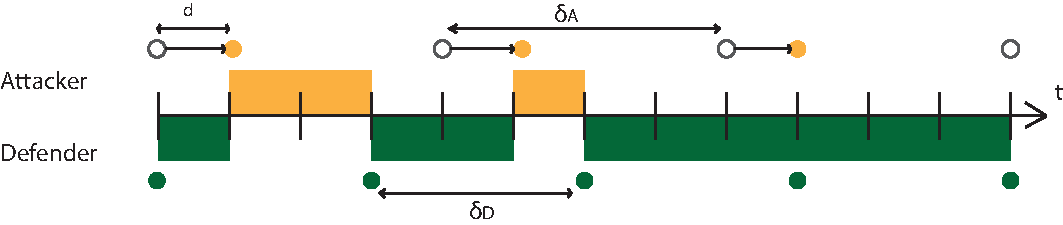
\includegraphics[scale=0.7]{Images/DefFlip.pdf}
\caption{Formalization of a FlipIt game with delay: A representation of a FlipIt game where both players are playing periodically. Every move or flip is indicated by a green or orange circle, respectively dark gray and light grey.  The defender is represented in green (dark grey) and plays with a period of $\delta_{D}$. The flip of the attacker is represented by a white circle, but because there is a delay d, the attacker only controls the resource after time d represented by an orange circle (light grey). The attacker plays with a period of $\delta_{A}$. The green and orange rectangles represent the amount of time the respective player is in control of the resource.}
\label{FlipItDelay}
\end{figure}

\begin{description}
\item $i$: Denotes the player. \textit{D} denotes the defender, and \textit{A} denotes the attacker which differs form the notation in \citep{FlipIt}, where the defender is denoted by the subscript \textit{0} and the attacker by the subscript \textit{1}.
\item $\delta_{i}$: The length of the interval between two consecutive moves of player \textit{i}. 
\item $\alpha_{i}$: The average flip rate of player \textit{i}, given by $\alpha_{i}=1/\delta_{i}$.
\item $k_{i}$: The cost of player \textit{i}'s moves.
\item $d$: The delay caused by the virus propagation.
\item $G_{i}(t)$: The total gain of player \textit{i}, which is the amount of time player \textit{i} is in control over the resource up to time \textit{t}.
\item $\gamma_{i}$: The average gain rate of player \textit{i}, defined as $G_{i}(t)/t$
\item $\beta_{i}$:  The average benefit rate up to time \textit{t}, defined as  $\beta_{i} = \gamma_{i} -k_{i} \alpha_{i} $.
\item $opt_{i}$: The optimum function for player \textit{i}. 
\end{description}

The adaptation of the FlipIt model starts from the assumption that, when an attacker attacks at time \textit{t}, he doesn't get immediate control over the resource, but he only gains control at time \textit{t + d}, with $d$ denoting the time needed to infect a sufficient number of (or all) nodes. If the defender flips the network before the period $d$ has elapsed (so, somewhere between $t$ and $t + d$), then the attacker will never gain full control over the resource. (See figure \ref{dt} at point 3 and 4). This implies that the mathematical formulas for gain and benefit need to be adapted to the fact that the attacker loses part of his benefit because of this delay. In the remainder of this paper, we will adapt the formalization of the FlipIt game using the delay variable $d$. \\ 

\begin{figure}[hbtp]
\centering
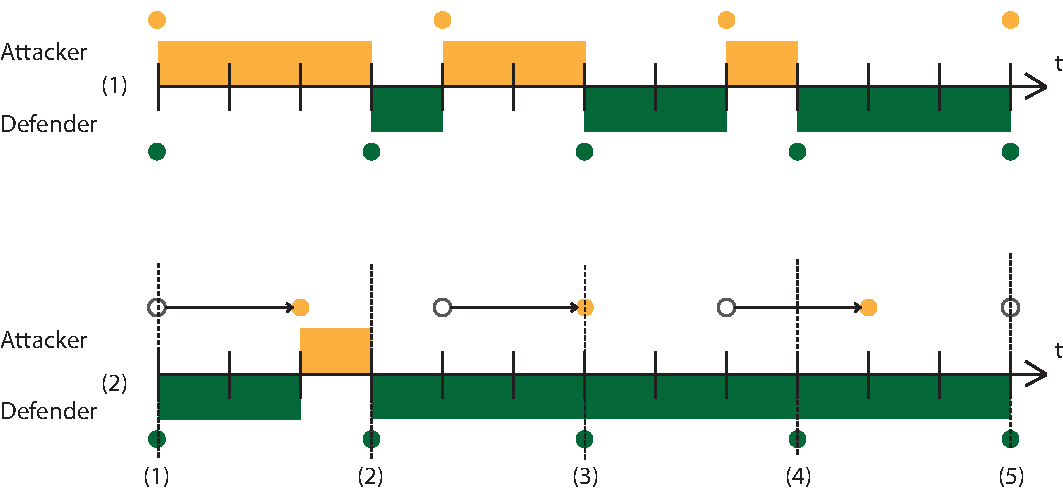
\includegraphics[scale=0.7]{Images/Delayuitgelegd.pdf}
\caption{The first game is the basic FlipIt game. The second is the FlipIt game with a delay. During the first flip of the attacker, the defender moves after the delay, causing the attacker to get control over the resource. During the second flip of the attacker, the defender flips at time t+d, causing the defender to take control over the resource before the attacker. During the third and final flip of the attacker, the defender flips during time t+d, causing the attacker to never gain control over the resource. }
\label{dt}
\end{figure}

Similarly as in \cite{FlipIt}, we split the formalization in two cases. In the first case the defender plays at least as fast as the attacker, in the second case the attacker plays at least as fast as the defender. For each of these cases, the benefit formula of the basic case without delay is presented first, and subsequently the delay is introduced.  \\

Intuitively, we could assume that $d$ can never be bigger than $\delta_{A}$ because then the attacker would play again before the delay has finished. This would seemingly result in a gain for the defender that is always 1, but this is not always true. Assume for example that an attacker plays with an interval of 3 time units, that the delay is equal to 4 time units and that the defender only plays every 8 time units. This situation is represented in figure \ref{langedelay}. Since the delay is shorter than the period of the defender, the attacker takes control of the resource once the delay has elapsed, until the defender plays. However, if the delay is larger that the period of the defender, then the defender will always be in control. This situation is represented in figure \ref{langeredelay}, where the attacker plays with an interval of 5 time units, the delay is equal to 6 time units and the defender plays with an interval of 4 time units. From this we can conclude that it only makes sense to calculate the formulas for the cases where $d$ is smaller than $\delta_{D}$. We can already conclude that it is of no use for the attacker to play when the delay is bigger than $\delta_{D}$. 




\begin{figure}[hbtp]
\centering
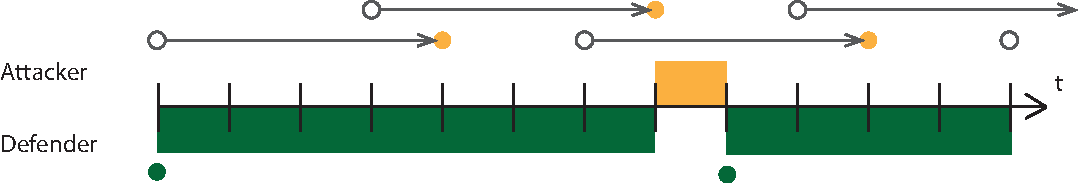
\includegraphics[scale=0.7]{Images/FlipItCase1delay.pdf} 
\caption{FlipIt with delay propagation where $\delta_{D} > d > \delta_{A}$.   }
\label{langedelay}
\end{figure}

\begin{figure}[hbtp]
\centering
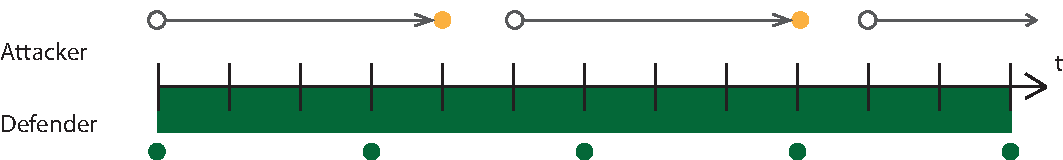
\includegraphics[scale=0.7]{Images/FlipItCase1delaytobig.pdf} 
\caption{FlipIt with delay propagation where $ d > \delta_{D}$ }
\label{langeredelay}
\end{figure}


In the original model of FlipIt \cite{FlipIt}, the authors express the formulas in terms of $\alpha_{D}$ and $\alpha_{A}$. However, when introducing the delay, some formulas become much simpler when expressed in terms of $\delta_{D}$ and $\delta_{A}$. Therefore in the remainder of this paper, we will formulate the model using both $\alpha_{i}$ and $\delta_{i}$, depending on which variable gives the simplest representation of the formulas.

\subsection*{\textbf{Case 1:} $\delta_{D} \leq \delta_{A} $ (The defender plays at least as fast as the attacker.) }

Let $r = \dfrac{\delta_{D}}{ \delta_{A} }$. The intervals between two consecutive defender's moves have length $\delta_{D}$. Consider a given defender move interval. The probability over the attacker's phase selection that the attacker moves in this interval is r. Given that the attacker moves within the interval, he moves exactly once within the interval (since $\delta_{D} \leq \delta_{A} $) and his move is distributed uniformly at random within this interval. \\

The expected period of attacker control within the interval as the moment on which the attacker gains control is uniformly distributed over the defender's interval. On average the attacker will gain control at time r/2. So the expected gain is equal to the remainder of the defender interval, i.e. r/2, without considering the delay by a virus. Therefore the benefit for the attacker, without considering the delay, can be expressed as follows:

\begin{equation*}
\beta_{A}(\delta_{D},\delta_{A}) =\dfrac {r} {2} - k_{A} \alpha_{A} = \dfrac {\delta_{D}} {2\delta_{A}} - k_{A} \alpha_{A}  
\end{equation*}\\

Correspondingly, the benefit for the defender can be expressed as:
\begin{equation*}
\beta_{D}(\delta_{D},\delta_{A}) =1 -  \dfrac {r} {2} - k_{D} \alpha_{D} = 1 - \dfrac {\delta_{D}} {2\delta_{A}} - k_{D} \alpha_{D} 
\end{equation*}

\begin{figure}[hbtp]
\centering
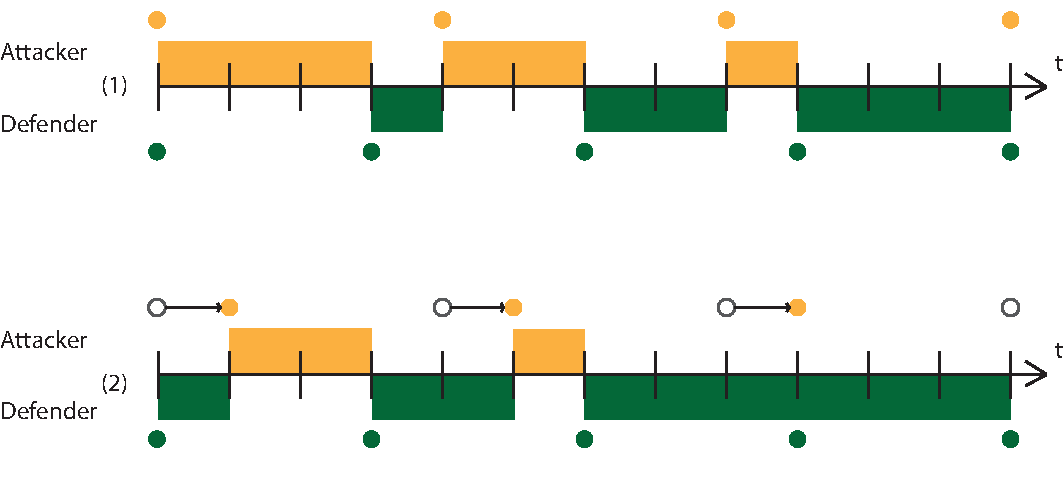
\includegraphics[scale=0.7]{../../doc/template/Images/DiffDelayCase1.pdf}
\caption{Case 1: Difference between a basic FlipIt game and a FlipIt game with a delay. Case (1) is the FlipIt game without a propagation delay and case (2) is with a propagation delay. The delay is denoted with an arrow. The attacker is only in control when the circle becomes orange (light grey).}
\label{fig:delaycase1}
\end{figure}




However, because of the delay required for virus propagation, the maximal time of control is reduced to $\delta_{D}-d$ , see figure \ref{fig:delaycase1}. While the probability that the attacker will move in the interval of the defender is still \textit{r}, the gain will not be half of the interval. Indeed, if the attacker plays after $\delta_{D}-d$, given the delay \textit{d}, he will never gain control in that interval (see figure \ref{tijdens interval}). 
\begin{figure}[hbtp]
\centering
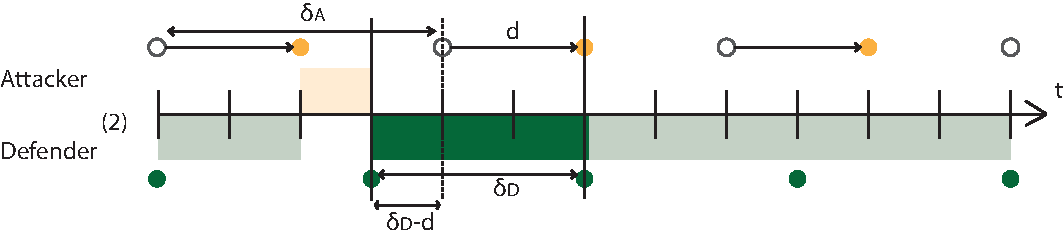
\includegraphics[scale=0.7]{../../doc/template/Images/delaydtijdens.pdf}
\caption{Attacker playing to late. If the attacker enters the defender's interval after $\delta_{D} -d$, he can not get in control in that interval.}
\label{tijdens interval}
\end{figure}The probability that the attacker plays early enough is $\dfrac{\delta_{D}-d}{\delta_{D}}$, giving the attacker an average gain of $\dfrac{\delta_{D}-d}{2}$ (the average remainder of the defender interval after the attacker flipped). If the attacker moves after the period of $\delta_{D}-d$, the gain of the attacker will be zero. The probability that this happens is  $\dfrac{d}{\delta_{D}}$. Looking at one interval of the defender, the average gain rate of the attacker can thus be expressed as follows:


\begin{equation*}
\gamma_{A}(\delta_{D},\delta_{A}) = \dfrac {1}{\delta_{D}} [ \dfrac{\delta_{D}}{\delta_{A}} \cdot \big[ \dfrac{\delta_{D}-d}{\delta_{D}} \cdot \dfrac{\delta_{D}-d}{2} + \dfrac{d}{\delta_{D}} \cdot 0 \big] ]
\end{equation*}
As the formula above is valid for each defender interval, the average gain rate over the entire game is:
\begin{equation*}
\gamma_{A}(\delta_{D},\delta_{A}) = \dfrac{(\delta_{D} -d)^{2}}{2\delta_{D}\delta_{A}}
\end{equation*}

To find the benefit, the cost of moving is subtracted from the average gain. 
\begin{equation}
\beta_{A}(\delta_{D},\delta_{A}) = \dfrac { (\delta_{D}-d) ^{2}} {2 \delta_{D}  \delta_{A}} - \dfrac{k_{A}}{\delta_{A}}
\label{Benfcase1:attacker}
\end{equation}

 
 The benefit of the defender is then as follows:
\begin{equation}
\beta_{D}(\delta_{D},\delta_{A}) = 1 - \dfrac { (\delta_{D}-d) ^{2}} {2 \cdot \delta_{D}  \delta_{A}} - \dfrac{k_{D}}{ \delta_{D}}
\label{Benfcase1:defender}
\end{equation}
~~\\
For this case where $d$=0, we this equals the formula of the original FlipIt game \citep{FlipIt} [p675].\\





\subsection*{\textbf{Case 2:} $\delta_{A} \leq \delta_{D} $ (The attacker plays at least as fast as the defender.) }

First let $r = \dfrac{\delta_{D}}{ \delta_{A} }$. The intervals between two consecutive attacker's moves have length $\delta_{A}$. Consider a given attackers move interval. The probability over the attacker's phase selection that the defender moves in this interval is $\dfrac{\delta_{A}}{ \delta_{D} } = (1/r)$. Given that the defender moves within the interval of the attacker, he moves exactly once within this interval (since $\delta_{A} \leq \delta_{D} $) and his move is distributed uniformly at random. \\

A similar analysis as in case 1 for a FlipIt game without a propagation delay yields the following benefits:

\begin{equation*}
\beta_{D}(\delta_{D},\delta_{A}) = \dfrac {1} {2r} - k_{D} \alpha_{D} = \dfrac {\delta_{A}} {2\delta_{D}} - \dfrac{k_{D} }{\delta_{D}} 
\end{equation*}
\begin{equation*}
\beta_{A}(\delta_{D},\delta_{A}) =1 - \dfrac {1} {2r} - k_{A} \alpha_{A} = 1- \dfrac {\delta_{A}} {2\delta_{D}} - \dfrac{k_{A}}{ \delta_{A}}  
\end{equation*}\\

An intuitive solution for the case with a virus would be to subtract the benefit of the attacker received in each interval with the delay similarly as in case 1. This would yield the following formula:
\begin{equation*}
\beta_{A}(\delta_{D},\delta_{A})=\dfrac{(\delta_{A} - d)^2}{2\delta_{A}\delta_{D}} - \dfrac{k_{D}}{\delta_{A}}
\end{equation*}

This however results in an overestimation. 
%By simulation the game, it can be notices that the closer $\delta_{A}/\delta_{D}$ is equal to one, the better the approximation. If $\delta_{A}/\delta_{D} = 1$ the result is correct. 
The reason this formula overestimates the benefit of the attacker is that it assumes that the defender is always in control during the delay. However, if the attacker was in control in the previous interval, then he continuous to be in control during the period of the delay, see figure \ref{fig:case2}. This means that the average benefit formulas for this case cannot be derived from one interval only; what happens in the previous interval must be taken into account. \\

We know that the defender's moves are instantaneous. Therefore, it is easier to calculate the benefit of the defender. Because the defender moves slower than the attacker we know that if the defender moves during the interval of the attacker, he only moves once within this interval.

The defender will move during the interval of the attacker with a probability of $\dfrac{\delta_{A}}{\delta_{D}} $. If this happens, the defender will be in control for the remainder of this interval. In the next interval the attacker will have to regain control, meaning that during the delay, the defender stays in control, see figure \ref{fig:case2} cases (1) to (4). The defender will keep the control over the resource in the next interval over a period of the delay, namely \textit{d}. \\

Consider a timespan $\delta_{A} + d$, representing the attacker's interval followed by the delay period in his next interval. If we assume that $\delta_{A}+d<\delta_{D}$, we can infer that the defender will never move twice during this timespan.
Because $d + \delta_{A} \leq \delta_{D}$ the next move of the defender in this second interval will never occur during the delay, meaning that the entire delay can be considered as an extra benefit resulting of a play in the previous interval. 
So, every time the defender plays, he will get an average gain of $\dfrac{\delta_{A}}{2}$ in the interval where he plays and in the next interval will always receive a extra gain of $d$, yielding a total average gain per interval of
$\dfrac{(d+\dfrac{\delta_{A}}{2})}{\delta_{A}}$

For the case with a delay we consider two cases, Case a and Case b, depending on whether the delay is shorter or longer than the difference between the attacker's and the defender's period.  \\

\begin{figure}[hbtp]
\centering
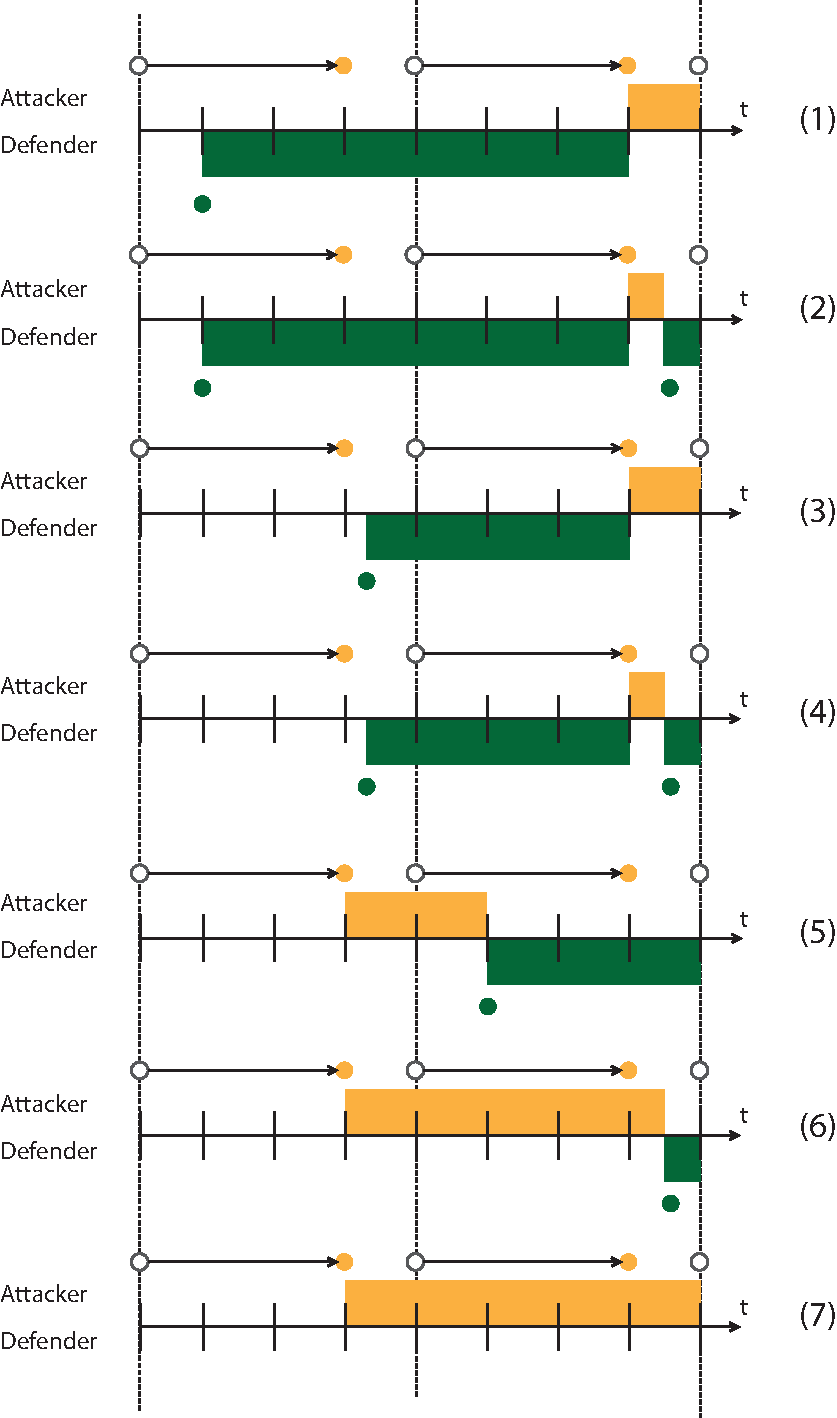
\includegraphics[scale=0.7]{../../doc/template/Images/FlipIt2.pdf}
\caption{All possible cases for the attacker and the defender in Case 2.A where $d + \delta_{A} < \delta_{D}$. As can be seen in cases (1) to (4), the defender will have control during a period of \textit{d} over the resource in the next interval when the defender has flipped in the previous interval.}
\label{fig:case2}
\end{figure}

\subsubsection*{\textbf{Case 2.a:} $ \delta_{D} \geq d + \delta_{A} \geq \delta_{A}$}
%The first case is where the defender's period is larger than the sum of the delay and the attacker's period. 
In this case the delay will never be counted twice in the defender's  benefit formula. To determine the total gain rate of the defender we need to know the probability that the defender will move during an interval and what the average time is that the defender controls the resource. Given that if the defender moves he will always benefit entirely from a period of delay in the next interval of the attacker, his total gain is $\dfrac{(d+\dfrac{\delta_{A}}{2})}{\delta_{A}}$ in one interval (as previously calculated. The total gain  rate of the defender is then the probability that the defender will move during an interval of the attacker multiplied by the total average gain per interval: 

\begin{equation*}\label{first}
\gamma_{D}(\delta_{D},\delta_{A}) = \dfrac{\delta_{A}}{\delta_{D}} \cdot \dfrac{(d+\dfrac{\delta_{A}}{2})}{\delta_{A}} 
\end{equation*}
\begin{equation*}\label{first}
\gamma_{D}(\delta_{D},\delta_{A}) = \dfrac{\delta_{A}}{2\delta_{D}} + \dfrac{d}{\delta_{D}} 
\end{equation*}\\
This yields the following benefit formula:
\begin{equation}\label{benfcase2a:defender}
\beta_{D}(\delta_{D},\delta_{A}) = \dfrac{\delta_{A}}{2\delta_{D}} + \dfrac{d}{\delta_{D}} - \dfrac{k_{D}}{ \delta_{D}}
\end{equation}\\

The benefit for the attacker will be as follows:
\begin{equation}\label{benfcase2a:attacker}
\beta_{A}(\delta_{D},\delta_{A}) = 1 -\dfrac{\delta_{A}}{2\delta_{D}} - \dfrac{d}{\delta_{D}} - \dfrac{k_{A}}{ \delta_{A}}
\end{equation}\\



It is crucial that $ \delta_{D}$ is at least as large as $d + \delta_{A}$. If not, the defender can move during the delay in the interval following the interval in which the defender already moved. This would result in an overlap between the average gain of $\dfrac{\delta_{A}}{2} +d$ and the delay. The above benefit formula would then include to much gain for the defender: the potential overlap during the delay would be counted twice. See figure \ref{countedtwice}\\

\begin{figure}[hbtp]
\centering
\caption{Cases where the delay would be counted twice.}
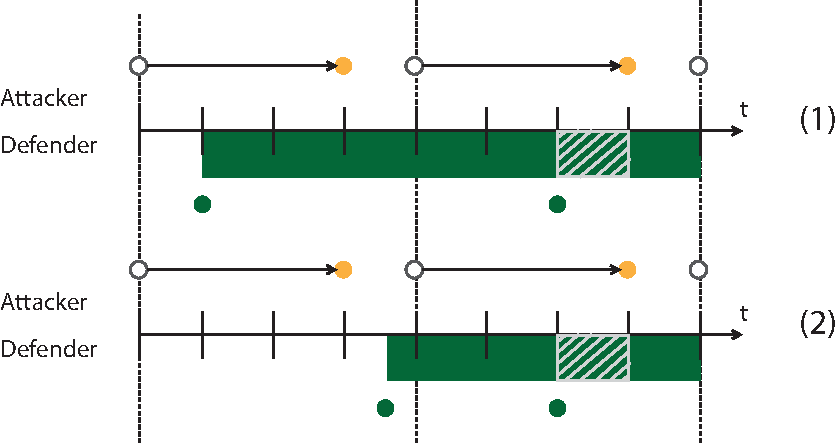
\includegraphics[scale=0.7]{Images/flipcase2nb.pdf}
\label{countedtwice}
\end{figure}

~~ \\
\subsubsection*{\textbf{Case 2.b:} $d + \delta_{A} \geq \delta_{D} \geq \delta_{A}$}
~~~\\

To obtain the formula in case of a too long delay, we therefore need to subtract this overlapping gain from the above formula. 
Since $\delta_{D} \geq \delta_{A}$, if the defender enters the interval immediately after the attacker has played, the defender cannot have played in the previous interval. In that case, there is no overlap. So the problem of the overlap only appears if the defenders enters late enough and thus only the last part of the delay is subject to overlap. The larger the difference between the interval of the defender and the attacker, the smaller the risk of overlap. Concretely, only the last part of length $d - (\delta_{D} - \delta_{A})$ is subject to overlap. Hence, the probability of overlap is $\dfrac{ d - (\delta_{D} - \delta_{A})}{\delta_{D}}$ and the average gain will be half of this interval:  $\dfrac{ d - (\delta_{D} - \delta_{A})}{2}$.  The gain rate to be subtracted is therefore:\\

\begin{equation*}
\dfrac{1} {\delta_{A}} \cdot \dfrac{d - (\delta_{D} - \delta_{A})}{\delta_{D}} \cdot \dfrac{d - (\delta_{D} - \delta_{A})}{2}
\end{equation*}

The total gain rate for the defender is obtained by subtracting this term from the gain rate of case a:
 \begin{equation*}
\gamma_{D}(\delta_{D},\delta_{A}) = \dfrac{\delta_{A}}{\delta_{D}} \cdot \dfrac{(d+\dfrac{\delta_{A}}{2})}{\delta_{A}} - \dfrac{(d - (\delta_{D} - \delta_{A}))^{2}}{2 \delta_{D} \delta_{A}}
\end{equation*}
\begin{equation*}
\gamma_{D}(\delta_{D},\delta_{A}) = \dfrac{\delta_{A}}{2\delta_{D}} + \dfrac{d}{\delta_{D}} - \dfrac{(d - (\delta_{D} - \delta_{A}))^{2}}{2 \delta_{D} \delta_{A}}
\end{equation*}\\
This yields in the following benefit formula:
\begin{equation}\label{benfcase2b:defender}
\beta_{D}(\delta_{D},\delta_{A}) = \dfrac{\delta_{A}}{2\delta_{D}} + \dfrac{d}{\delta_{D}} - \dfrac{k_{D}}{ \delta_{D}} - \dfrac{(d - (\delta_{D} - \delta_{A}))^{2}}{2 \delta_{D} \delta_{A}}
\end{equation}\\
 
Consequently, the benefit for the attacker will be:
\begin{equation}\label{benfcase2b:attacker}
\beta_{A}(\delta_{D},\delta_{A}) = 1 -\dfrac{\delta_{A}}{2\delta_{D}} - \dfrac{d}{\delta_{D}} - \dfrac{k_{A}}{ \delta_{A}} + \dfrac{(d - (\delta_{D} - \delta_{A}))^{2}}{2 \delta_{D} \delta_{A}}
\end{equation}\\

%~~\\
%\subsection{Conclusion of this chapter}
%\begin{description}
%\item[-]
%\item[-]
%\item[-]
%\end{description}



\chapter{Optimal Defence and Attack Strategies}
\label{chapter:Nash}
%\documentclass[10pt]{article}
%\begin{document}

%%%%%%%%%%%%%%%%%%%%%%%%%%%%%%%%%%%%%%%%%%%%%%%%%%%%%%%%%%
%%%%%			Introduction Chapter 1				%%%%%%
%%%%%												%%%%%%
%%%%%												%%%%%%
%%%%%%%%%%%%%%%%%%%%%%%%%%%%%%%%%%%%%%%%%%%%%%%%%%%%%%%%%%

%TODO-- rechtstreeks uit FlipIt paper --\\

In this chapter we are interested in finding the optimal defence and attack strategies. Ultimately, the optimal strategies can allow the determination of the Nash equilibria of the game. \\

%First the optimal functions are derived from the formulas in the previous chapter. From these piecewise functions we can derive the Nash equilibria. \\

Nash equilibria are points with the property that neither player benefits by deviating in isolation from the equilibrium. We can compute Nash equilibria for the periodic game as an intersection point of curves $opt_{D}$ and $opt_{A}$. 
\\
%As a second step, we are interested in finding Nash equilibria, points
%for which neither player will increase his benefit by changing his rate of play. 
More formally, a Nash equilibrium for the periodic game is a point $(\delta_{D}^{*},\delta_{A}^{*})$ such that
the defender's benefit $\beta_{D}(\delta_{D},\delta_{A}^{*}) $is maximised at $\delta_{D}= \delta_{D}^{*}$ and the attacker's benefit
$\beta_{A}(\delta_{D}^{*},\delta_{A}) $ is maximised at $\delta_{A}= \delta_{A}^{*}$.
To begin with, some useful notation. We denote by $opt_{D}(\delta_{A}$) the set of values (rates
of play $\delta_{D}$) that optimise the benefit of the defender for a fixed rate of play $\delta_{A}$ of the
attacker. Similarly, we denote by $opt_{D}(\delta_{D}$) the set of values (rates of play $\delta_{A}$) that optimise
the benefit of the attacker for a fixed rate of play $\delta_{D}$ of the defender. \\


% Fig \todo{fig} shows all the cases.\\
%\begin{figure}[hbtp]
%\centering
%\includegraphics[scale=0.4]{Images/bestresp.png}
%\caption{This figure shows the all the cases with their subcategories. 'A' stands for Case 2.A: $\delta_{D} \geq d+\delta_{A} \geq \delta_{A}$ and 'B' stands for Case 2.B: $d+\delta_{A} \geq \delta_{D} \geq  \delta_{A} $ }
%\label{grafiekbestr}
%\end{figure}

\section{Determining the Piecewise Functions $opt_{D}(\delta_{A})$}

To determine $opt_{D}(\delta_{A})$ we need to compute the derivative of  $\beta_{D}(\delta_{D},\delta_{A}) $ for a fixed $\delta_{A}$.
 We consider three cases for each piece of the piecewise function of $\beta_{D}$.
 
 
\subsection*{Case A: $\delta_{D} \leq d$}

The benefit formula obtained in the previous chapter is as follows:
\begin{equation}
\beta_{D}(\delta_{D},\delta_{A}) = 1 - \dfrac{k_{D}}{\delta_{D}}
\end{equation}


The function is of the type $1-1/x$, see figure \ref{1x}. The root of the benefit function  and the root of the first derivative are as follows:
\begin{equation}
\beta_{D}(\delta_{D},\delta_{A}) =0  ~~~~~~ =>~~~~~~\delta_{D} = k_{D} \\
\end{equation}
\begin{equation}
\dfrac{\partial \beta_{D}(\delta_{D},\delta_{A})}{\partial \delta_{D}} =0 ~~~~~~ =>~~~~~~ k_{D} = 0
\end{equation}

\begin{figure}[hbtp]
\centering
\includegraphics[scale=1]{Images/1x.png}
\caption{function of type $1-1/x$}
\label{1x}
\end{figure}

This means that if $\delta_{D} < k_{D}$  the function is negative and the defender will therefore not play, if $\delta_{D} > k_{D}$ the function is positive. If $k_{D} < 0$ the function will decrease and the defender will again not play (cost cannot be negative).  Assuming that costs are always non-negative $k_{D} > 0$, the function will increase, meaning that the slower the defender plays, the larger the benefit.



\subsection*{Case B: $ d \leq\delta_{D} \leq \delta_{A} + d$}
The defender's benefit formula obtained in the previous chapter in this case is as follows:
\begin{equation*}
\beta_{D}(\delta_{D},\delta_{A}) = 1 - \dfrac{\delta_{D}}{2\delta_{A}} - \dfrac{d^{2}}{2\delta_{D}\delta_{A}} + \dfrac{d}{\delta_{A}}  - \dfrac{k_{D}}{\delta_{D}}
\end{equation*}

To know if the function decreases or increases we take the partial derivative of this formula for a fixed $\delta_{A}$:
\begin{equation*}\label{formdelta}
\frac{\partial \beta_{D}(\delta_{D},\delta_{A})}{\partial \delta_{D}} = - \dfrac{1}{2\delta_{A}} + \dfrac{k_{D}}{\delta_{D}^{2}} + \dfrac{d^{2}}{2\delta_{D}^{2}\delta_{A}}
\end{equation*}
 
The stationary points (maximum, minimum) can be found by setting the first derivative equal to zero and finding the roots of the resulting equation:
\begin{equation*}
\frac{\partial \beta_{D}(\delta_{D},\delta_{A})}{\partial \delta_{D}} =0 ~~~~~~ =>~~~~~~ \delta_{D} = \sqrt{2\delta_{A}k_{D} + d^{2}}
\end{equation*}

Given the sign of the coefficient of $\delta_{D}^{2}$, this
leads to the following deduction: The function increases on $[0, \sqrt{2\delta_{A}k_{D} + d^{2}}]$ and is decreasing on $[\sqrt{2\delta_{A}k_{D} + d^{2}}, \infty]$. So we have a maximum at $\delta_{D} = min \{ \delta_{A} +d, \sqrt{2\delta_{A}k_{D} + d^{2}} \} $ and $\delta_{D}$ has to be larger than $d$. Taking the minimum of the two values is needed because $\delta_{D}$ cannot be larger than $\delta_{A} +d$. \\
~~\\


\subsection*{Case C: $\delta_{D} \geq d+\delta_{A} $ }

The benefit formula for the defender obtained in the previous chapter in this case is as follows:
\begin{equation*}
\beta_{D}(\delta_{D},\delta_{A})= \dfrac{\delta_{A}}{2\delta_{D}} + \dfrac{d}{\delta_{D}} - \dfrac{k_{D}}{\delta_{D}} = \dfrac{\delta_{A} + 2 (d-k_{D})}{2\delta_{D}}
\end{equation*}

Given that $\delta_{D}$ is always positive, the benefit function can be either increasing or decreasing depending on the numerator of the above fraction. \\

For $\delta_{A} + 2(d-k_{D}) > 0$ the benefit will be always positive but decreasing, see figure \ref{ShapeUp}. 
The defender will always play as fast as he can if $\delta_{A} + 2(d-k_{D}) > 0$ for $k_{D} < d$ or $k_{D} > d$ because $\delta_{A}$ will be positive in either case. There is an edge case if $d=k_{D}$, which results in a benefit of $\beta_{D}(\delta_{D},\delta_{A})= \dfrac{\delta_{A}}{2\delta_{D}}$. \\
\begin{figure}
\centering
\includegraphics[scale=0.5]{Images/ShapesUp.png} 
\caption{The benefit function is of the shape of 1/x and is always decreasing if $\delta_{A} + 2(d-k_{D}) > 0$. }
\label{ShapeUp}
\end{figure}

For $\delta_{A} + 2(d-k_{D}) < 0$, the benefit will always be increasing but negative so the defender will not play. See figure \ref{ShapeDown}.  \\

\begin{figure}
\centering
\includegraphics[scale=0.5]{Images/ShapeDown.png} 
\caption{The benefit function is of the shape of -1/x and is always increasing if $\delta_{A} + 2(d-k_{D}) < 0$.}
\label{ShapeDown}
\end{figure}
%The derivative of the above formula for a fixed $\delta_{A}$ results in the following:
%\begin{equation*}
%\frac{\partial \beta_{D}(\delta_{D},\delta_{A})}{\partial \delta_{D}} = -\dfrac{\delta_{A}}{2\delta_{D}^{2}} - \dfrac{d}{\delta_{D}^{2}} + \dfrac{k_{D}}{\delta_{D}^{2}}
%\end{equation*}
%The obtain the stationary points the first derivative is set equal to zero and the roots of the resulting equation are found:
%\begin{equation*}
%\frac{\partial \beta_{D}(\delta_{D},\delta_{A})}{\partial \delta_{D}} =0 ~~~~~~ =>~~~~~~ \delta_{A} = 2(k_{D}-d) = dk_{D} - 2d
%\end{equation*}
%
%This leads to the following deduction:
%\begin{description}
%\item If $k_{D} \leq d$ 
%\begin{description}
% \item $\beta_{D}$ will be decreasing but always positive. If we minimize $\delta_{D}$ the value of $\beta_{D}$ will be higher. 
%\end{description}
%\item If $k_{D} > d$ 
%\begin{description}
%\item if $ \delta_{A} > 2(k_{D} -d)$, \\
%$\beta_{D}$ will be decreasing but always positive. If we minimize $\delta_{D}$ the value of $\beta_{D}$ will be higher. 
%\item if  $\delta_{A} = 2(k_{D} -d)$, \\
%the benefit of the defender will be $\beta_{D}=0$.
%\item if $\delta_{A} < 2(k_{D} -d)$, \\
%$\beta_{D}$ will be increasing but always negative. In this case the defender will not play. 
%\end{description}
%\end{description}
~~\\

%\subsection*{Case 2.B: $d+\delta_{A} \geq \delta_{D} \geq  \delta_{A} $} 
%
%The benefit formula obtained in the previous chapter  (formula \ref{benfcase2b:defender}) for the defender in this case is as follows:
%\begin{equation*}
%\beta_{D}(\delta_{D},\delta_{A}) = \dfrac{\delta_{A}}{2\delta_{D}} + \dfrac{d}{\delta_{D}} - \dfrac{k_{D}}{\delta_{D}} - \dfrac{(d-(\delta_{D} - \delta_{A}))^{2}}{2\delta_{D}\delta_{A}}
%\end{equation*}
%
%The derivative of the above formula for a fixed $\delta_{A}$ results in the following:
%\begin{equation*}
%\beta_{D}(\delta_{D},\delta_{A}) =  - \dfrac{1}{2\delta_{A}} + \dfrac{k_{D}}{\delta_{D}^{2}} + \dfrac{d^{2}}{2\delta_{D}^{2}\delta_{A}}
%\end{equation*}
%
%
%The stationary points (maximum, minimum) can be found by setting the first derivative equal to zero and finding the roots of the resulting equation:
%
%\begin{equation*}
%\frac{\partial \beta_{D}(\delta_{D},\delta_{A})}{\partial \delta_{D}} =0 ~~~~~~ =>~~~~~~ \delta_{D} = \sqrt{2\delta_{A}k_{D} + d^{2}}
%\end{equation*}
%
%
%For case 2.B this leads to the following deduction, which results in the same formula as for case 1 but with a small difference for the value of $\delta_{D}$: The function increases on $[0, \sqrt{2\delta_{A}k_{D} + d^{2}}]$ and is decreasing on $[\sqrt{2\delta_{A}k_{D} + d^{2}}, \infty]$. Because $\delta_{D} \geq \delta_{A}$ there is a maximum on $\delta_{D} = maximum \{ \delta_{A}, \sqrt{2\delta_{A}k_{D} + d^{2}} \} $ or because $d+\delta_{A} \geq \delta_{D}$ there is also on $\delta_{D} = minimum \{ \delta_{A}+d, \sqrt{2\delta_{A}k_{D} + d^{2}} \} $. %-Remark- \todo{beter uitschrijven, deltaD moet tussen die twee waarden liggen}\\

\subsection{Best Responses of $\delta_{D}$}
The optimum functions will be piecewise functions. We distinguish six cases for different values of $\delta_{A}$ depending on the values of $k_{D}$ and $d$. 
%We point out that $\delta_{A}$ and $\delta_{D}$ are positive rates. 
Figure XXX shows on the left how the three cases can be combined in a single continuous function (shown as the thick line). On the right, the derivative function indicates at which points the benefit will change. It is interesting to note that the derivative is also continuous, meaning that the benefit function is smooth and has no rough edges or corners. This implies that there are no sudden changes in benefit for small changes of period.

\subsection*{$\delta_{A} < 2(k_{D} - d)$}
For case A, the function will always increase if $k_{D} > 0$. If $k_{D} < 0$ it means that the cost is negative and we assume a positive cost. The function will thus never decrease. $k_{D} =0$ is an edge case and will be covered later in the paragraph of edge cases. So for case A we can conclude that the function is always increasing. In the next case, case B, the benefit function will increase in the interval $[0, 2(k_{D}-d)[$. In case C, for $\delta_{A} < 2(k_{D} - d)$, the benefit function will always increase. Because for all the cases we are dealing with a negative benefit function that is increasing, the maximum benefit is achieved for $\delta_{} = \infty$. This can be seen in (A) in figure \ref{case1D}.

\begin{figure}[hbtp]
\centering
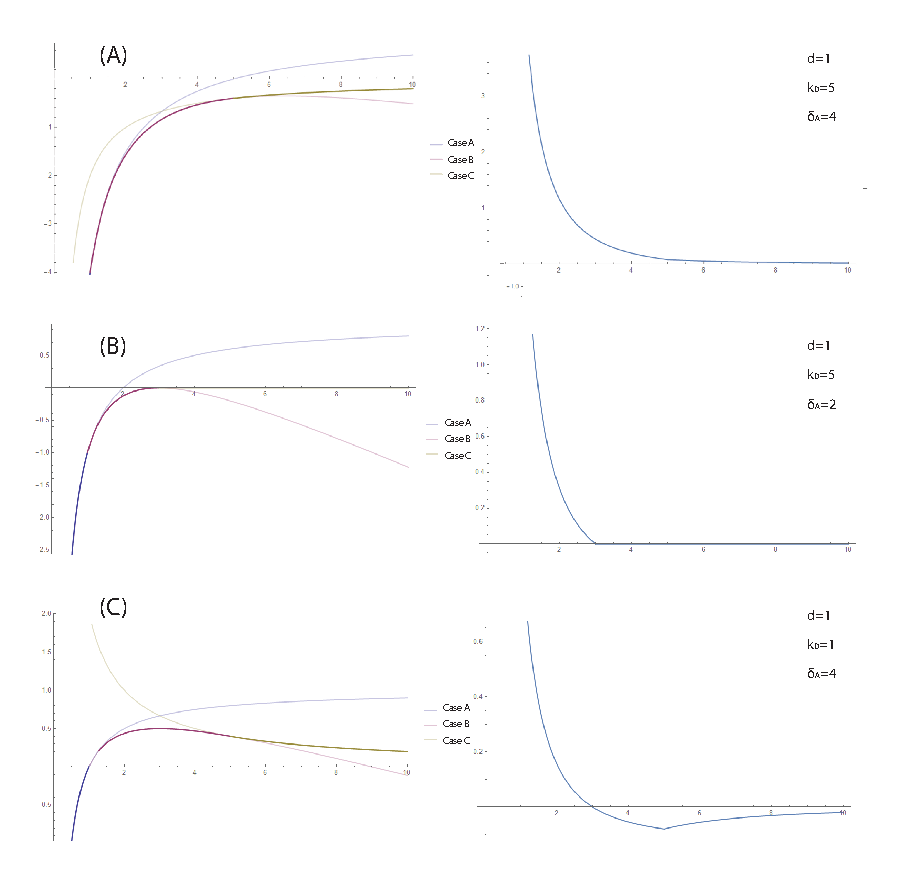
\includegraphics[scale=1]{Images/case1b.pdf}
\caption{ Illustration of the best response functions. The left functions are the piecewise benefit function of the defender for a certain values of $k_{D},d$ and $\delta_{A}$.. The right functions are the derivatives of the benefit functions on the left. The best responses are the values where the function intersects with the x-as. (A): $\delta_{A} < 2(k_{D}-d)$, (B): $\delta_{A} = 2(k_{D} - d)$, (C): $\delta_{A} > 2(k_{D} - d)$}
\label{case1D}
\end{figure}


%From case C above, it follows that if $\delta_{A} < 2(k_{D} - d)$ the benefit is increasing but it will always be non-positive. The defender will try not to play ($\delta_{D}= \infty$). 

%From case C it follows that from interval $[2(k_{D} -d), \sqrt{2k_{D}\delta_{A} + d^{2}}]$  (because for case 2 $\delta_{D} \geq \delta_{A}$), that the benefit is increasing.  The maximum of case 2.a and the maximum of case 2.b can be brought together. It follows that the optimal benefit is achieved at the $\delta_{D}=minimum[\delta_{A} + d, \sqrt{2k_{D}\delta_{A} + d^{2}}]$, which is $\delta_{D}=\sqrt{2k_{D}\delta_{A} + d^{2}}$. But because of case 2.a, the defender's maximum benefit is not to play at all.

\subsection*{$\delta_{A} = 2(k_{D} - d)$}
The delay can not be a negative value. So for $\delta_{A}$, a positive period, to be equal to  $2(k_{D} - d)$, $k_{D}$ has to be positive. \\
For case A, if $k_{D}>0$ the benefit function is always increasing. In case B, the value of $\delta_{A} =2(k_{D} - d)$ has to filled in in the root, $\sqrt{2k_{D}\delta_{A} + d^{2}}$. This gives the value $2k_{D}-d$. $2(k_{D}-d) < 2k_{D}-d$ so this means that $\delta_{A}$ is smaller than $ \sqrt{2k_{D}\delta_{A} + d^{2}}$, so the function is increasing. A maximum is achieved for $\delta_{D}$ equal to the maximum of $\left\lbrace \delta_{A}+d, \sqrt{2k_{D}\delta_{A} + d^{2}}\right\rbrace $. If we fill in $\delta_{A} = 2(k_{D} - d)$, the two values are the same so they are both a maximum.
If we fill in the value of $\delta_{A} = 2(k_{D} - d)$ in case C, the benefit will always be 0. Case C is the case for all values $\delta_{D} \geq \delta_{A} + d$, so $\beta_{D}=0$ is true for all $\delta_{D} \in [\delta_{A}+d, \infty]$.
The defender's maximum benefit is thus achieved for all $\delta_{D} \in [\sqrt{2k_{D}\delta_{A} + d^{2}}, \infty]$. See (B) in figure \ref{case1D}.

%For case C, $\beta_{D}(\delta_{D}, \delta_{A})=0$ for  all $\delta_{D} \in [\sqrt{2k_{D}\delta_{A} + d^{2}}, \infty]$. For case B, the benefit is increasing in the interval $[\delta_{A},\sqrt{2k_{D}\delta_{A} + d^{2}}]$. If we put both cases back together, we get a maximum at $\sqrt{2k_{D}\delta_{A} + d^{2}}$. So in this case the defender's maximum benefit is achieved for any $\delta_{D}$ in $[\sqrt{2k_{D}\delta_{A} + d^{2}}, \infty]$ with value 0.

\subsection*{$\delta_{A} > 2(k_{D} - d)$ }
Again for case A, we assume that $k_{D}$ is positive which implies that the benefit function for the defender is always increasing. If $\delta_{A} > 2(k_{D} - d)$, the benefit function of the defender in case B will only increase in the interval $]2(k_{D} - d), \sqrt{2k_{D}\delta_{A} + d^{2}}$. The maximum is achieved for $\delta_{D}$ equal to the maximum of $\left\lbrace \delta_{A}+d, \sqrt{2k_{D}\delta_{A} + d^{2}}\right\rbrace $. If we fill in $\delta_{A} > 2(k_{D} - d)$ , $\sqrt{2k_{D}\delta_{A} + d^{2}}$ is the maximum value. In case C, for all $\delta_{A} > 2(k_{D} - d)$, the benefit function is always decreasing. If we put all the pieces together, the defender's maximum benefit is achieved for $\delta_{D} = \sqrt{2k_{D}\delta_{A} + d^{2}}$. See (C) in figure \ref{case1D}.

%For case C, it follows that the benefit is decreasing but positive. So the defender will try to play as fast as possible ($\delta_{D} \rightarrow 0$). For case B it is increasing in the interval $[ 0,\sqrt{2k_{D}\delta_{A} + d^{2}}]$. It follows that the defender's maximum benefit is achieved for $\delta_{D} = \sqrt{2k_{D}\delta_{A} + d^{2}} $  \\


~~\\
From this analyses we can compute $opt_{D}(\delta_{A})$ : \\

 \begin{displaymath}
  opt_{D}(\delta_{A}) = \left\{
     \begin{array}{lr}
          \infty , & \delta_{A} < 2(k_{D} - d)\\
      \left[ \sqrt{2k_{D}\delta_{A} + d^{2}},\infty\right] , & \delta_{A} = 2(k_{D} - d) \\
      \sqrt{2k_{D}\delta_{A} + d^{2}}, & \delta_{A} > 2(k_{D} - d)
     \end{array}
   \right.
\end{displaymath}

~~\\


\subsection*{Edge cases:}

\subsection*{$\delta_{A}=0$ and $k_{D}=0$}

If $k_{D}=0$ it means that every flip of the defender is free. So for the cost it does not matter for the defender if he plays faster or slower. $\delta_{A}=0$ means that the attacker will play as fast as he can.  
\begin{itemize}
\item if $d=0$, if we look at $opt_{D}(\delta_{A})$ it means that we are in the second piece. The defender will play with a rate of $[0,\infty]$. 
\item if $d >0$, we have to look at the third piece of  $opt_{D}(\delta_{A})$ . Here it follows that the defender has to play with a rate of \textit{d}.
\end{itemize}

Combining those two leads to a rate for the defender equal to $[0,d]$. This means that the defender will never not play, which is intuitively correct if we know that the defender has no disadvantage to play because there is no cost involved.\\

Or more intuitively: If $\delta_{A}=0$ it means that the attacker is playing as fast as possible. For the defender it does not cost anything to flip, because $k_{D}=0$. We know that if $\delta_{D} \leq d$ the defender always has a benefit of 1. This means that for this case the defender will play with a rate $\delta_{D} \in [0,d]$.\\
\subsection*{$\delta_{A}=0$}
If $\delta_{A}=0$ it means that the attacker is playing as fast as possible. The defender has still a cost for every flip. This means we have to look at different values for $k_{D}$ and $d$.
\begin{itemize}
\item if $k_{D} > d$, it follows that the defender will not play (rate equal to $\infty$). This is already the case for the first piece in the piecewise function. $\delta_{A}$ will always be smaller than $2(k_{D}-d)$ if $k_{D} > d.$
\item if $k_{D}=d$, it corresponds to the second piece: the defender will play with a rate of $[d,\infty]$.
\item if $k_{D} < 0$, this corresponds with the last piece, where the rate of the defender is equal to \textit{d}.
\end{itemize}
By combining the last two pieces we have  $d ~~$for$~~ \delta_{A} =0 ~~$ and$ ~~k_{D} \leq d$.\\

\subsection*{$k_{D}=0$}
The cost of flipping for the defender is equal to zero. If we look at the benefit function of the defender and it's derivative in figure \ref{cost0}, we can see that the benefit for case B increases until $d$ and that the benefit in case A stays the same until $d$. After point $d$ the benefit decreases in all the cases. 

\begin{figure}[hbtp]
\centering
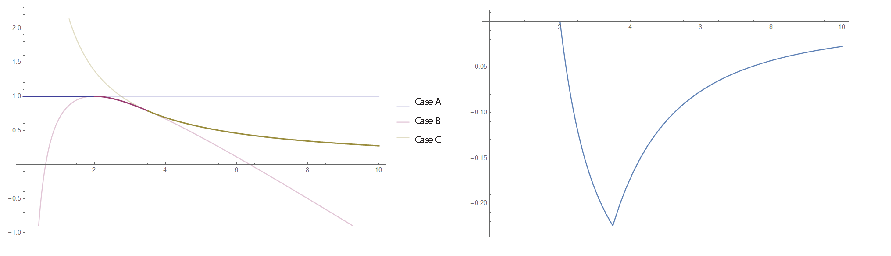
\includegraphics[scale=1]{Images/cost0.pdf} 
\caption{Benefit function and derivative for a cost $k_{D} = 0$ and with $d (=2)$ and $\delta_{A}=(1.5)$ not equal to zero.}
\label{cost0}
\end{figure}




\subsection{Conclusion}
Including the edge cases, $opt_{D}(\delta_{A})$ is as follows:  \\

 \begin{displaymath}
  opt_{D}(\delta_{A}) = \left\{
     \begin{array}{lr}
     \left[0,d\right] & \delta_{A} =0 ~~\& ~~k_{D}=0 \\
     \left[0,d\right] & k_{D}=0\\
     d & \delta_{A} =0 ~~ \& k_{D} \leq d\\
          \infty , & \delta_{A} < 2(k_{D} - d)\\
      \left[ \sqrt{2k_{D}\delta_{A} + d^{2}},\infty\right[ , & \delta_{A} = 2(k_{D} - d) \\
      \sqrt{2k_{D}\delta_{A} + d^{2}}, & \delta_{A} > 2(k_{D} - d)
     \end{array}
   \right.
\end{displaymath}
%*****************************************************************
%
% optimum functies voor beta A
%
%*********************************************************************
\section{Determining the Piecewise Functions $opt_{A}(\delta_{D})$}
%To start with we only consider the case where $d < \delta_{D}$, because if $d > \delta_{D}$ the benefit of the defender \todo{nakijken, def of att} is always 1. \\
To determine the optimal strategy of the attacker we also need to determine $opt_{A}(\delta_{D})$ by computing the derivative of $\beta_{A}(\delta_{D},\delta_{A})$ for a fixed $\delta_{D}$. We consider the three cases of the piecewise function of $\beta_{A}$: \\


\subsection*{Case A: $\delta_{D} \leq d$}

The benefit formula for the attacker for this case obtained in the previous chapter is as follows:
\begin{equation}
\beta_{A}(\delta_{D},\delta_{A}) =  - \dfrac{k_{A}}{\delta_{A}}
\end{equation}


The function is of the type $-1/x$, see figure \ref{1xx}. The root of the benefit function is as follows:
\begin{equation}
\beta_{A}(\delta_{D},\delta_{A}) =0  ~~~~~~ =>~~~~~~k_{D} = 0 \\
\end{equation}


\begin{figure}[hbtp]
\centering
\includegraphics[scale=1]{Images/1x.png}
\caption{function of type $-1/x$}
\label{1xx}
\end{figure}

This means that the optimal benefit is achieved for a value $\delta_{A}=0$.





\subsection*{Case B: $ \delta_{A} \leq \delta_{D} -d$ }
The benefit formula for the attacker for this case obtained from the previous chapter is as follows:
\begin{equation*}
\beta_{A}(\delta_{D},\delta_{A}) =1- \dfrac{\delta_{A}}{2\delta_{D}} - \dfrac{k_{A}}{\delta_{A}} - \dfrac{d}{\delta_{D}}
\end{equation*}
The derivative for a fixed $\delta_{D}$ is as follows:
\begin{equation*}
\dfrac{\partial \beta_{A}(\delta_{D},\delta_{A})}{\partial \delta_{A}} = \dfrac{-1}{2\delta_{D}} + \dfrac{k_{A}}{\delta_{A}^{2}}
\end{equation*}
The stationary points (maximum, minimum) can be found by setting the first derivative equal to zero and finding the roots of the resulting equation:
\begin{equation*}
\frac{\partial \beta_{A}(\delta_{D},\delta_{A})}{\partial \delta_{D}} =0 ~~~~~~ =>~~~~~~ \delta_{A} = \sqrt{2\delta_{D}k_{A}}
\end{equation*}
It follows that $\beta_{A}(\delta_{D},\cdot)$ is increasing on $[0,\sqrt{2k_{A}\delta_{D}}]$ and decreasing on $[\sqrt{2k_{A}\delta_{D}}, \infty]$ and thus has a maximum on $\delta_{A} = minimum \{\delta_{D} -d, \sqrt{2k_{A}\delta_{D}} \} $. The minimum between $\delta_{D}-d$ and $ \sqrt{2k_{A}\delta_{D}}$ is needed because $\delta_{A} $ cannot exceed $\delta_{D}-d$ in this case. \\

%\subsection*{Case 2.B: $d+\delta_{A} \geq \delta_{D} \geq  \delta_{A} $} 
%
%The benefit formula obtained from the previous chapter \ref{benfcase2b:attacker} for this case is as follows: 
%\begin{equation*}
%\beta_{A}(\delta_{D},\delta_{A}) = 1 - \delta_{A}}{2\delta_{D}} - \dfrac{d}{\delta_{A}} - \dfrac{k_{A}}{\delta_{A}} + \dfrac{(d-(\delta_{D}-\delta_{A})^{2}}{2\delta_{D}\delta_{A}} 
%\end{equation*}
%The derivative for a fixed $\delta_{D}$ is as follows:
%\begin{equation*}
%\dfrac{\partial \beta_{A}(\delta_{D},\delta_{A})}{\partial \delta_{A}} = -\dfrac{\delta_{D}}{2\delta_{A}^{2}} + \dfrac{k_{A}}{\delta_{A}^{2}} - \dfrac{d^{2}}{2\delta_{D}\delta_{A}^{2}} + \dfrac{d}{\delta_{A}^{2}}
%\end{equation*}
%The stationary points (maximum, minimum) can be found by setting the first derivative equal to zero and finding the roots of the resulting equation:
%\begin{equation*}
%\frac{\partial \beta_{A}(\delta_{D},\delta_{A})}{\partial \delta_{D}} =0 ~~~~~~ =>~~~~~~ \delta_{D}= \dfrac{(\delta_{D}-d)^{2}}{2k_{A}}
%\end{equation*}
%
%
%It follows that $\beta_{A}(\delta_{D},\cdot)$ is increasing and non-positif if $\delta_{D} > \dfrac{(\delta_{D}-d)^{2}}{2k_{A}}$ and decreasing and positive if $\delta_{D} < \dfrac{(\delta_{D}-d)^{2}}{2k_{A}}$. This is the same result as in case 1.\\

\subsection*{Case C: $d \leq \delta_{D} -d \leq \delta_{A} $}

The benefit formula for the attacker for this case obtained in the previous chapter is as follows:
\begin{equation*}
\beta_{A}(\delta_{D},\delta_{A}) =\dfrac{\delta_{D}}{2\delta_{A}} - \dfrac{k_{A}}{\delta_{A}} + \dfrac{d^{2}}{2\delta_{D}\delta_{A}} - \dfrac{d}{\delta_{A}}
\end{equation*}
The derivative for a fixed $\delta_{D}$ is as follows:
\begin{equation*}
\dfrac{\partial \beta_{A}(\delta_{D},\delta_{A})}{\partial \delta_{A}} = -\dfrac{\delta_{D}}{2\delta_{A}^{2}} + \dfrac{k_{A}}{\delta_{A}^{2}} - \dfrac{d^{2}}{2\delta_{D}\delta_{A}^{2}} + \dfrac{d}{\delta_{A}^{2}} = \dfrac{-\delta_{D}^{2} - d^{2} + 2\delta_{D}d + 2\delta_{D}k_{A}}{2\delta_{A}^{2}\delta_{D}}
\end{equation*}
The stationary points (maximum, minimum) can be found by setting the first derivative equal to zero and finding the roots of the resulting equation:
\begin{equation*}
\frac{\partial \beta_{A}(\delta_{D},\delta_{A})}{\partial \delta_{D}} =0 ~~~~~~ =>~~~~~~  \delta_{D}^{2}-\delta_{D}(2k_{A}-2d) + d^{2}= 0
\end{equation*}

The roots of this quadratic equation are $\delta_{D}=d+k_{A}\pm \sqrt{2dk_{A}+k_{A}^{2}}$. Because for this case $d\leq \delta_{D}$, we only look at root $\delta_{D}=d+k_{A} + \sqrt{2dk_{A}+k_{A}^{2}}$. $\sqrt{2dk_{A}+k_{A}^{2}}$ is bigger than $k_{A}$ so if we subtract it from $d+k_{A}$, we are in the part where $delta_{D}$ is smaller than d. \\
It follows that $\beta_{A}(\delta_{D},\delta_{A})$ is increasing and non-positive if $\delta_{D}> d+k_{A} + \sqrt{2dk_{A}+k_{A}^{2}}$ and decreasing and positive if $\delta_{D} < d+k_{A} + \sqrt{2dk_{A}+k_{A}^{2}}$. \\

\subsection{Best Responses of $\delta_{A}$}
The optimum function of the attacker is found in the same way as the optimum function of the defender. The derivatives of each piece of the piecewise benefit function of the attacker is taken. From these derivatives the best responses are derived. \\
Case A is an edge case and will be addressed in the paragraph about the edge cases.
%The optimum functions will be piecewise functions. We distinguish three cases for different values of $\delta_{D}$ regarding $d$ and $k_{A}$. 
%
%
%For this term $\dfrac{(\delta_{D}-d)^{2}}{2k_{A}} $ , $d$ has to be bigger than  $\delta_{D}$ because the cost $\delta_{D}$ cannot be negative. This was an assumption that was already made, because the benefit of the defender will always be 1 if $d$ is bigger than  $\delta_{D}$.

\subsubsection*{$\delta_{D} < d+k_{A} + \sqrt{2dk_{A}+k_{A}^{2}}$} 
For case B, the function is increasing. The function has a maximum on on $\delta_{A} = minimum \{\delta_{D} -d, \sqrt{2k_{A}\delta_{D}} \} $. For $\delta_{D} < d+k_{A} + \sqrt{2dk_{A}+k_{A}^{2}}$, the minimum of the two values is $\delta_{D}-d$.\\
For case C, if $\delta_{D} < d+k_{A} + \sqrt{2dk_{A}+k_{A}^{2}}$, the benefit function is increasing. Because we have a continuous function and the benefit is still increasing and negative in case C, the defender will try not to play. The defender's optimum benefit is achieved in $\delta_{A}=\infty$. See (A) in figure \ref{case1A}.

\begin{figure}[hbtp]
\centering
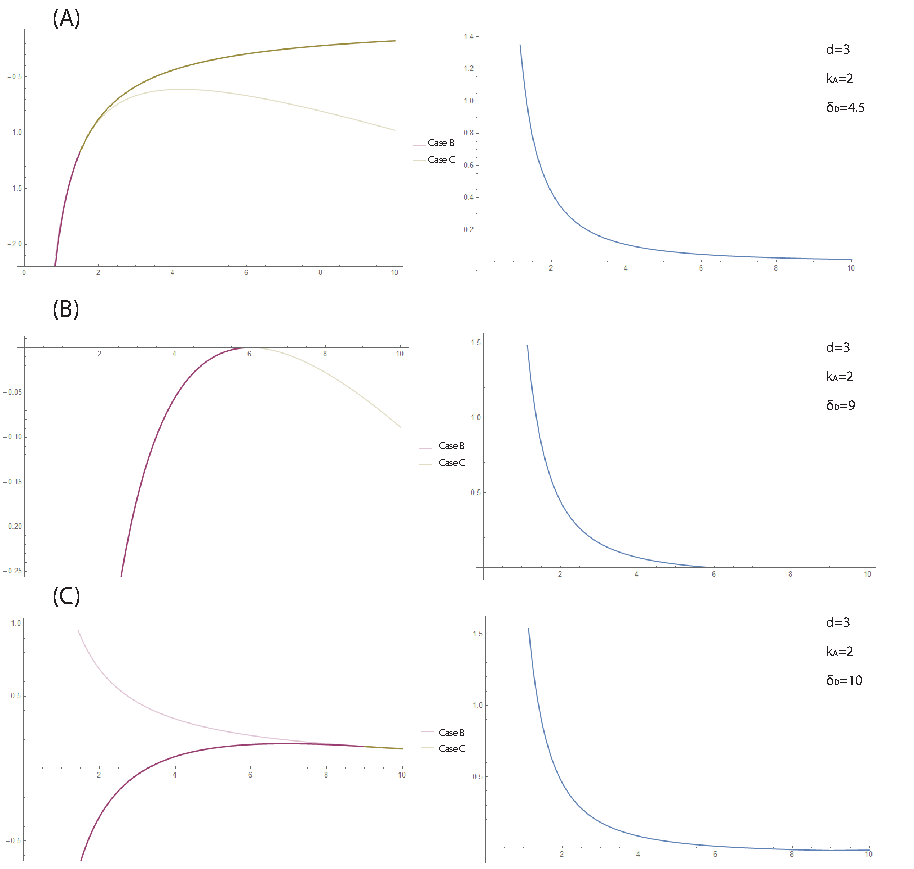
\includegraphics[scale=1]{Images/case1A.pdf}
\caption{ Illustration of the best response functions. The left functions are the piecewise benefit function of the attacker for a certain values of $k_{A},d$ and $\delta_{D}$. The right functions are the derivatives of the benefit functions on the left. The best responses are the values where the function intersects with the x-as. (A): $\delta_{D} > d+k_{A} + \sqrt{2dk_{A}+k_{A}^{2}}$, (B): $\delta_{D} = d+k_{A} + \sqrt{2dk_{A}+k_{A}^{2}}$, (C): $\delta_{D} < d+k_{A} + \sqrt{2dk_{A}+k_{A}^{2}}$}.
\label{case1A}
\end{figure}

%From case 1 and case 2.b above, it follows that the benefit is decreasing but positive, which means that the attacker will play as fast as he can. For case 2.a  $\delta_{D} \geq \delta_{A}$ is increasing. It follows that for this case the attacker's maximum benefit is achieved for $\delta_{A} = \sqrt{d k_{A}\delta_{D}}$.
%. In this case the attacker's maximum benefit is reached at $\delta_{A} = \delta_{A} = \sqrt{dk_{A}\delta_{D}}$  .
\subsubsection*{$\delta_{D} = d+k_{A} + \sqrt{2dk_{A}+k_{A}^{2}}$} 
For case B, the function is increasing. The function has a maximum on on $\delta_{A} = minimum \{\delta_{D} -d, \sqrt{2k_{A}\delta_{D}} \} $. For $\delta_{D} = d+k_{A} + \sqrt{2dk_{A}+k_{A}^{2}}$, the minimum of the two values is $\delta_{D}-d$.\\
For case C, $\delta_{D} = d+k_{A} + \sqrt{2dk_{A}+k_{A}^{2}}$ is a root so the benefit function of the attacker will be equal to zero. Because case C is the case where $\delta_{A}$ has to be bigger or equal to $\delta_{D}-d$, $\beta_{A}=0$ is valid for all $\delta_{A} \in [\delta_{D}-d,\infty]$.\\
Putting the pieces together gives us the optimum benefit for the attacker for all $\delta_{A} \in [\delta_{D}-d,\infty]$. See (B) in figure \ref{case1A}.

%The benefit $\beta_{A}(\delta_{D},\delta_{A})=0$ for case 1 and case 2.b for all $\delta_{D}$ in $[0, \infty [$. For case 2.a it follows that the benefit is increasing. The attacker's maximum benefit is achieved at any $\delta_{A} $ in 
\subsubsection*{$\delta_{D} > d+k_{A} + \sqrt{2dk_{A}+k_{A}^{2}}$} 
For case B, the function is increasing. The function has a maximum on on $\delta_{A} = minimum \{\delta_{D} -d, \sqrt{2k_{A}\delta_{D}} \} $. For $\delta_{D} > d+k_{A} + \sqrt{2dk_{A}+k_{A}^{2}}$, the minimum of the two values is $\delta_{D}-d$.\\
For case C, if $\delta_{D} > d+k_{A} + \sqrt{2dk_{A}+k_{A}^{2}}$ the function is decreasing. So the optimum benefit for all the cases is when $\delta_{D} = \delta_{D}-d$. See (C) in figure \ref{case1A}.\\
%For case 1 and case 2.b the benefit is increasing but non-positive. This means that the attacker won't play ($\delta_{A} = \infty$). 


From this analyses we can compute $opt_{A}(\delta_{D})$ : 

 \begin{displaymath}
  opt_{A}(\delta_{D}) = \left\{
     \begin{array}{lr}
            \infty & \delta_{D} < d+k_{A} + \sqrt{2dk_{A}+k_{A}^{2}} \\
       \left[ \delta_{D}-d, \infty\right],  & \delta_{D} = d+k_{A} + \sqrt{2dk_{A}+k_{A}^{2}} \\
    	\delta_{D}-d, & \delta_{D} > d+k_{A} + \sqrt{2dk_{A}+k_{A}^{2}}
     \end{array}
   \right.
\end{displaymath}
\\

\subsection*{Edge cases:}

\subsection*{$\delta_{D}=0$ and $k_{A}=0$}
If $\delta_{D}=0$, looking at the benefit formula of the attacker, it follows that the period of the defender will always be equal or smaller than the delay. The delay cannot be negative. So from case $\delta_{D} \leq d$ it follows that the attacker will always have a benefit equal to zero, because $k_{A}=0$. For the attacker it does not matter what he plays. The benefit will always be the same. The optimal strategy in this case for the attacker will be playing at a rate $\delta_{A} \in [0,\infty ]$.

\subsection*{$k_{A}=0$}
If the cost of playing for the attacker is zero, the attacker can play as fast as he can.  If $\delta_{D} \leq d$, looking at the benefit formula for the attacker, it does not matter what the attacker does, his benefit will always be zero. He will play with a rate $\delta_{A} \in [0,\infty ]$.  We can merge this with the previous case where $\delta_{D}=0$ and $k_{A}=0$.  If $\delta_{D} > d$, the attacker will play. He will play with a rate of $\delta_{A} \in [0, \delta_{D} - d ]$. 
\subsection*{$\delta_{D}=0$}
If $\delta_{D}=0$ it follows from the case $\delta_{D} \leq d$ that the attacker will always have a negative benefit, unless the cost is zero. If the cost is zero we have again the case of $\delta_{D}=0$ and $k_{A}=0$. But if the cost is non-zero, the optimal strategy of the defender is not moving at all. 

\subsection{Conclusion}
Including the edge cases yields the following for $opt_{A}(\delta_{D})$ : \\

 \begin{displaymath}
  opt_{A}(\delta_{D}) = \left\{
     \begin{array}{lr}
     \infty & \delta_{D} = 0 \\
     \left[0,\infty\right] & \delta_{D} \leq d ~~\& ~~k_{A}=0 \\
          \left[0,\delta_{D} - d\right] & \delta_{D} > d ~~\& ~~k_{A}=0 \\
            \infty & \delta_{D} < d+k_{A} + \sqrt{2dk_{A}+k_{A}^{2}} \\
       \left[ \delta_{D}-d, \infty\right],  & \delta_{D} = d+k_{A} + \sqrt{2dk_{A}+k_{A}^{2}} \\
    	\delta_{D}-d, & \delta_{D} > d+k_{A} + \sqrt{2dk_{A}+k_{A}^{2}}
     \end{array}
   \right.
\end{displaymath}
\\

\section{Conclusion}

The piecewise functions $opt_{D}$ and $opt_{A}$ give some interesting results. 

\begin{itemize}
\item When the defender plays faster than the delay, the attacker will either have a negative benefit or a benefit equal to zero if the flips do not cost anything. It is for the defender a target to be able to play at a rate smaller or equal to the delay.
\item If the defender can play with a cost equal to zero, the attacker will not play. The defender can play at any rate he wants, and the attacker is always disadvantaged by his delay.
\item If the cost of the defender is non-zero, then, depending on the ratio between it's cost and the delay, from a certain value for the speed of the attacker, the defender will not play. The same thing goes for the attacker. This result is similar to the results obtained for the original FlipIt game.
\end{itemize}

The Nash Equilibria can be found as the intersection points of the piecewise functions $opt_{A}(\delta_{D})$ and $opt_{D}(\delta_{A})$. For this we have to compare the function in terms of the relationship of the players move cost. %We distinguish three cases: $k_{A} < k_{D} , ~k_{A} > k_{D} $ and $k_{A} = k_{D}$. 

\chapter{Virus Propagation }
\label{chapter4: Virus propagation}

\section{Methods of virus propagation}

The spreading of worms has already been extensivly researched [beter schrijven]. Because of all the different types of propagation it is hard to pick out one model that can model all of them. Modelling the spread of malware depends on two great factors: the method used for the propagation and the graph where the malware will spread itself. Viruses and worms are the types of malware that are the most researched. Under we list a couple of examples to model virus and worm propagation. In this text worm and virus will be used intermediate. 

\subsection{Models of graph representing the network}

\subsection*{Methods of propagation}

\begin{description}
\item Random scanning: Some worms propagate by using the method of random scanning 
IP addresses.  Rate of terms of succeeded randwomly choosen IP adresses -> maximise good ip adresses. After a while the remaining nodes will be les likely to be reached. An example of such a worm is `Code Red' .
\item Routing worms: they use BGP routing tables to scan the routable address space. 3 times faster than traditional worm that uses random scanning. Spyb0t or network bluepill.
\item email worms: use the email systems to propagate. The Kak worm is a Javascript computer worm that spread itself by exploiting a bug in Outlook Express. 
%Pikachu worm: The virus was mainly spread through Microsoft Outlook email attachments. The email containing the attached virus propagated through infected users by sending itself to all contacts in the user's Outlook address book. [5]
\item self stopping worm: reduces speed to avoid detection. Atak worm or self stopping worm
\end{description}

The start of such a propagation can be different. Either it is a targeted attack or a random attack. For example a usb stick or other shared resources can be used to start the spreading. It can be given to some special person or it can just be left behind in a parking lot. This can still be a targeted attack if it is the parking lot of a targeted company but there is more insecurity of where the usb stick will end. Another way is by sending an email. It can also start from one computer that is connected directly to the internet. Downloading malicious programs. 

\subsection*{Models for worm propagation}
To use the models for worm propagation in our model of the FlipIt game it is suffi"ent to know the propagation speed of the worm and define after how many time units the network is defected. This will be equal to the \textit{d} parameter in our model.  
Stackelberg game: first move is from attacker, defender is follower. 

Kind of network model: 
Kind of model: SIS, SIR

\subsubsection*{SIS}

\subsubsection*{SIR}

\subsubsection*{self disciplinary worms}
Model for self disciplinary worms and counter measures ... []

Popular mechanism that worms use to detect vulnerable targets by random ip scanning probing. Feasible due to use 32-bit addresses. 128-bit adresses life harder for worms, except the ones that use email systems to propagate. two new strategies: uniformly distributed random number generator to select new target. :spread locally, by biasing the search space towards addresses within the same subnet or network. 
The second strategy is almost the same as what email virusses would get. For this reason we work an example out .. 



A method to calculate the propagation of the virus in an easy way. Google page ranking algorithm. 



\section{methode met matrixen}

%$N_{0}$ denotes the initially infected resources at the beginning of the virus propagation. 
%$P_{x}(R_{n},t|R_{0},r,t_{0})$ denotes the chance that resource $R_{n}$ is infected at time $t$ after dropping virus number x on to resource $R_{0}$ at $t_{0}$ with rate $r$. \\

%$S(R_{n},R_{0})$ denotes the shortest path from the infected resource $R_{0}$ to resource $R_{n}$. It gives back a value with the distance measured with how many resources are in between including the end resource. \\

%So the chance that a resource is infected after time t is the chance that the resource is infected by all the previous infections and that the defender has not flipped the resource.
source: \url{http://en.wikipedia.org/wiki/Adjacency_matrix} \\
We model the network through an undirected Graph $G = < V, E> $ where $|V|$ denotes the number of resources in the network and $|E|$ the number of connections. We can convert this to a adjacent matrix where we can represent which vertices of the graph are neighbours of other vertices. \\
For our graph we have an $|V| \times |V|$ matrix with on every entry $a_{ij}$ a 1 as value if there is a connection between node $V_{i}$ and $V_{j}$ and with zeros its diagonal. Because our graph is undirected we have a symmetric matrix. 

\textit{"If \textit{A} is the adjacency matrix of the directed or undirected graph \textit{G}, then the matrix $A^{n}$ (i.e., the matrix product of n copies of \textit{A}) has an interesting interpretation: the entry in row i and column j gives the number of (directed or undirected) walks of length n from vertex i to vertex j. If n is the smallest nonnegative integer, such that for all i ,j , the (i,j)-entry of $A^{n} > 0$, then n is the distance between vertex i and vertex j."} [Wikipedia]

%%% Local Variables: 
%%% mode: latex
%%% TeX-master: "thesis"
%%% End: 
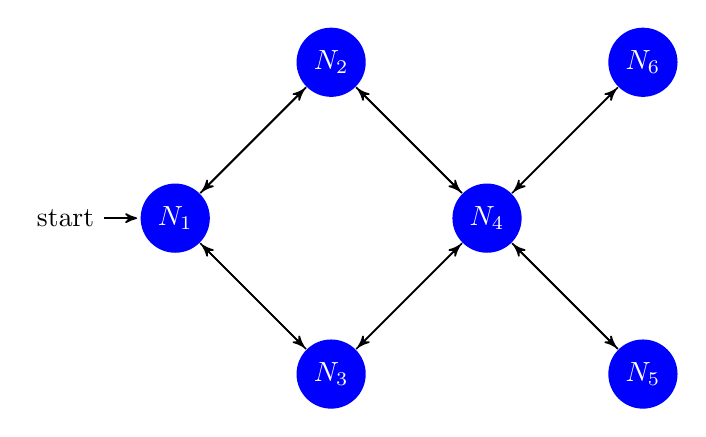
\begin{tikzpicture}[->,>=stealth',shorten >=1pt,auto,node distance=2.8cm,
                    semithick]
  \tikzstyle{every state}=[fill=blue,draw=none,text=white]

  \node[initial,state] (A)                    {$N_1$};
  \node[state]         (B) [above right of=A] {$N_2$};
  \node[state]         (D) [below right of=A] {$N_3$};
  \node[state]         (C) [below right of=B] {$N_4$};
  \node[state]         (E) [below right of=C] {$N_5$};
  \node[state]		   (F) [above right of=C] {$N_6$};

  \path (A) edge              node {} (B)
            edge              node {} (D)
        (B) edge              node {} (A)
        	edge			  node {} (C)
        (C) edge              node {} (B)
            edge 			  node {} (D)
            edge			  node {} (E)
            edge			  node {} (F)
        (D) edge 			  node {} (C)
            edge              node {} (A)
        (E) edge 			  node {} (C)
    	(F)	edge			  node {} (C);
\end{tikzpicture}
\\
%\[
%\begin{bmatrix}
%    x_{11}       & x_{12} & x_{13} & \dots & x_{1n} \\
%    x_{21}       & x_{22} & x_{23} & \dots & x_{2n} \\
%    \hdotsfor{5} \\
%    x_{d1}       & x_{d2} & x_{d3} & \dots & x_{dn}
%\end{bmatrix}
%=
%\begin{bmatrix}
%    x_{11} & x_{12} & x_{13} & \dots  & x_{1n} \\
%    x_{21} & x_{22} & x_{23} & \dots  & x_{2n} \\
%    \vdots & \vdots & \vdots & \ddots & \vdots \\
%    x_{d1} & x_{d2} & x_{d3} & \dots  & x_{dn}
%\end{bmatrix}
%\] 
The adjacent matrix becomes this matrix $[A]$: \\


$
\bordermatrix{
         & N_1		& N_2	& N_3	& N_4 	& N_5	&N_6     \cr
    N_1   & 0		& 1		& 1		& 0		& 0		& 0	     \cr
    N_2   & 1		& 0		& 0		& 1		& 0		& 0	     \cr
    N_3   & 1		& 0		& 0		& 1		& 0		& 0	     \cr
    N_4   & 0		& 1		& 1		& 0		& 1		& 1	     \cr
	N_5   & 0		& 0		& 0		& 1		& 0		& 0	     \cr
	N_6   & 0		& 0		& 0		& 1		& 0		& 0	     \cr
}$
\\

Matrix $A \times A = A^{2}$ becomes the matrix with the number of paths with 2 steps from $N_{i}$ to $N_{j}$: We denote this matrix as matrix \textit{[B]}\\


$
\bordermatrix{
         & N_1		& N_2	& N_3	& N_4 	& N_5	&N_6     \cr
    N_1   & 2		& 0		& 0		& 2		& 0		& 0	     \cr
    N_2   & 0		& 2		& 2		& 0		& 1		& 1	     \cr
    N_3   & 0		& 2		& 2		& 0		& 1		& 1	     \cr
    N_4   & 2		& 0		& 0		& 4		& 0		& 0	     \cr
	N_5   & 0		& 1		& 1		& 0		& 1		& 1	     \cr
	N_6   & 0		& 1		& 1		& 0		& 1		& 1	     \cr
}$
\\

Matrix $A^{2} \times A = A^{3}$ becomes the matrix with the number of paths with 3 steps from $N_{i}$ to $N_{j}$: We denote this matrix as matrix \textit{[C]}\\


$
\bordermatrix{
         & N_1		& N_2	& N_3	& N_4 	& N_5	&N_6     \cr
    N_1   & 0		& 4		& 4		& 0		& 2		& 2	     \cr
    N_2   & 4		& 0		& 0		& 6		& 0		& 0	     \cr
    N_3   & 4		& 0		& 0		& 6		& 0		& 0	     \cr
    N_4   & 0		& 6		& 6		& 0		& 4		& 4	     \cr
	N_5   & 2		& 0		& 0		& 4		& 0		& 0	     \cr
	N_6   & 2		& 0		& 0		& 4		& 0		& 0	     \cr
}$ 
\\

So for $A^{N}$ every $a_{ij}$ entry gives the number of paths with N steps from $N_{i}$ to $N_{j}$.\\

With this knowledge we can calculate in how many steps a node is infected. $A$ calculates which nodes are infected after 1 step, $A^{N}$ calculates which nodes are infected in N steps.. So if we want to know how many nodes are infected after 3 steps we have to add every matrix $(A + A^{2} + A^{3}) $ and see which entry is a non zero entry. 

What do we need for an algorithm
\begin{description}
\item Graph network $G = < V, E>$
\item Graph matrix $[A]$ which is $|V| \times |V| $
\item Attack vector $[X]$ which is $1 \times |V|$
\item cummulative matrix $[M]$ which is $|V| \times |V|$
\item state matrix $[T]$  which is $|V| \times |V|$
\item Reset vector $[R]$
\item duration \textit{d}
\item time \textit{n}
\item rate $\delta _{0}$ of defender and $\delta _{1}$ of attacker
\end{description}



Initialisation algorithm:


\begin{verbatim}
initialisatie
	d=0
	A=basismatrix
	M=A^{0}
	n=0
	\delta_{0}
	\delta_{1}
	X
	R
	controller = defender
	
	

	Algorithm
	n:= n + 1;
	Check who is in control? ( through modulo )
	if ( defender & controller=defender)
				d:= d + 1;
	
	if ( defender & controller=attacker )
				G = X \times R  (flippen ten voordele van defender)
				d = 0
				controller = defender
				
	if ( attacker & controller=defender )
				controller=attacker
				..
				
	if ( attacker & contoller=attacker )
				d:= d + 1
				M = M x A
				T = T + M
				G = X x T
				
		
\end{verbatim}

%\end{document}
%%\chapter{Intoduction to GameTheory}
%\label{cha:1}
\documentclass[10pt]{article}
\begin{document}



\section{Literatuurstudie}
\begin{description}
\item Distributed Worm Simulation with a REalistic Internet 2005  \\
Modeling of congestions of network through worm propagation. Mathematical model focussing on the underlying network infrastructure.(diff no game theory) 
\item Of threats and Costs: A Game-theoretic approach to security risk managment 2013\\
Model network security of networks with a non-cooperative node through game theory. Attacker knows the defense strategies and the defender has knowledge of the possible attacks. Each actor considers the actions of the other before deciding to strive to optimize their own utility. (diff not stealthy)
\item Game theory meet network security and privacy (2013) \\
Chapter 3 addresses several games in game theory for modeling network security.
\item Game theoretic approach for cost-benefit analysis of malware proliferation prevention (..)
Introduces SIS and SIR together with 'patch', 'removal' and 'patch and removal'.
\end{description}

\subsection{What can be done in further research}
\begin{itemize}
\item Looking for the dynamics of the spread of the virus/worm limited by the bandwidth of the network links, BPG routing failure with high volume scan traffic
\end{itemize}
\section{Conclusion}

\section{Why Game Theory to model security problem}
Actors in a security protocol must follow the systems and some arbitrarily actors that are malisious and do not follow the protocol. [Bridging GameTheory and Cryptography]. Gametheoretic approach proposes a model where all the actors act with self-interest. 

\section{..}

Flip-it. Some authors have written other papers about flipit. One of them is the [Game theoretic approach for cost-benefit analysis of malware proliferation prevention]. 


Company networks are targeted. It costs a lot. They want to defend their company networks. No loss of data, integrity and confidentiality.  Many ways to attack a company. Virusses, trojans, worms, DOS, .. Hard to protect against every attacker.


%%% Local Variables: 
%%% mode: latex
%%% TeX-master: "thesis"
%%% End: 

\end{document}
 Related work
%\chapter{Intro to virus}
\label{cha:6}
%\documentclass[10pt]{article}\

%%%%%%%%%%%%%%%%%%%%%%%%%%%%%%%%%%%%%%%%%%%%%%%%%%%%%%%%%%
%%%%%			Introduction Chapter 6			%%%%%%
%%%%%												%%%%%%
%%%%%												%%%%%%
%%%%%%%%%%%%%%%%%%%%%%%%%%%%%%%%%%%%%%%%%%%%%%%%%%%%%%%%%%


\section{Introduction}
This section gives a formal definition of the FlipIt game with a virus propagation. First we derive a formula for a FlipIt game without a virus. After that we introduce a modification to this formula to achieve an adapted formula for a FlipIt game with a virus propagation. 
%In this section we are going to elaborate how we are going to model a Flipit game with multiple resources and a virus that propagates and infects the resources. We come up with a formula for the normal FlipIt (normal as in specific parameters and no normalising over the first interval) and then reform it to a FlipIt game with a virus. 

\subsection{FlipIt with a virus propagation}
In the previous section the FlipIt game is already been explained. In this section we will introduce a FlipIt game with a virus propagation. A FlipIt game with a virus propagation is a game where the attacker will drop a virus on one of the resources that is available. The virus will then spread itself to the neighbour resources. The attacker will only gain control over the whole network, in general the game, when it has infected all the resources. All the resources will not be infected immediately when the attacker has dropped its virus. It will take some time before the virus is spread and has infected everything. The time that it takes for the virus to infect every resource will be denoted as parameter \textit{d}. If we want to measure how long it takes for the virus to infect all resources, we have to calculate the shortest path to the farthest node. This can be measured by a method that we will explain in section []. With this parameter we can compose a formula to calculate the gain of a FlipIt game with a virus propagation.  \\ \todo{uitleggen waarom we een gewone flippit kunnen nemen met 1 resource}

The gain of a player is defined as the total amount of time that a player has owned the resource over the amount of time that has passed since the beginning of the game. If the attacker attacks with the virus it will cause a delay of length \textit{d}. This means that the gain of the player from the normal game has to be abstracted with a delay every time the attacker moves. This game, where the attacker drops a virus, cannot be modelled completely by a FlipIt game with a delay. This is because if the delay is bigger than the period of the attacker, the attacker will gain no control. If it would be with the delay caused by a phase bigger than zero the attacker would gain control after the defender flipt again. This is explained in figure \ref{fig:virusflip}. In the next section a formal definition .. \todo{verder uitleggen nog}

\begin{figure}[hbtp]
\caption{Difference in a FlipIt game between delay caused by a virus and a phase bigger than zero for the Attacker}
\centering
\includegraphics[scale=1]{Images/Flipvirus}
\label{fig:virusflip}
\end{figure}


\subsection{define formula}
The game FlipIt with a virus propagation is a two-player game with multiple resources. The multiple resources represent the nodes in a network. One of the players, the defender, will try to defend his network. The defender will do this by flipping all the nodes of the network in every move he plays. The attacker, the other player, will try to infect all the nodes in the network. The attacker will do this by flipping the node in the graph that can infect all the nodes in the shortest time possible. The attacker will gain the control over the network when all the resources are infected. So parameter \textit{d} will be the time of the shortest path from the start node to the furthest node. \\






Their is a definition given for the gain of a player \textit{i} by the writers of the paper FlipIt, but we want to add the property of a virus propagation to the game, hence parameter \textit{d}, so we are trying to find another formula that defines a game by counting the amount of time one of the players has control. \\

First a list of notations that will be used throughout the formal definition (see figure \ref{fig:notations} for a graphic representation of some of the notations):
\begin{description}
\item $\delta_{0}$: This is the period of the defender. This denotes the length of the interval between two consecutive moves of the defender. 
\item $\delta_{1}$: This is the period of the attacker. This denotes the length of the interval between two consecutive moves of the attacker.
\item \textit{$T_{0}$}: This denotes the phase of the attacker that was random and uniform chosen over the interval [0,$\delta_{0}$].
\item \textit{$T_{1}$}: This denotes the phase of the defender that was chosen uniformly at random in interval [0,$\delta_{0}$].
\item \textit{Unit of control}: Every continuous time step that one of the players has control over the resource is defined as a unit of control. 
\item \textit{n}: n is the n'th interval of the attacker, starting from interval 1.
\item $\Delta A$ : This is a function that denotes the length of a unit of control of the attacker in the n'th interval of the attacker.
\item \textit{lcm(a,b)}: The lcm of a and b is the least common multiple of a and b.
\item \textit{gcd(a,b)}: The gcd of a and b is the greatest common divider of a and b.
\end{description}
\begin{figure}[hbtp]
\caption{Defining unit of control}
\centering
\includegraphics[scale=1]{Images/FlipSpel.png}
\label{fig:notations}
\end{figure}

 
%\begin{equation}\label{first}
%n = \delta_{1} mod \delta_{0}
%\end{equation}
%
%\begin{equation}\label{first}
%\Delta A = [( \delta_{0} - n + 1 ) * \delta_{1}] mod \delta_{1}
%\end{equation}
%
%\begin{equation}\label{first}
%\sum_{i=0}^{\delta_{1}} \lbrace [( \delta_{0} - i + 1 ) * \delta_{1}] mod \delta_{1} \rbrace
%\end{equation}
%\todo{formule met i nakijken}


We \todo{We mag gebruikt worden in een wetenschappelijke tekst zolang de focus blijft op het werk en niet op de schrijver, FlipIt schrijvers gebruiken ook veel de we vorm} start by computing the gain of the attacker in a periodic game without phases. After that we introduce the phases. Next we compute the benefit of a player i in function of the gain. As last we adapt the computed formula for the gain and the benefit to formulate a new formula for a FlipIt game with a virus propagation. \todo{sectie over phases nog uitleggen}
\\
\subsubsection{Computing the benefit for an attacker of a normal FlipIt game}
\textbf{Case  1:} \\
For $delta_{1} > delta_{0}$ (The defender moves faster than the attacker.) \\

We consider a game in which both of the players start with a phase $T_{0}$ and phase $T_{1}$ equal to zero. Both players start their first move at $t=0$. As previously stated (in the formal definition of the game and the introduction of different notations used throughout the paper), the defender has control in the beginning of the game at $t=0$. If the two players move at the same time during the game, the moves cancel and no change of state happens. \\ \todo{eerder gedefinieerd dat elk spel begint op t=0}

To compute the gain formula for the attacker, we need to calculate the amount of time that the attacker has control over the game from the start of the game up to time t. This can be done by computing all the units of control of the defender up to time t \todo{formule is niet in staat om dat te doen als functie van t} and summarize it. \\
The formula that we are going to compute will not be in function of the time but in function of the intervals of the attacker. By doing this we always have a whole unit of control. If time is used the last unit of control can be shortened. Because the game goes on indefinitely and because it is easier to compute a formula in function of the intervals of the attacker, the gain formula will be in function of the intervals of the attacker. \todo{kan misschien beter uitgelegd worden}

For that reason we divide our time line of our FlipIt game into different intervals of size $delta_{1}$. Therefore every time the attacker moves we have the start of a new interval. Considering that the defender will move faster than the attacker, he or she will at least move one time during the interval of the attacker. Because the attacker only moves at the start of his or her interval we can say that the defender will always end as being in control of the resource. To calculate how long the unit of control of the attacker is in every interval, we only need to know how long the defender had control during that interval and substract it from the length of the interval of the attacker. 
\todo{blabla en dan hebben we de volgende formule}
This brings us to the next forumula to calculate the length of a unit of control in the n'th interval of the attacker. 
For every real number $delta_{1}$ and $delta_{0}$ and every n $\in$ of the natural numbers (including 0 in the set of natural numbers) :
\begin{equation}\label{first}
\Delta A = [( 1- n  ) \times \delta_{1}] mod \delta_{0}
\end{equation}
where n is the number of the n'th interval of the attacker where the length of the unit of control of the attacker is calculated.\\

%In this formula we multiply the number of unit of control that we want with the period of Attacker ( $\delta_{1}$). 
The 1 - n is when we count beginning from 1. If we start counting starting at 0 we leave the 1 and the formula becomes:
\begin{equation}\label{first}
\Delta A = [( - n  ) \times \delta_{1}] mod \delta_{0}
\end{equation}

%We know that each interval ends with the control for the defender. This means that we only need to know how long the defender had control during that interval and take the rest. The rest will be the amount of time the attacker has control in that interval. We take the rest by doing the $mod \delta_{0} $

For phases ..

This means that if we want to calculate the gain of the attacker we need to calculate the time the attacker has control over the total amount of time that has passed by.
For $\delta_{0}$ and $\delta_{1}$ $\in$ Rational numbers we can see that we have a cycle. A pattern that comes back over and over again. That is when the amount of time is a multiple of $\delta_{0}$ and $\delta_{1}$ or the largest common multiplier (lcm). At this point the Attacker and the Defender move at the same time what brings us back to the beginning.
So to calculate the gain of $\delta_{0}$ and $\delta_{1}$ $\in$ Rational numbers we need to calculate the amount of control units of the attacker that go into the length of time units equal to the lcm of  $\delta_{0}$ and $\delta_{1}$. After this calculation we divide it by the lcm of $\delta_{0} $ and $ \delta_{1}$, which is the total amount of time and the amount of time for one cycle.  This gives us the following formula:
\begin{equation}\label{first}
a = \dfrac{\delta_{0} }{lcm(\delta_{0},\delta_{1})} 
\end{equation}
\begin{equation}\label{first}
\dfrac{\sum_{i=0}^{a} \lbrace [( 1 - i ) \times \delta_{1}] mod \delta_{0} \rbrace \rbrace }{lcm(\delta_{0},\delta_{1})} 
\end{equation}

We can also define a formula without the greatest common divider. Every $\delta_{0}$ and $\delta_{1}$ have to be written in a fraction:
\begin{equation}\label{first}
\delta_{0}=\dfrac{a}{b} ~~~~and~~~~\delta_{1}=\dfrac{c}{d}
\end{equation}
If  $\delta_{0}$ or $\delta_{1}$ is a Geheel getal then b or d will be 1. The formula for the gain becomes different:\\

\todo{formule zoeken zonder lcm en gcd}


If $\delta_{0}$ and/or $\delta_{1}$ is an Irrational number:
An irrational number $ i \neq \dfrac{a}{b}$ with $b \in Z, a \in N$
Because we cannot write \textit{i} in a fraction, this means that we won't have a cycle. If we would have a cycle that means that we do have a number that divides \textit{i}. If we don't have a cycle it goes on forever. Meaning that it goes on to infinity. This also means that no number will be repeated two times. If it does that means that their is repetition, meaning again that their is a cycle. We can conclude that if we have no cycle and no number will be repeated twice, that it will enumerate every number between 0 and the biggest interval (which is $\delta_{0}$). \todo{interval definieren}
\textit{The reals are uncountable; that is: while both the set of all natural numbers and the set of all real numbers are infinite sets, there can be no one-to-one function from the real numbers to the natural numbers} [WikiPedia: real numbers] If they are uncountable that means that we cannot calculate the sum of all the numbers between 0 and the biggest interval. This is proved by the Cantor diagonalisation argument. Uncountable does not mean that we cannot order it. The Field of the real numbers is ordered. 

What we can do is take the limit, count as many control units of time of the attacker and divide it by the greatest amount of time. We can see that this eventually will result to the solution given by the writers of FlipIt. [r/2]. Example delta1 Pi and delta0 1. Grafiek voor maken.


\subsection{Formula with a virus propagation}
Now we can define how we can use the previous formula to calculate the benefit of the attacker with a virus propagation.
As mentioned before we have a parameter \textit{d} that defines the virus propagation. It will take an amount of time d before the attacker gains control over all the resources. We know how to calculate each unit of control of the attacker. If it takes d time before it can take control we have to subtract d form each unit of control. It can be that the unit of control is less than d. This means that we will have a negative number of time. In this case this means that the defender has flipped all the resources before the attacker good gain all the control. So if we want to calculate the benefit we can only take unit of control that are bigger than 0. So the formula becomes:

\begin{equation}\label{first}
\dfrac{\sum_{i=0}^{\delta_{0}} \lbrace [( 1 - i ) \times \delta_{1}] mod \delta_{0} - d \rbrace  > 0 \rbrace }{delta_{0} \times delta_{1}} 
\end{equation}

\subsection{Random phase}
For now we assumed that the first move of both players started at phase $t=0$. In the FlipIt game the first move is chosen uniformly over the interval [0,$\delta$]. We will call this first move the phase move and denote it by $T_{1}$ for the attacker and $T_{0}$ for the defender.
We will have to integrate these two phases into the formula.  
%\begin{equation}      
%\boxed{\eta \leq C(\delta(\eta) +\Lambda_M(0,\delta))}
%\end{equation}
%
%\begin{equation}\label{first}
%a=b+c
%\end{equation}
%
%\begin{subequations}\label{grp}
%\begin{align}
%a&=b+c\label{second}\\
%d&=e+f+g\label{third}\\
%h&=i+j\label{fourth}
%\end{align}
%\end{subequations}



%%% Local Variables: 
%%% mode: latex
%%% TeX-master: "thesis"
%%% End: 



%\chapter{APT}
\label{cha:7}
%\documentclass[10pt]{article}\

%%%%%%%%%%%%%%%%%%%%%%%%%%%%%%%%%%%%%%%%%%%%%%%%%%%%%%%%%%
%%%%%			Introduction Chapter 7			%%%%%%
%%%%%												%%%%%%
%%%%%												%%%%%%
%%%%%%%%%%%%%%%%%%%%%%%%%%%%%%%%%%%%%%%%%%%%%%%%%%%%%%%%%%


\section{Advanced Persistent Threats}

A targeted attack follows most of the time a serie of stages to attack its victim. This pattern of stages is also know as the Kill Chain, first mentioned by .. []. An APT will not always follow exact each step of this chain but it will give a good guideline of how an APT works. 
\begin{enumerate}
\item \textbf{Reconnaissance}: During the first step of the Kill Chain an attacker will look for information to find an interesting victim. This information can be emailaddresses, IP addresses, conference information, anything that is available about the victim.
\item \textbf{Weaponization}: In the second stage the attacker will use an exploit and add a malicious playload to be send to the victim. 
\item \textbf{Delivery}: The attacker will deliver his malicious code to the victim through different kins of intrusion methods. This can include email, usb stick, cd's, web, applications or other means.
\item \textbf{Exploitation}:The attacker executes the exploit, which is only relevant if the attacker uses an exploit.
\item \textbf{Installation}: The malware will be installed on the asset. This is only relevant if the attacker uses malware as a part of the attack.
\item \textbf{Command and Control}: The attacker will set up a command and control channel for remote manipulation of the victim.
\item \textbf{Actions on Objectives}: With ''hands on keyboard'' access, intruders accomplish their original goal. 
\end{enumerate}
\todo{nog uitbreiden, toevoegen that attackers will stay unnoticed for as long as possible or leave unnoticed with sensitive information}

\includegraphics[scale=0.7]{Images/chainAPT} 
%\chapter{FlipIt with virus propagation }
\label{cha:6}
%\documentclass[10pt]{article}\

%%%%%%%%%%%%%%%%%%%%%%%%%%%%%%%%%%%%%%%%%%%%%%%%%%%%%%%%%%
%%%%%			Introduction Chapter 6			%%%%%%
%%%%%												%%%%%%
%%%%%												%%%%%%
%%%%%%%%%%%%%%%%%%%%%%%%%%%%%%%%%%%%%%%%%%%%%%%%%%%%%%%%%%

%\todo{resources vs nodes}
\section{FlipIt vs FlipIt with virus propagation}

This chapter explains how to model a FlipIt game with a virus that propagates and infects the nodes in a network. First, this section explains the difference between FlipIt with and without a virus. 
Then, section \ref{ch:8:GainFlip} derives the formula to calculate the gain for a FlipIt game without a virus. After that section \ref{ch:8:GainVirus} introduces a modification to this formula to achieve an adapted gain formula for a FlipIt game with virus propagation. This allows us to derive the benefit formula.\\


\todo{check reff}
In chapter 2 the FlipIt game was explained.  This chapter starts from the specific case of a non-adaptive continuous FlipIt game where both players play a periodic strategy with a random phase. This choice is motivated by the assumption that in the practical situation of most organisations, the defence strategy is to periodically defend the network. This corresponds to a periodic defender strategy. To simplify the analysis in a first time, a periodic attacker strategy is assumed as well. Further research can investigate the effect of relaxing this assumption.\\


A FlipIt game consists of a single resource. To represent the security problem, the game now defines its single resource as a computer network with multiple
nodes. One of the players, the defender, will try to defend his network. The defender
will do this by flipping all the nodes of the network (i.e. the entire resource) in every move he plays. The
attacker, the other player, will try to infect all the nodes in the network. The attacker
will do this by flipping the node in the graph that can infect all the nodes in the
shortest time possible. After dropping a virus on the first node, it takes a while for the virus to infect the entire network. However, since the original FlipIt game works with a single resource that is always flipped entirely, the assumption is made that the attacker is considered to have gained the control over the resource only when all the nodes of the network have been infected, i.e. the entire resource has been flipped. 


\section{Gain formula for a FlipIt game without virus propagation}
\label{ch:8:GainFlip}
In their FlipIt paper [], Marten van Dijk et al. , give a definition of the gain of a player \textit{i} . This definition is however, in the best of our knowledge, not easy to adapt to the situation with virus propagation. Therefore, this section presents an alternative formula that defines a game by quantifying the amount of time each player has control. \\


The following notations will be used throughout the formal definition (see figure \ref{fig:notations} for a graphic representation of some of the notations):

\begin{description}
\item $\delta_{D}$: This is the period of the defender. This denotes the length of the interval between two consecutive moves of the defender ($\delta_{D} > 0$).
\item $\delta_{A}$: This is the period of the attacker. This denotes the length of the interval between two consecutive moves of the attacker ($\delta_{A} > 0$).
\item \textit{$T_{D}$}: This denotes the phase of the defender that was chosen randomly and uniformly over the interval [0,$\delta_{D}$].
\item \textit{$T_{A}$}: This denotes the phase of the attacker that was chosen randomly and uniformly over the interval [0,$\delta_{A}$].
\item \textit{Unit of control}: Defined as the period between gaining (full) control and losing control over the resource.  
\item $n_{D}$: The n'th interval of the defender, starting from interval 0.
\item $n_{A}$: The n'th interval of the attacker, starting from interval 0.
\item $\Delta Unit_{D}(n)$ : This is a function that denotes the length of a unit of control of the defender in the n'th interval of the attacker or the defender depending on who is playing faster.
\item $\Delta Unit_{A}(n)$ : This is a function that denotes the length of a unit of control of the attacker in the n'th interval of the attacker or the defender depending on who is playing faster.
\item \textit{lcm(a,b)}: The least common multiple of \textit{a} and \textit{b}.
\item \textit{gcd(a,b)}: The greatest common divider of \textit{a} and \textit{b}.
\item $G_{i}(t)$: Gain of player \textit{i} at time t. The gain of a player is defined as the total amount of time that a player has owned the resource since the start of the game up to time t. In the context of a FlipIt game with virus propagation, the whole network is seen as one resource. This resource is owned by the attacker if he has control over the entire network.\\
\item \textit{Average Gain}:  $\gamma_{i}(t) = G_{i}(t)/t$ is the average gain rate of player \textit{i} which is defined as the fraction of time that player \textit{i} has control over the resource up to time t.
\item \textit{Benefit}: The average benefit of a player \textit{i} is denoted by $\beta_{i}(t) = \gamma_{i}(t) - k_{i} / \delta_{i}$, which is equal to the fraction of time that the resource has been owned by player \textit{i}, minus the cost rate for moving. For now we consider the cost rate equal to 0.
In the rest of the paper the 'benefit' of the game for player \textit{i} will be used as shorthand for 'average benefit'.

%%------------------------------------------------------------%%
%% Figuur
%%------------------------------------------------------------%%
\end{description}
\begin{figure}[hbtp]
\caption{Graphic representation of some of the notations}
\centering
\includegraphics[scale=0.8]{Images/notqties}
\label{fig:notations}
\end{figure}

%To compute the gain of the attacker 
To compute the gain of a player in a periodic game without phases, two cases are considered: case 1 where the defender moves at least as fast as the attacker and case 2 where the attacker plays at least as fast as the defender.  Next, the formula is enriched by introducing the phases.

\subsubsection{Computing the gain for an attacker of a normal FlipIt game}
Consider a game without phases, so in which both players start with a phase $T_{D}$ and phase $T_{A}$ equal to zero. Both players start their first move at $t=0$. As previously stated (in the formal definition of the game and the introduction of different notations used throughout the paper), the defender has control in the beginning of the game at $t=0$. For the remainder of the game, if the two players move at the same time during the game, the moves cancel each other out and no change of state happens. \\

\textbf{Case  1:} \\
$\delta_{A} \geq \delta_{D}$ (The defender moves at least as fast as the attacker.) \\



To compute the gain formula for the attacker,the amount of time that the attacker has control over the resource from the start of the game up to time \textit{t} has to be calculated. This can be done by computing the sum of all the units of control of the attacker up to time \textit{t}. 


To calculate a single unit of control of the attacker, the time line of the FlipIt game is divided into intervals of size $\delta_{A}$. Every time the attacker moves we have the start of a new interval, with the attacker being in control, unless there is a simultaneous move with the defender. 
Considering that the defender moves at least as fast as the attacker, he or she will at least move one time during the interval of the attacker. Because the attacker only moves at the start of his or her interval we can say that the defender will always end as being in control of the resource at the end of an attacker's interval. 
\todo{tekening met voorbeeld}. \\

To calculate how long the unit of control of the attacker is in the \textit{n}'th interval, we only need to know how long the attacker has control over the resource before the defender moves in that interval. The start time of the \textit{n}'th interval will be a multiple of the period of the attacker. Once the attacker has played, the time he can stay in control until the next move of the defender, depends on the time elapsed since the last time the defender played in the previous interval ( the (\textit{n}-1)th interval).  

The time at which the defender plays in an interval is a multiple of its period. Once the defender has played for the last time in the (\textit{n}-1)'th interval, the remaining time until the attacker will play can be calculated as $n \cdot \delta_{a}~modulo~ \delta_{D}$ which is equal to the remainder of $n\cdot \delta_{A}$ divided by $\delta_{D}$. [referentie naar matworks: $http://nl.mathworks.com/help/matlab/ref/mod.html$ ]The time the attacker will stay in control is then $\delta_{D}- n \cdot \delta_{A}~ modulo ~ \delta_{D}$, which can also be calculated as $( -n \cdot \delta_{A}) ~modulo~ \delta_{D}$.  

Figure \ref{fig:modulo} illustrates this graphically, for $\delta_{A}= 4$, $\delta_{D}=3$ and the $n=2$ interval. We see that in interval 1, the defender will stay $8 ~modulo~ 3 = 2$ in control, and so, in interval 2, the attacker will stay $1 = 3 - 2 = -(2*4) ~modulo~ 3$ in control.

%%------------------------------------------------------------%%
%% Figuur
%%------------------------------------------------------------%%

\begin{figure}[hbtp]
\caption{Taking the modulo of a negative number}
\centering
\includegraphics[scale=0.4]{Images/modulotek}
\includegraphics[scale=0.4]{Images/Modulosimpel}
\label{fig:modulo}
\end{figure}


This brings us to the next formula to calculate the length of a unit of control in the \textit{n}'th interval of the attacker. 

For every positive and non zero real $\delta_{A}$ and $\delta_{D}$ $\in$ \(\mathbb{R}\) and every \textit{n} $\in$ \(\mathbb{N}\) (including 0 in the set of natural numbers) :
\begin{equation}\label{first}
\Delta Unit_{A}(n_{A}) =  [( - n_{A}  ) \cdot \delta_{A}] mod \delta_{D}
\end{equation}
where $n_{A}$ is the number of the \textit{n}'th interval of the attacker starting from interval 0 where the length of the unit of control of the attacker is calculated.\\

The length of a unit of control of the defender is the remainder of the interval after the attacker loses control over the resource when the defender plays. This can be defines as follows for the \textit{n}'th interval of the attacker:
\begin{equation}\label{first}
\Delta Unit_{D}(n_{A}) = \delta_{A} - [( - n_{A}  ) \cdot \delta_{A}] mod \delta_{D}
\end{equation}

An example: Figure \ref{fig:modulo} shows a FlipIt game were the period of the attacker is $\pi$ and the period of the defender is 1. ..\todo{aanvullen}.
On figure \ref{fig:unitofcontrolformula} 

%%------------------------------------------------------------%%
%% Figuur
%%------------------------------------------------------------%%
\begin{figure}[hbtp]
\caption{Example for calculating the control unit in interval 3 for a FlipIt game with period defender = 1 and period attacker = pi}
\centering
\includegraphics[scale=0.6]{Images/VoorbeeldUnit.png}
\label{fig:unitofcontrolformula}
\end{figure}

The gain formula can be calculated by taking all the units of control of the player up to an amount of \textit{p} intervals of the attacker. The gain formula for the attacker is stated as follows:

\begin{equation}\label{first}
Gain_{A} = \sum_{i=0}^{p} \lbrace [( - i ) \cdot \delta_{A}] mod \delta_{D}  \rbrace \rbrace 
\end{equation}

where \textit{p} is the number of units of control that have to be summed.  



The gain of the defender is the sum of the units of control of the defender up to the same amount of \textit{p} intervals of the attacker:
\begin{equation}\label{first}
Gain_{D} = \sum_{i=0}^{p} \lbrace \delta_{A} - [( - i ) \cdot \delta_{A}] mod \delta_{D} \rbrace  \rbrace  
\end{equation}
\begin{equation}\label{first}
Gain_{D} = \sum_{i=0}^{p} \lbrace \delta_{A} \cdot i \rbrace - \sum_{i=0}^{p} \lbrace [( - i ) \cdot \delta_{A}] mod \delta_{D} \rbrace \rbrace  \\
\end{equation}
\begin{equation}\label{first}
Gain_{D} =\delta_{A} \cdot p - \sum_{i=0}^{p} \lbrace [( - i ) \cdot \delta_{A}] mod \delta_{D} \rbrace  \rbrace  \\
\end{equation}

Note: The gain formula is not in function of time \textit{t }but the amount of \textit{p} intervals of the attacker. This approach is chosen because it will result in whole units of control. It is possible to make a gain formula using the time, but this will result in a much more complicated function. 


%We know that each interval ends with the control for the defender. This means that we only need to know how long the defender had control during that interval and take the rest. The rest will be the amount of time the attacker has control in that interval. We take the rest by doing the $mod \delta_{0} $

For phases .. \\

\textbf{Case  2:} \\
$\delta_{D} \geq \delta_{A}$ (The attacker moves at least as fast as the defender.) \\

For this case we use the same approach as in case 1 but with a small difference. To compute the unit of control of both players we divide the time line of the FlipIt game into intervals of size $\delta_{D}$.  The defender moves at the start of each interval, the end of the interval is the beginning of the next interval. Considering that the attacker will move at least as fast as the defender, he or she will move at least one time during the interval of the defender. Because the defender only moves in the beginning of each interval, the attacker will end as being in control of the resource.

If the unit of control of the defender need to be calculated, we only need to know how long it takes for the attacker to move in the interval. This can be done in the same way as in case 1 by taking the modulo of the negative of the beginning of the interval. The big difference with case 1 is when the length of the unit of control in the 0'th interval is calculated. Because the defender always has control in the beginning of the game, the first interval is computed in a different way. The unit of control of the defender in the 0'th interval is equal to the length of the period of the attacker, since from that moment the attacker takes control.

For every positive and non zero real $\delta_{A}$ and $\delta_{D}$ $\in$ \(\mathbb{R}\) and every n $\in$ \(\mathbb{N}\) (including 0 in the set of natural numbers) :\\
%\begin{subequations}\label{grp}
%\begin{align}
%a&=b+c\label{second}\\
%d&=e+f+g\label{third}\\
%h&=i+j\label{fourth}
%\end{align}
%\end{subequations} 

\textit{for $n_{A} = 0$}
\begin{equation}\label{first}
\Delta Unit_{D}(n_{D}) = \delta_{A} \\
\end{equation}
\\ 
\textit{for $n_{A} > 0$}
\begin{equation}\label{first}
\Delta Unit_{D}(n_{D}) =  [( - n_{D}  ) \cdot \delta_{D}] mod \delta_{A}\\
\end{equation}
where $n_{D}$ is the number of the \textit{n}'th interval of the defender starting form interval 0 where the length of the unit of control of the defender is calculated.\\

The length of a unit of control of the attacker is the remainder of the interval after the defender loses control over the resource when the attacker plays. This can be defined as follows for the n'th interval of the defender:
\begin{equation}\label{first}
\Delta Unit_{A}(n_{D}) = \delta_{D} - \Delta Unit_{D}(n_{D})
\end{equation}

The gain formula for $\delta_{D} \geq \delta_{A}$ is calculated in the same manner as case 1:

The gain of the defender is the sum of the units of control of the defender up to the same amount of p intervals of the attacker:
\begin{equation}\label{first}
Gain_{D} =\sum_{i=1}^{p} \lbrace [( - i ) \cdot \delta_{D}] mod \delta_{A} \rbrace   ~~with~~ i=0 ~~ Gain_{D}=\delta_{A}\\ 
\end{equation}

and for the attacker:
\begin{equation}\label{first}
Gain_{A} =\delta_{D} \cdot p - \sum_{i=1}^{p} \lbrace [( - i ) \cdot \delta_{D}] mod \delta_{A} \rbrace   ~~with~~ i=0 ~~ Gain_{A}=\delta_{D} - \delta_{A}\\ 
\end{equation}

\section{Gain and benefit formula for a FlipIt game with virus propagation}
\label{ch:8:GainVirus}
The formulas from the previous section can now be adapted to calculate the gain of both players in a FlipIt game with virus propagation. As mentioned before, the attacker will try to infect all the nodes in the network. He will do this by flipping the node in the graph that can infect all the nodes in the shortest time possible. After dropping a virus on the first node, it takes a while for the virus to infect the entire network. The time that it takes for the virus to infect every node will be denoted as parameter \textit{d}. If we want to measure how long it takes for the virus to infect all the nodes in the network, we have to calculate the shortest path from the
first infected node to the farthest node. This can be measured by a method explained in section [matrix berekeningen]. Assume that an attacker attacks at time \textit{t}, then only at time $t+d$ he gains control over the entire network. If the defender flips the network before the period d has elapsed (so, somewhere between \textit{t} and $t+d$), then the attacker will never gain control over the entire network. Using this parameter \textit{d}, a FlipIt game with virus propagation can be modelled.

The previous section defined a formula to calculate each unit of control of the attacker and the defender for two cases. If the virus propagation takes $d$ time before every resource is infected then this \textit{d} has to be subtracted from each unit of control. (see figure 7.4 \ref{fig:virusflip}). It may happen that the unit of control is less than \textit{d}. In that case, the result of the substration will be a negative number, meaning that the defender has flipped all the resources before the attacker could gain control over all the resources. To calculate the gain only the units of control bigger than 0 have to be summed. So the formula becomes: \\

%%------------------------------------------------------------%%
%% Formule
%%------------------------------------------------------------%%

For $\delta_{A} \geq \delta_{D}$ :

\begin{equation}\label{first}
Gain_{A} = \sum_{i=0}^{p} \lbrace [( - i ) \cdot \delta_{A}] mod \delta_{D} - d \rbrace  > 0 \rbrace 
\end{equation}

where \textit{p} is the number of units of control that have to be summed.  

The gain of the defender is equal to the amount of time that the attacker is not in control of the resource. So the formula for the defender becomes:
\begin{equation}\label{first}
Gain_{D} = p \cdot \delta_{A}  -  \sum_{i=0}^{p} \lbrace [( - i ) \cdot \delta_{A}] mod \delta_{D} - d \rbrace  > 0 \rbrace 
\end{equation}

For $\delta_{D} \geq \delta_{A}$ :
\begin{subequations}\label{grp}
\begin{align}
Gain_{A} =\delta_{D} \cdot p - \sum_{i=1}^{p} \lbrace [( - i ) \cdot \delta_{D}] mod \delta_{A} -d \rbrace > 0 \rbrace \\
with~~ i=0 ~~ Gain_{A}=\delta_{D} -( \delta_{A} - d) > 0\\ 
\end{align}
\end{subequations}

and for the defender:
\begin{subequations}\label{grp}
\begin{align}
Gain_{D} =\sum_{i=1}^{p} \lbrace [( - i ) \cdot \delta_{D}] mod \delta_{A} - d \rbrace > 0  \rbrace \\
with~~ i=0 ~~ Gain_{D}=\delta_{A} - d > 0\\ 
\end{align}
\end{subequations}



%%------------------------------------------------------------%%
%% Figuur
%%------------------------------------------------------------%%
\begin{figure}[hbtp]
\caption{Difference in a FlipIt game between delay caused by a virus and a phase bigger than zero for the Attacker}
\centering
\includegraphics[scale=1]{Images/Flipvirus}
\label{fig:virusflip}
\end{figure}


\subsubsection{Computing the benefit of a FlipIt game with virus propagation}

Calculating the benefit of both players, requires calculating the average gain rate of both players. To compute the benefit the value of parameter \textit{p} needs to be determined. Two cases can be considered: one case where $\delta_{D}$ and $\delta_{A}$ $\in$ \(\mathbb{Q}\) and the other one where $\delta_{D}$ and $\delta_{A}$ $\in$ \(\mathbb{I}.\) In both cases we first calculate the benefit of the attacker in case that the defender moves at least as fast as the attacker. The benefit of the defender will be BenD = 1 - BenA. The benefit of both players for the case where the defender moves as least as fast as the defender is done in a similar way.  \\

\textbf{Rational numbers (\(\mathbb{Q}\)):} When $\delta_{D}$ and $\delta_{A}$ are rational numbers, after a number of intervals (namely their least common multiple), the same pattern of intervals will be repeated over and over again. Why? A rational number is a number that can be expressed as the fraction p/q with p and q $\in$ \(\mathbb{Z}\) (integers), with the denominator q not equal to zero, it is possible to find the \textit{lcm} of $\delta_{D}$ and $\delta_{A}$. The \textit{lcm} is defined for all rational numbers as: $lcm(\dfrac{a}{b},\dfrac{c}{d})= \dfrac{lcm( a , c)}{gcd(b,d)} with  $ [\todo{referentie}]. When \textit{t} is equal to the \textit{lcm} of $\delta_{D}$ and $\delta_{A}$, both players will move again at the same time and this can be mapped to the beginning of the game. Because we stated that at the end of the interval of the attacker, the defender is in control and because if two players move at the same time the moves cancel each other out, we can map this to the beginning of the game. Since the game goes on infinitely, to calculate the average gain of the attacker, it is sufficient to calculate the average gain of the attacker only during a period of time equal to the \textit{lcm} of $\delta_{D}$ and $\delta_{A}$. Since \textit{lcm} is a multiple of $\delta_{D}$ and $\delta_{A}$, there is a number \textit{p} so that \textit{lcm} $=$p $\cdot \delta_{A}$, meaning that the attacker will have played \textit{p} times. \textit{p} can be defined as follows:


%%------------------------------------------------------------%%
%% Formule
%%------------------------------------------------------------%%
\begin{equation}\label{first}
p = \dfrac{lcm(\delta_{D},\delta_{A})}{\delta_{A} } 
\end{equation}


This results in the following formula for the benefit of the attacker with a cost rate equal to zero:

%%------------------------------------------------------------%%
%% Formule
%%------------------------------------------------------------%%
\begin{equation}\label{first}
\beta_{A} = \dfrac{\sum_{i=0}^{p}  [[(  - i ) \cdot \delta_{A}] mod \delta_{D} - d] > 0 }{lcm(\delta_{D},\delta_{A})} 
\end{equation}

As stated before [], the benefit of the attacker and the benefit of the defender add up to 1 ($\beta_{A} + \beta_{B} = 1$). The benefit of the defender can be writen as follows:
\begin{equation}\label{first}
\beta_{D} = 1 - \beta_{A}
\end{equation}

\textbf{Irrational numbers (\(\mathbb{I}\)):} If $\delta_{D}$ and/or $\delta_{A}$ $\in$ \(\mathbb{I}\):
An irrational number $ i \neq \dfrac{a}{b}$ with $b \in$ \(\mathbb{Z}\) , a $\in$ \(\mathbb{N}\).

Two cases can be distinguished.
(A) $\dfrac{\delta_{D}}{ \delta_{A}}$ is a rational number a/b with a <= b. In that case, after b intervals, the pattern will repeat itself.

(B)If either $\delta_{D}$ and $\delta_{A}$ cannot be written as a fraction, and they are no multiple of each other, the least common multiplier cannot be calculated. Moreover, there will be no repeating pattern. If both players move at one point in the game at the same moment, this point of time has to be a multiple of the period of the attacker and a multiple of the period of the defender. But because there is no least common multiple, no such point of time exists during the game. If both players never play at the same moment, it is not possible to have a repeated pattern because no mapping to the beginning of the game can occur. Additionly two unit of controls with the same length cannot exist. This would mean that the game has a repeated pattern, which is not possible.  \\
The game will go on forever, if no repeating pattern occurs and it would keep on generating units of control with different lengths. This implies that if the game goes on forever, every length between 0 and the smallest interval (which is $\delta_{D}$ ) will be generated.
%If their is no common multiplier the attacker and the defender won't move at one point on the same time, meaning that this does not result in a cycle. If we would have a cycle that means that there exists a number \textit{x} that can be divided by $\delta_{D}$ and $\delta_{A}$. At $t=x$ both of the players will move at the same time, which is not possible because then their would be a cycle. Since their is no cycle it also means that no unit of control will be repeated two times. Every unit of control will have a distinct length. If it does that means that their is repetition, meaning again that their is a cycle. \todo{nog verder uitleggen} We can conclude that if we have no cycle and no number will be repeated twice, that it will enumerate every number between 0 and the biggest interval (which is $\delta_{D}$)
To calculate the benefit we want to summarize the unit of controls up to a number of interval \textit{p}. Considering that the game goes on forever without repetition we cannot rely on the fact that the benefit can also be calculated only during the repetition. Calculating the benefit of a game without repetition would imply that all the unit of control to infinite have to be calculated. This implicates that all the numbers between 0 and   $\delta_{D}$ have to be summed but this is impossible. 
\textit{The reals are uncountable; that is: while both the set of all natural numbers and the set of all real numbers are infinite sets, there can be no one-to-one function from the real numbers to the natural numbers} [WikiPedia: real numbers] If they are uncountable that means that we cannot calculate the sum of all the numbers between 0 and the biggest interval. This is proved by the Cantor diagonalisation argument. Uncountable does not mean that we cannot order it. The Field of the real numbers is ordered. \\

\todo{nog mooie tekst schrijven in engels: hier essentie}
We kunnen de benefit wel benaderen door een zo groot mogelijke som te nemen van de unit of controls. Uit deze benadering is af te leiden waar de verhouding naartoe zou gaan als de limiet zou genomen worden. -> laten zien met een voorbeeld van Pi en 1. 


%What we can do is take the limit, count as many control units of time of the attacker and divide it by the greatest amount of time. We can see that this eventually will result to the solution given by the writers of FlipIt. [r/2]. Example delta1 Pi and delta0 1. Grafiek voor maken.

%\subsection{Random phase}
%For now we assumed that the first move of both players started at phase $t=0$. In the FlipIt game the first move is chosen uniformly over the interval [0,$\delta$]. We will call this first move the phase move and denote it by $T_{1}$ for the attacker and $T_{0}$ for the defender.
%We will have to integrate these two phases into the formula.  
%\begin{equation}      
%\boxed{\eta \leq C(\delta(\eta) +\Lambda_M(0,\delta))}
%\end{equation}
%
%\begin{equation}\label{first}
%a=b+c
%\end{equation}
%
%\begin{subequations}\label{grp}
%\begin{align}
%a&=b+c\label{second}\\
%d&=e+f+g\label{third}\\
%h&=i+j\label{fourth}
%\end{align}
%\end{subequations}



%%% Local Variables: 
%%% mode: latex
%%% TeX-master: "thesis"
%%% End: 



%\chapter{FlipIt with propagation delay}
\label{chapter2:FlipIt with virus propagation}
%\documentclass[10pt]{article}
%\begin{document}

%%%%%%%%%%%%%%%%%%%%%%%%%%%%%%%%%%%%%%%%%%%%%%%%%%%%%%%%%%
%%%%%			Introduction Chapter 1				%%%%%%
%%%%%												%%%%%%
%%%%%												%%%%%%
%%%%%%%%%%%%%%%%%%%%%%%%%%%%%%%%%%%%%%%%%%%%%%%%%%%%%%%%%%

\section{Introduction}
\label{Ch2:Intro}
The FlipIt game with propagation delay considers a game where the moves of the attacker are not instantaneous. This corresponds to APT's which use malware - viruses, worms or trojan horses - to perform attacks, as the malware needs time to propagate. A virus, for example, can be dropped on a network but it only compromises the whole network if every node in the network is infected. So there is a certain delay between the moment of attack and the moment the attacker has control over the resource, called the propagation delay. The basic FlipIt game does not take this propagation delay into account. This chapter explains how the FlipIt game with propagation delay can be modelled. Section \ref{ch2:diffFlip} explains the difference between a basic FlipIt game and a FlipIt game with propagation delay. The last section \ref{ch2:periodicvirus} derives a formula to calculate the benefit for a FlipIt game with propagation delay. In the next Chapter, this benefit formula will be used to determine what the best defence and attack strategies are.
%Section \todo{nash} presents the Nash equilibrium for the benefit formula. The chapter concludes in section \todo{section toevoegen} with lessons learned en practical implications for cyber security.
%
%\section{FlipIt game with virus propagation}
%
%Welke aanpassing en motivatie: attacker 1 speler die elke keer virus probeert te droppen. Defender die elke keer patcht als er virus gedropt wordt. Elke patch voldoet aan de meest recente patch dus alle virussen die ook gedropt zijn worden weggedaan. Voor future work: patch systeem aanpassen. 
%
%The actions of a defender: the actions of an attacker:

\section{Difference between FlipIt with and without propagation delay}
\label{ch2:diffFlip}

%\textbf{Section:Required adaptations to the FlipIt game}

The following paragraphs will list the required adaptations to model the basic FlipIt game with propagation delay.

\subsection{Single resource}
The basic FlipIt game consists of a single resource. To represent the security problem of the propagation of an APT in a network, the adapted game defines its single resource as a computer network with multiple
nodes. One of the players, the defender, will try to defend his network.
% The defender will do this by flipping all the nodes of the network (i.e. the entire resource) in every move he plays. 
The defender will do this by flipping the nodes of the network.
The attacker on the other hand will try to infect all the nodes in the network. 
%For an attacker on the other hand, it is quite impossible to infect all computers in a network at once. Rather, t
%The attacker will try to identify the node in the graph that can infect all the nodes in the shortest possible time. Then, after dropping a virus on this first node, it takes a while for the virus to infect the entire network. \\
The attacker will do this by dropping a virus on a node on the network. The virus will then spread itself and infect other nodes in the network. \\
By defining the resource as a network with multiple nodes it is possible to increase the number of possible actions by the defender or attacker. These actions will be explained in the following subsection.
%Since the original FlipIt game works with a single resource that is always flipped entirely, the assumption is made that the attacker is considered to gain immediate full control over the resource when the network has been infected, even it is only one node that has been infected.\\
\subsection{Actions of the players}


The network is composed of multiple nodes. The defender can choose to flip one node, a subset of nodes or all nodes of the network. In this paper, the defender flips all the nodes in the network every time he plays. This action can be extended to flipping only a subset of the nodes or a single node of the network. This extension has already been investigated in the context of placing anti-virus systems in a graph. This problem is known to be NP-hard. \cite{NPhard}. \\ \todo{niet volledig juist, defender systemen geplaatst en dan gezien hoe ver de worm kan geraken}
The attacker only has one action: sending different kinds of malware to a computer network. Every time the attacker flips the resource, he does this by sending a new kind of malware e.g worm to the system. The attacker does not send the same malware again, because if the computers are patched, the malware will be unable to penetrate the system. The node can be a targeted node or a random node. If the attacker has knowledge about the topology of the network, the attacker can choose to target a specific node. Most likely, this will be the node that can infect all other nodes in a minimum timespan.
\subsection{Immediate effect of the move}
%The framework of FlipIt is used to model targeted attacks. In FlipIt when an attacker attacks, he will get immediately control over the resource. One of the differences is that FlipIt does not consider that moves of the attacker might not be instantaneous. 
%With FlipIt with a propagation delay we model the fact that if the attacker flips, he does not get immediate control over the resource.  This is motivated by the fact that it takes a while before a targeted attack can compromise a computer network. The virus or worm has to spread to infect sufficient computer controlled device in the network. This propagation make take a while. \\
%In reality however, after dropping a virus on the first node, it takes a while for the virus to infect
%the entire network. So, the assumption that the attacker has full control over the resource as soon as a node has been infected, is not realistic. The attacker has only control of the network once all or a sufficient number of nodes are infected. 
The time that it takes for a piece of malware to infect every node (or a sufficient number of nodes) will be
denoted as a propagation delay variable \textit{d} (called 'delay' for short in the remainder of this paper). If we want to measure how long it takes for the malware to infect all the nodes in the network, we have to calculate the shortest path from the
first infected node to the farthest node. Rather than denoting the time needed for infecting \textit{all} the nodes, the variable $d$ can also be used to denote the time needed to infect \textit{a sufficient number} of nodes. \\
The moves of the defender are immediate. It is assumed that if a defender tries to clean the network that this will happen without a delay. The defender can de-plug the computer from the network, push a security update to all pc's, or even format a pc. 
\subsection{Stealth character of the move}
Moves in the basic FlipIt game are stealthy or covert and not immediately detected by the other player. The attacker's moves are stealthy because we want to model a scenario where a computer network is attacked by an APT. The main characteristic of an APT is that the attack is stealthy. Depending on how the attacker has set up his attack, and depending on whether or not the network is connected with the Internet, the moves of the defender are stealthy or not stealthy. For example, if the attacker launches an APT only to harm the system and not to receive feedback, the moves of the defender are stealthy. If the attacker launches an APT to steal sensitive information, the moves of the defender are non stealthy because if the defender takes actions the attacker can see that he does not receive information any more. \\
In this paper we assume that both moves of the attacker and the defender are stealthy. Our motivation for a defender with stealthy moves is that it can not be assumed that every attacker can receive feedback from an APT. Some APT's can be resident on a isolated network (e.g. Stuxnetworm), meaning that there is no way to connect to the internet. \\
%Another example is by the use of honeypots. 
Even when the APT is launched to steal sensitive information the defender can set-up a honey pot, making the attacker believe that he is stealing sensitive information, but the information in the honeypot is all fake. Honeypots emulate services or creates multiple instances of real operating systems and can pretend to have sensitive information.  Honeypots do not detect all malicious attacks so the attacker can stay unnoticed and can still provide information as feedback. Furthermore, the case where the moves of the defender are non stealthy has already been investigated by Laszka \citep{MitigationNonTargeted}.


  
\subsection{Cost associated with the move}
 The defender will defend every computer-controlled device in a network. In order to clean the network, the defender can patch the systems with the latest security bulletins, reinstall the software or even format the computer. All these different actions can imply other costs. The cost of patching a system, for example, will most likely be smaller than replacing a computer. \\ 
The cost of the attacker depends on the complexity of the vulnerabilities exploited and how difficult it was to program the malware.
\subsection{Strategies}
The formal definition of the adapted FlipIt game starts from the model of the non-adaptive continuous basic FlipIt game where players use a periodic strategy with a random phase. \\

\textbf{No feedback (non-adaptive)}\\
Non-adaptive strategies are chosen because of the assumption that both players will receive no feedback during the game. This is motivated by the fact that the identity of the attackers and their attack strategy is rarely known to the defenders. In the case of the attacker, if an attacker wants to have feedback it may be disadvantageous if he wants to stay undetected. If the attacker wants to have feedback, the malware needs to make a connection with the attacker to provide this feedback. For example, this can cause more network traffic for the defender to detect. \\

\textbf{Periodic strategy}\\
The choice of periodic strategy is motivated by the assumption that in most organisations, the defence strategy is to periodically defend the network.  This is true for the example of patching. Companies like Microsoft and Google release their security patches at fixed intervals, so companies will apply these patches as they come out. Microsoft security bulletins are released on the Second Tuesday of each month. \cite{MicroPatch} \\

In the basic FlipIt game \citep{FlipIt} the authors van Dijk et al. concluded that a periodic strategy is the dominant strategy against all other renewal strategies if the opponent uses a periodic or non-arithmetic renewal strategy.  So regardless of whether the defender chooses to play periodically or not, it's a good choice for the attacker to play periodically as well. \\

The paper from Laszka \citep{MitigationNonTargeted}, which is similar to this one, also concluded that a periodic strategy is the dominant strategy against all other non-adaptive strategies.
%This corresponds to a periodic defender strategy.   %, as this also corresponds to a common real life strategy. %nog eventueel verder te motiveren
Further research can investigate the effect of relaxing this assumption. \\

%---Periodic is probably the strategy most widely used in practice as most systems require passwords, cryptographic
%keys, etc. to be changed at regular intervals, for example, every thirty days or every three months.
%In [13], it was shown that the periodic strategy strongly dominates all other renewal strategies if the other
%player uses a periodic or non-arithmetic renewal strategy. Thus, the periodic strategy is a good choice for
%an attacker who plays against a non-adaptive (NA) defender.---








%\subsubsection{Real world example: Wormlike ATP}
%Businesses are under constant attack of different threats. If an APT manages to successfully enters a companies network can cause a lot of damage. In this example the ATP will be an attacker that sends worms with stealthy features to attack a company network. He will keep on doing this, which is the persistent thing of the APT. The defender is unaware that an APT is infecting his company network. It is better for a company to assume that it is under attack. \\
%The worm can use the computers on the network as botnets or steal sensitive data. By patching or installing new software the worm can be removed form the systems. The important assets of the defender to secure in a company network are the computers, servers, data, files, and so fort. In this particular example the resource to defend consists of all the computer controlled devices on the network, e.g. servers and computers. The attacker can drop the worm through a USB stick or by tricking a victim to open or download a malicious program. The last one can be achieved by a trojan horse. 
%%------------------------------------------------%
%%            Intro Game Theory 					 %
%%------------------------------------------------%
%\subsection{Actions of the attacker}
%A virus has different kind of ways of making his way through a company network. We will describe the different ways of how the virus can propagate. For start we will say that the virus or worm will be dropped on Node i and that it has k numbers of neighbours. 
%\begin{enumerate}
%\item Node i is infected and will spread the virus or worm to every k neighbours and will stop infecting the neighbours in the next step
%\item Node i is infected and will spread the virus or worm to every k neighbours and will keep on spreading the virus to the same neighbours in every next step
%\item Node i is infected and will spread the virus to only one of the k neighbours and will stop infecting another neighbour in the next step
%\item Node i is infected and will spread the virus to only one of the k neighbours and in the next step it will infect another one of the k neighbours 
%\end{enumerate}
%
%In the game that will be modelled in the paper we will use the settings of the first spreading method. We will not use method 2 because this kind of propagation will float the network. Because we use the settings of a mail system and contact in a mailing list the method of 3 and 4 are not used. \\
%In the first method the node that has been infected can be again infected. If one of the neighbours infects the node again the node will infect his neighbours again. By using this spreading method we have three distinct states in which a node can be situated. An \textit{infected state}, a \textit{clean state} and a \textit{spreading state}. An infected state means that the node is infected and will not spread the virus to its neighbours, a clean state means that the node is not infected on that moment and a spreading state means that the node is infected and that it will spread the virus or worm to its neighbours in the next step.
%We can argument this kind of propagation through a mail worm. \todo{voorbeeld geven van zo een worm}
%%Another propagation method is that the virus works as a token. It will propagate to only one neighbour and continue to spread. 
%
%The Attacker itself has two different ways of attacking the company network. It will only infected one node of the network and will wait for the virus to spread itself through the network. We will model two ways of attacks of an Attacker:
%\begin{enumerate}
%\item The attacker drops the virus on a random node on the network
%\item The attacker drops the virus on a targeted node on the network
%\end{enumerate}
%The attacker in this game will put a virus or worm on one of the nodes in the network. (This will happen at random.) The attacker does not know on which node the virus will be dropped. We will use this randomness because \todo{feit uit security rapport symantec} most viruses are spread via a usb stick or a shared resource. If we use this spreading method where we have a targeted attack the attacker will have more information about the network. \\
%
%The attacker can choose at which rate it will drop a virus on one of the nodes on the network. The cost of dropping a virus will be the same. It will not increase. If it will increase this means that the attacker will eventually drop out of the game because it becomes to expensive.\\
%The attacker is in control over the game if it manages to infect a subset of all the resources of the company network.
%
%
%\subsection{Actions of the defender}
%The attacker wants to protect all the nodes of his network. It can do so by getting back control over the resources. We will assume that the defender of the network has knowledge over his own network. Which is convenient in the real world because a company has to know how his infrastructure looks like.\\
%
%The defender has two possible ways of defending its network:
%\begin{enumerate}
%\item The defender flips all the nodes of his network
%\item The defender will flip a subset of the nodes of his network
%\end{enumerate}
%
%The cost of flipping all the nods of the network will be greater than the cost of flipping a subset of nodes. We make this assumption because otherwise it will be beneficial for the defender to always flip all the nodes in the network.\\
%
%We will also make the assumption that as a defender flips a node the node can get infected again. A flip will not be  correlated to a patch but to a clean-up. \todo{waarom geen patch, wormen kunnen veranderen gaandeweg}
%\todo{andere mogelijkheid:} Another setting of the game can be that the flip of the defender is equal to a patch and that the resource cannot be infected any more. But with this case we deviate from the flipIt game, because the attacker cannot flip the resource any more. Unless we work with different virusses every time the attacker flips. We start with the less complex game of flipping is equal to a clean-up.




\section{Formalization of the periodic game with propagation delay}
\label{ch2:periodicvirus}

 A Periodic strategy is a non-adaptive renewal strategy where the time intervals between consecutive moves are a fixed period, denoted by $\delta$. It has a random phase, that is chosen uniformly and randomly in the interval $[0,\delta]$ for the first move. The average rate of play of a player is denoted by $\alpha_{i} = \dfrac{1}{\delta_{i}}$. Given below is a list of symbols that will be used throughout the paper. Figure \ref{FlipItDelay} clarifies the main symbols.\\
~~\\

\begin{figure}[hbtp]
\centering
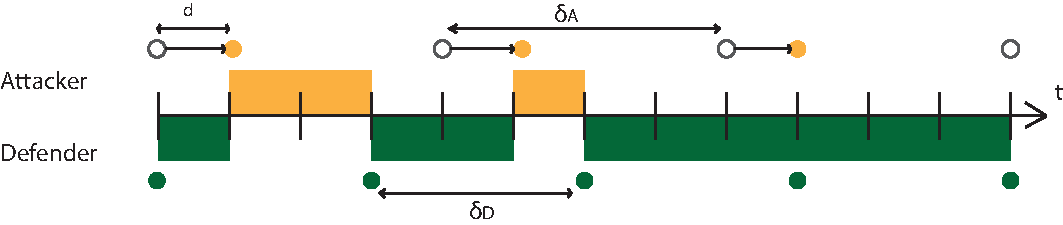
\includegraphics[scale=0.7]{Images/DefFlip.pdf}
\caption{Formalization of a FlipIt game with delay: A representation of a FlipIt game where both players are playing periodically. Every move or flip is indicated by a green or orange circle, respectively dark gray and light grey.  The defender is represented in green (dark grey) and plays with a period of $\delta_{D}$. The flip of the attacker is represented by a white circle, but because there is a delay d, the attacker only controls the resource after time d represented by an orange circle (light grey). The attacker plays with a period of $\delta_{A}$. The green and orange rectangles represent the amount of time the respective player is in control of the resource.}
\label{FlipItDelay}
\end{figure}

\begin{description}
\item $i$: Denotes the player. \textit{D} denotes the defender, and \textit{A} denotes the attacker which differs form the notation in \citep{FlipIt}, where the defender is denoted by the subscript \textit{0} and the attacker by the subscript \textit{1}.
\item $\delta_{i}$: The length of the interval between two consecutive moves of player \textit{i}. 
\item $\alpha_{i}$: The average flip rate of player \textit{i}, given by $\alpha_{i}=1/\delta_{i}$.
\item $k_{i}$: The cost of player \textit{i}'s moves.
\item $d$: The delay caused by the virus propagation.
\item $G_{i}(t)$: The total gain of player \textit{i}, which is the amount of time player \textit{i} is in control over the resource up to time \textit{t}.
\item $\gamma_{i}$: The average gain rate of player \textit{i}, defined as $G_{i}(t)/t$
\item $\beta_{i}$:  The average benefit rate up to time \textit{t}, defined as  $\beta_{i} = \gamma_{i} -k_{i} \alpha_{i} $.
\item $opt_{i}$: The optimum function for player \textit{i}. 
\end{description}

The adaptation of the FlipIt model starts from the assumption that, when an attacker attacks at time \textit{t}, he doesn't get immediate control over the resource, but he only gains control at time \textit{t + d}, with $d$ denoting the time needed to infect a sufficient number of (or all) nodes. If the defender flips the network before the period $d$ has elapsed (so, somewhere between $t$ and $t + d$), then the attacker will never gain full control over the resource. (See figure \ref{dt} at point 3 and 4). This implies that the mathematical formulas for gain and benefit need to be adapted to the fact that the attacker loses part of his benefit because of this delay. In the remainder of this paper, we will adapt the formalization of the FlipIt game using the delay variable $d$. \\ 

\begin{figure}[hbtp]
\centering
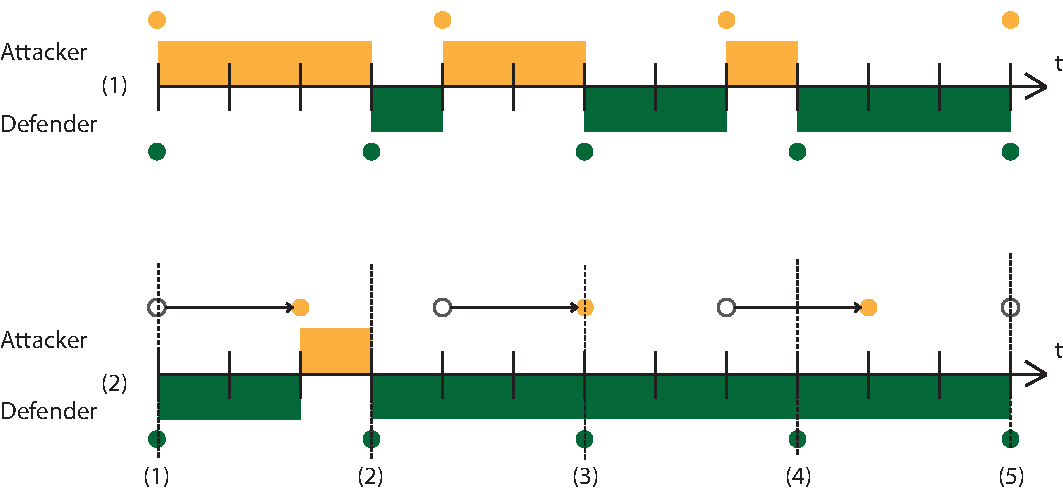
\includegraphics[scale=0.7]{Images/Delayuitgelegd.pdf}
\caption{The first game is the basic FlipIt game. The second is the FlipIt game with a delay. During the first flip of the attacker, the defender moves after the delay, causing the attacker to get control over the resource. During the second flip of the attacker, the defender flips at time t+d, causing the defender to take control over the resource before the attacker. During the third and final flip of the attacker, the defender flips during time t+d, causing the attacker to never gain control over the resource. }
\label{dt}
\end{figure}

Similarly as in \cite{FlipIt}, we split the formalization in two cases. In the first case the defender plays at least as fast as the attacker, in the second case the attacker plays at least as fast as the defender. For each of these cases, the benefit formula of the basic case without delay is presented first, and subsequently the delay is introduced.  \\

Intuitively, we could assume that $d$ can never be bigger than $\delta_{A}$ because then the attacker would play again before the delay has finished. This would seemingly result in a gain for the defender that is always 1, but this is not always true. Assume for example that an attacker plays with an interval of 3 time units, that the delay is equal to 4 time units and that the defender only plays every 8 time units. This situation is represented in figure \ref{langedelay}. Since the delay is shorter than the period of the defender, the attacker takes control of the resource once the delay has elapsed, until the defender plays. However, if the delay is larger that the period of the defender, then the defender will always be in control. This situation is represented in figure \ref{langeredelay}, where the attacker plays with an interval of 5 time units, the delay is equal to 6 time units and the defender plays with an interval of 4 time units. From this we can conclude that it only makes sense to calculate the formulas for the cases where $d$ is smaller than $\delta_{D}$. We can already conclude that it is of no use for the attacker to play when the delay is bigger than $\delta_{D}$. 




\begin{figure}[hbtp]
\centering
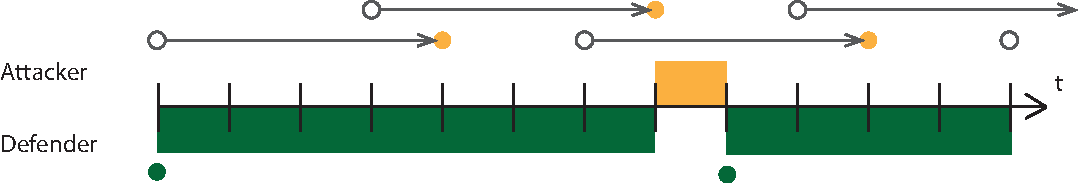
\includegraphics[scale=0.7]{Images/FlipItCase1delay.pdf} 
\caption{FlipIt with delay propagation where $\delta_{D} > d > \delta_{A}$.   }
\label{langedelay}
\end{figure}

\begin{figure}[hbtp]
\centering
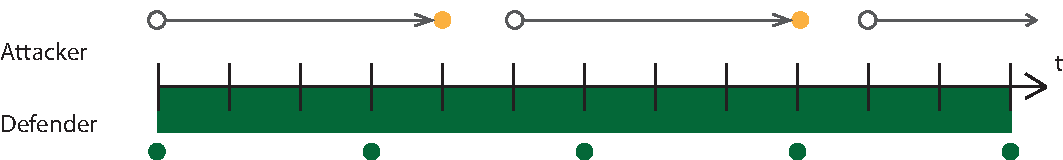
\includegraphics[scale=0.7]{Images/FlipItCase1delaytobig.pdf} 
\caption{FlipIt with delay propagation where $ d > \delta_{D}$ }
\label{langeredelay}
\end{figure}


In the original model of FlipIt \cite{FlipIt}, the authors express the formulas in terms of $\alpha_{D}$ and $\alpha_{A}$. However, when introducing the delay, some formulas become much simpler when expressed in terms of $\delta_{D}$ and $\delta_{A}$. Therefore in the remainder of this paper, we will formulate the model using both $\alpha_{i}$ and $\delta_{i}$, depending on which variable gives the simplest representation of the formulas.

\subsection*{\textbf{Case 1:} $\delta_{D} \leq \delta_{A} $ (The defender plays at least as fast as the attacker.) }

Let $r = \dfrac{\delta_{D}}{ \delta_{A} }$. The intervals between two consecutive defender's moves have length $\delta_{D}$. Consider a given defender move interval. The probability over the attacker's phase selection that the attacker moves in this interval is r. Given that the attacker moves within the interval, he moves exactly once within the interval (since $\delta_{D} \leq \delta_{A} $) and his move is distributed uniformly at random within this interval. \\

The expected period of attacker control within the interval as the moment on which the attacker gains control is uniformly distributed over the defender's interval. On average the attacker will gain control at time r/2. So the expected gain is equal to the remainder of the defender interval, i.e. r/2, without considering the delay by a virus. Therefore the benefit for the attacker, without considering the delay, can be expressed as follows:

\begin{equation*}
\beta_{A}(\delta_{D},\delta_{A}) =\dfrac {r} {2} - k_{A} \alpha_{A} = \dfrac {\delta_{D}} {2\delta_{A}} - k_{A} \alpha_{A}  
\end{equation*}\\

Correspondingly, the benefit for the defender can be expressed as:
\begin{equation*}
\beta_{D}(\delta_{D},\delta_{A}) =1 -  \dfrac {r} {2} - k_{D} \alpha_{D} = 1 - \dfrac {\delta_{D}} {2\delta_{A}} - k_{D} \alpha_{D} 
\end{equation*}

\begin{figure}[hbtp]
\centering
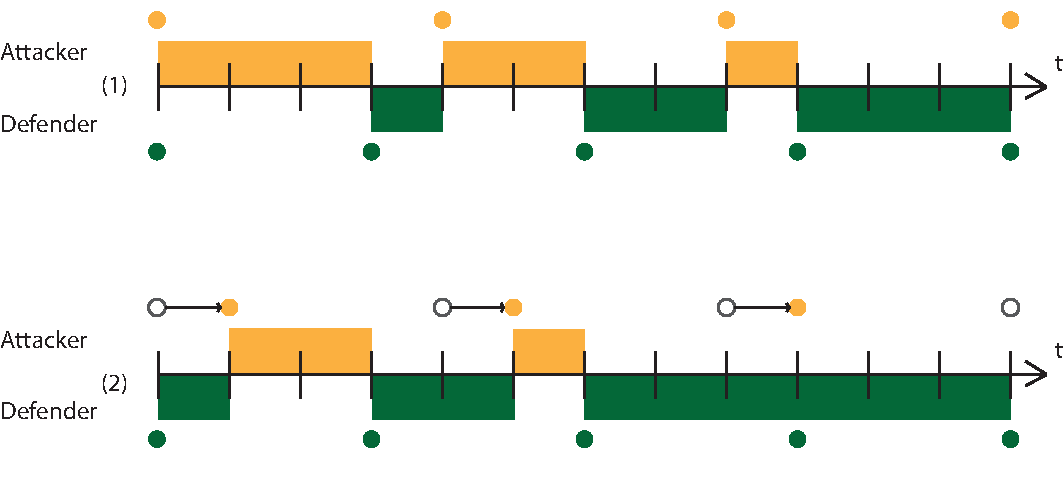
\includegraphics[scale=0.7]{../../doc/template/Images/DiffDelayCase1.pdf}
\caption{Case 1: Difference between a basic FlipIt game and a FlipIt game with a delay. Case (1) is the FlipIt game without a propagation delay and case (2) is with a propagation delay. The delay is denoted with an arrow. The attacker is only in control when the circle becomes orange (light grey).}
\label{fig:delaycase1}
\end{figure}




However, because of the delay required for virus propagation, the maximal time of control is reduced to $\delta_{D}-d$ , see figure \ref{fig:delaycase1}. While the probability that the attacker will move in the interval of the defender is still \textit{r}, the gain will not be half of the interval. Indeed, if the attacker plays after $\delta_{D}-d$, given the delay \textit{d}, he will never gain control in that interval (see figure \ref{tijdens interval}). 
\begin{figure}[hbtp]
\centering
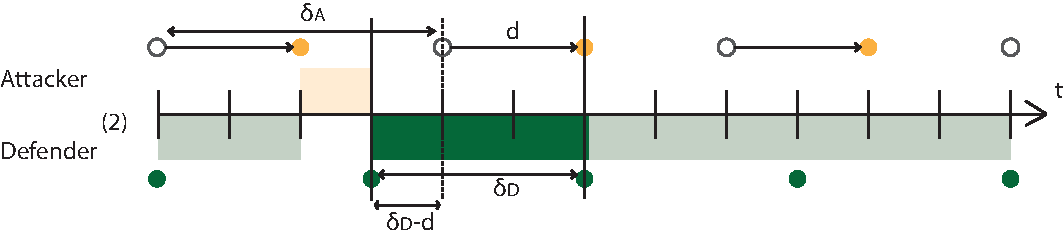
\includegraphics[scale=0.7]{../../doc/template/Images/delaydtijdens.pdf}
\caption{Attacker playing to late. If the attacker enters the defender's interval after $\delta_{D} -d$, he can not get in control in that interval.}
\label{tijdens interval}
\end{figure}The probability that the attacker plays early enough is $\dfrac{\delta_{D}-d}{\delta_{D}}$, giving the attacker an average gain of $\dfrac{\delta_{D}-d}{2}$ (the average remainder of the defender interval after the attacker flipped). If the attacker moves after the period of $\delta_{D}-d$, the gain of the attacker will be zero. The probability that this happens is  $\dfrac{d}{\delta_{D}}$. Looking at one interval of the defender, the average gain rate of the attacker can thus be expressed as follows:


\begin{equation*}
\gamma_{A}(\delta_{D},\delta_{A}) = \dfrac {1}{\delta_{D}} [ \dfrac{\delta_{D}}{\delta_{A}} \cdot \big[ \dfrac{\delta_{D}-d}{\delta_{D}} \cdot \dfrac{\delta_{D}-d}{2} + \dfrac{d}{\delta_{D}} \cdot 0 \big] ]
\end{equation*}
As the formula above is valid for each defender interval, the average gain rate over the entire game is:
\begin{equation*}
\gamma_{A}(\delta_{D},\delta_{A}) = \dfrac{(\delta_{D} -d)^{2}}{2\delta_{D}\delta_{A}}
\end{equation*}

To find the benefit, the cost of moving is subtracted from the average gain. 
\begin{equation}
\beta_{A}(\delta_{D},\delta_{A}) = \dfrac { (\delta_{D}-d) ^{2}} {2 \delta_{D}  \delta_{A}} - \dfrac{k_{A}}{\delta_{A}}
\label{Benfcase1:attacker}
\end{equation}

 
 The benefit of the defender is then as follows:
\begin{equation}
\beta_{D}(\delta_{D},\delta_{A}) = 1 - \dfrac { (\delta_{D}-d) ^{2}} {2 \cdot \delta_{D}  \delta_{A}} - \dfrac{k_{D}}{ \delta_{D}}
\label{Benfcase1:defender}
\end{equation}
~~\\
For this case where $d$=0, we this equals the formula of the original FlipIt game \citep{FlipIt} [p675].\\





\subsection*{\textbf{Case 2:} $\delta_{A} \leq \delta_{D} $ (The attacker plays at least as fast as the defender.) }

First let $r = \dfrac{\delta_{D}}{ \delta_{A} }$. The intervals between two consecutive attacker's moves have length $\delta_{A}$. Consider a given attackers move interval. The probability over the attacker's phase selection that the defender moves in this interval is $\dfrac{\delta_{A}}{ \delta_{D} } = (1/r)$. Given that the defender moves within the interval of the attacker, he moves exactly once within this interval (since $\delta_{A} \leq \delta_{D} $) and his move is distributed uniformly at random. \\

A similar analysis as in case 1 for a FlipIt game without a propagation delay yields the following benefits:

\begin{equation*}
\beta_{D}(\delta_{D},\delta_{A}) = \dfrac {1} {2r} - k_{D} \alpha_{D} = \dfrac {\delta_{A}} {2\delta_{D}} - \dfrac{k_{D} }{\delta_{D}} 
\end{equation*}
\begin{equation*}
\beta_{A}(\delta_{D},\delta_{A}) =1 - \dfrac {1} {2r} - k_{A} \alpha_{A} = 1- \dfrac {\delta_{A}} {2\delta_{D}} - \dfrac{k_{A}}{ \delta_{A}}  
\end{equation*}\\

An intuitive solution for the case with a virus would be to subtract the benefit of the attacker received in each interval with the delay similarly as in case 1. This would yield the following formula:
\begin{equation*}
\beta_{A}(\delta_{D},\delta_{A})=\dfrac{(\delta_{A} - d)^2}{2\delta_{A}\delta_{D}} - \dfrac{k_{D}}{\delta_{A}}
\end{equation*}

This however results in an overestimation. 
%By simulation the game, it can be notices that the closer $\delta_{A}/\delta_{D}$ is equal to one, the better the approximation. If $\delta_{A}/\delta_{D} = 1$ the result is correct. 
The reason this formula overestimates the benefit of the attacker is that it assumes that the defender is always in control during the delay. However, if the attacker was in control in the previous interval, then he continuous to be in control during the period of the delay, see figure \ref{fig:case2}. This means that the average benefit formulas for this case cannot be derived from one interval only; what happens in the previous interval must be taken into account. \\

We know that the defender's moves are instantaneous. Therefore, it is easier to calculate the benefit of the defender. Because the defender moves slower than the attacker we know that if the defender moves during the interval of the attacker, he only moves once within this interval.

The defender will move during the interval of the attacker with a probability of $\dfrac{\delta_{A}}{\delta_{D}} $. If this happens, the defender will be in control for the remainder of this interval. In the next interval the attacker will have to regain control, meaning that during the delay, the defender stays in control, see figure \ref{fig:case2} cases (1) to (4). The defender will keep the control over the resource in the next interval over a period of the delay, namely \textit{d}. \\

Consider a timespan $\delta_{A} + d$, representing the attacker's interval followed by the delay period in his next interval. If we assume that $\delta_{A}+d<\delta_{D}$, we can infer that the defender will never move twice during this timespan.
Because $d + \delta_{A} \leq \delta_{D}$ the next move of the defender in this second interval will never occur during the delay, meaning that the entire delay can be considered as an extra benefit resulting of a play in the previous interval. 
So, every time the defender plays, he will get an average gain of $\dfrac{\delta_{A}}{2}$ in the interval where he plays and in the next interval will always receive a extra gain of $d$, yielding a total average gain per interval of
$\dfrac{(d+\dfrac{\delta_{A}}{2})}{\delta_{A}}$

For the case with a delay we consider two cases, Case a and Case b, depending on whether the delay is shorter or longer than the difference between the attacker's and the defender's period.  \\

\begin{figure}[hbtp]
\centering
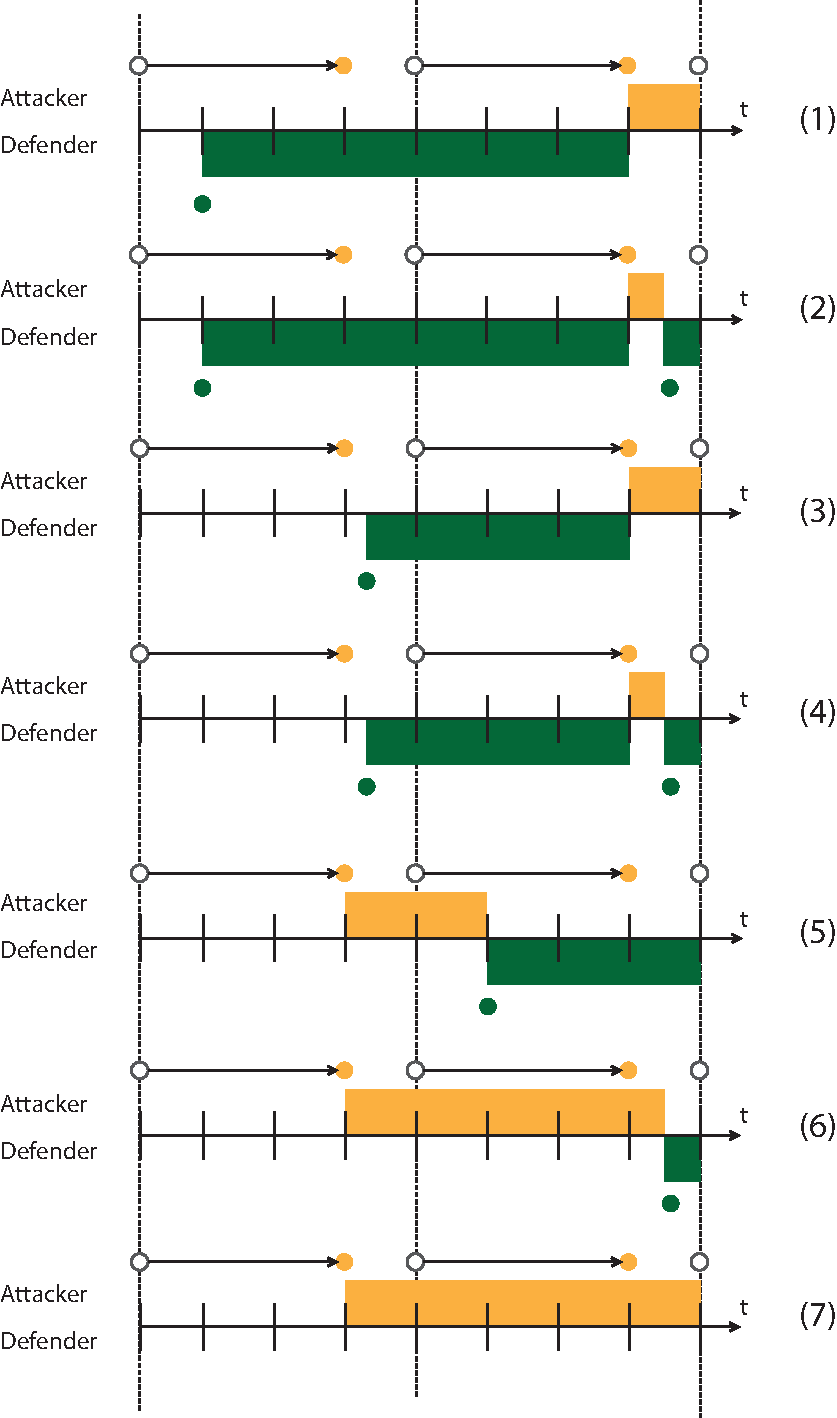
\includegraphics[scale=0.7]{../../doc/template/Images/FlipIt2.pdf}
\caption{All possible cases for the attacker and the defender in Case 2.A where $d + \delta_{A} < \delta_{D}$. As can be seen in cases (1) to (4), the defender will have control during a period of \textit{d} over the resource in the next interval when the defender has flipped in the previous interval.}
\label{fig:case2}
\end{figure}

\subsubsection*{\textbf{Case 2.a:} $ \delta_{D} \geq d + \delta_{A} \geq \delta_{A}$}
%The first case is where the defender's period is larger than the sum of the delay and the attacker's period. 
In this case the delay will never be counted twice in the defender's  benefit formula. To determine the total gain rate of the defender we need to know the probability that the defender will move during an interval and what the average time is that the defender controls the resource. Given that if the defender moves he will always benefit entirely from a period of delay in the next interval of the attacker, his total gain is $\dfrac{(d+\dfrac{\delta_{A}}{2})}{\delta_{A}}$ in one interval (as previously calculated. The total gain  rate of the defender is then the probability that the defender will move during an interval of the attacker multiplied by the total average gain per interval: 

\begin{equation*}\label{first}
\gamma_{D}(\delta_{D},\delta_{A}) = \dfrac{\delta_{A}}{\delta_{D}} \cdot \dfrac{(d+\dfrac{\delta_{A}}{2})}{\delta_{A}} 
\end{equation*}
\begin{equation*}\label{first}
\gamma_{D}(\delta_{D},\delta_{A}) = \dfrac{\delta_{A}}{2\delta_{D}} + \dfrac{d}{\delta_{D}} 
\end{equation*}\\
This yields the following benefit formula:
\begin{equation}\label{benfcase2a:defender}
\beta_{D}(\delta_{D},\delta_{A}) = \dfrac{\delta_{A}}{2\delta_{D}} + \dfrac{d}{\delta_{D}} - \dfrac{k_{D}}{ \delta_{D}}
\end{equation}\\

The benefit for the attacker will be as follows:
\begin{equation}\label{benfcase2a:attacker}
\beta_{A}(\delta_{D},\delta_{A}) = 1 -\dfrac{\delta_{A}}{2\delta_{D}} - \dfrac{d}{\delta_{D}} - \dfrac{k_{A}}{ \delta_{A}}
\end{equation}\\



It is crucial that $ \delta_{D}$ is at least as large as $d + \delta_{A}$. If not, the defender can move during the delay in the interval following the interval in which the defender already moved. This would result in an overlap between the average gain of $\dfrac{\delta_{A}}{2} +d$ and the delay. The above benefit formula would then include to much gain for the defender: the potential overlap during the delay would be counted twice. See figure \ref{countedtwice}\\

\begin{figure}[hbtp]
\centering
\caption{Cases where the delay would be counted twice.}
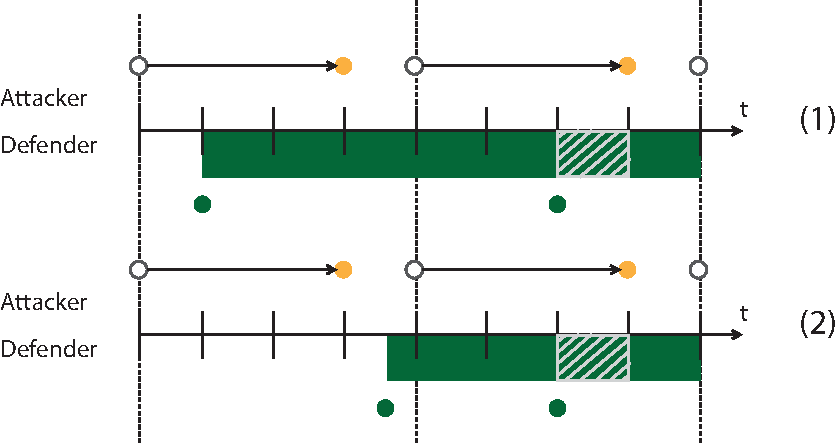
\includegraphics[scale=0.7]{Images/flipcase2nb.pdf}
\label{countedtwice}
\end{figure}

~~ \\
\subsubsection*{\textbf{Case 2.b:} $d + \delta_{A} \geq \delta_{D} \geq \delta_{A}$}
~~~\\

To obtain the formula in case of a too long delay, we therefore need to subtract this overlapping gain from the above formula. 
Since $\delta_{D} \geq \delta_{A}$, if the defender enters the interval immediately after the attacker has played, the defender cannot have played in the previous interval. In that case, there is no overlap. So the problem of the overlap only appears if the defenders enters late enough and thus only the last part of the delay is subject to overlap. The larger the difference between the interval of the defender and the attacker, the smaller the risk of overlap. Concretely, only the last part of length $d - (\delta_{D} - \delta_{A})$ is subject to overlap. Hence, the probability of overlap is $\dfrac{ d - (\delta_{D} - \delta_{A})}{\delta_{D}}$ and the average gain will be half of this interval:  $\dfrac{ d - (\delta_{D} - \delta_{A})}{2}$.  The gain rate to be subtracted is therefore:\\

\begin{equation*}
\dfrac{1} {\delta_{A}} \cdot \dfrac{d - (\delta_{D} - \delta_{A})}{\delta_{D}} \cdot \dfrac{d - (\delta_{D} - \delta_{A})}{2}
\end{equation*}

The total gain rate for the defender is obtained by subtracting this term from the gain rate of case a:
 \begin{equation*}
\gamma_{D}(\delta_{D},\delta_{A}) = \dfrac{\delta_{A}}{\delta_{D}} \cdot \dfrac{(d+\dfrac{\delta_{A}}{2})}{\delta_{A}} - \dfrac{(d - (\delta_{D} - \delta_{A}))^{2}}{2 \delta_{D} \delta_{A}}
\end{equation*}
\begin{equation*}
\gamma_{D}(\delta_{D},\delta_{A}) = \dfrac{\delta_{A}}{2\delta_{D}} + \dfrac{d}{\delta_{D}} - \dfrac{(d - (\delta_{D} - \delta_{A}))^{2}}{2 \delta_{D} \delta_{A}}
\end{equation*}\\
This yields in the following benefit formula:
\begin{equation}\label{benfcase2b:defender}
\beta_{D}(\delta_{D},\delta_{A}) = \dfrac{\delta_{A}}{2\delta_{D}} + \dfrac{d}{\delta_{D}} - \dfrac{k_{D}}{ \delta_{D}} - \dfrac{(d - (\delta_{D} - \delta_{A}))^{2}}{2 \delta_{D} \delta_{A}}
\end{equation}\\
 
Consequently, the benefit for the attacker will be:
\begin{equation}\label{benfcase2b:attacker}
\beta_{A}(\delta_{D},\delta_{A}) = 1 -\dfrac{\delta_{A}}{2\delta_{D}} - \dfrac{d}{\delta_{D}} - \dfrac{k_{A}}{ \delta_{A}} + \dfrac{(d - (\delta_{D} - \delta_{A}))^{2}}{2 \delta_{D} \delta_{A}}
\end{equation}\\

%~~\\
%\subsection{Conclusion of this chapter}
%\begin{description}
%\item[-]
%\item[-]
%\item[-]
%\end{description}
% ... en zo verder tot
%\chapter{The Final Chapter}
\label{cha:n}


\section{chap}

%%% Local Variables: 
%%% mode: latex
%%% TeX-master: "thesis"
%%% End: 

\chapter{Conclusion}
\label{chapter5:conclusion}

This paper presents an adaptation to the basic FlipIt game by \citep{FlipIt} to model an attacker with a delay.  We list a set of extensions that might be interesting for further research.
\section{Further work}

\begin{description}
\item \textit{Nash equilibria}\\ This paper concluded with the best responds functions of the attacker and the defender. The next step would be to calculate the Nash equilibria. For these calculation multiple cases have to be examined. All the possible cases regarding $k_{A}, k_{D}$ and $d$. 
\item \textit{Analysing other renewal strategies} \\ By analysing other renewal strategies, it might be interesting to find out if the original result regarding periodic and renewal strategies of the basic FlipIt game still stands. This result was that periodic strategies strongly dominate the other renewal strategies if an opponent plays with a non-adaptive strategy. 
\item \textit{Delay for the defender}\\ This paper only assumed that the attacker had a delay. It could be interesting to have a defender with a delay. This situation could happen when it takes some time to make a patch a system or when a new exploit is found. 
\item \textit{Variable delay} \\This paper assumed that the propagation delay had a fixed value. This can be relaxed by giving the attacker a delay that can vary every flip. The delay is always negative for the attacker, so the attacker will always choose the lowest delay. But if the attacker always sends a new worm at every flip, it could be that the delays vary. So a variable delay would be more accurate to simulate a real world case. 
\item \textit{The defender flips a subset of nodes} \\ Our model assumes that if the defender flips, he flips the whole network. An option for the defender would be to flip a subset of nodes in the network. If the costs of the flipping are related to the amount of nodes that are flipped, this option might be interesting to look at. It could be that a certain subset of nodes is found that protects the whole network. The PageRank matrix explained in Chapter 5 can help with finding the right nodes. \\

\end{description}


\section{General results and conclusions}
Our FlipIt model with worm propagation delay showed us some interesting results. 
\begin{itemize}
\item When the defender plays faster than the delay, the attacker will either have a negative benefit or a benefit equal to zero if the flips do not cost anything. It is for the defender a target to be able to play at a rate smaller or equal to the delay.
\item If the defender can play with a cost equal to zero, the attacker will not play. The defender can play at any rate he wants, and the attacker is always disadvantaged by his delay.
\item From a certain value for the speed of the attacker, the defender will not play any more or will play at the same rate. The same for the attacker.
\end{itemize}

As of today APTs become more and more extraordinary pieces of malicious code. There are APTs known to survive military-grade disk wiping and reformatting, and even after the reformatting and reinstalling the operating system are able to send sensitive data (Equation group \citep{Equation}). This means that even if you know that an APT is on your network, the actual practical "flip" has to exist or known by the defender.  \\
The best way to secure a system is to find the weakest link. This is mostly the employee. To counter this problem, you have to raise the awareness of the risks.  Awareness is very important. Even if you have good security protection layers, spam filters, firewalls, a phishing mail opened by one of your employees or a USB stick is enough to infect a pc on the network and by that it can spread further. But a system can never be 100\% waterproof. If an infection has occurred and the defender knows a counter measure, the FlipIt game will help to prevent a system to be compromised. 
%%% Local Variables: 
%%% mode: latex
%%% TeX-master: "thesis"
%%% End: 


% Indien er bijlagen zijn:
%\appendixpage*          % indien gewenst
%\appendix
%\chapter{The First Appendix}
\label{app:A}
\includepdf[pages=-]{paper.pdf}


%%% Local Variables: 
%%% mode: latex
%%% TeX-master: "thesis"
%%% End: 

% ... en zo verder tot
%\chapter{The Last Appendix}
\label{app:n}
\includepdf[pages=-]{finaal.pdf}


%%% Local Variables: 
%%% mode: latex
%%% TeX-master: "thesis"
%%% End: 


\backmatter
% Na de bijlagen plaatst men nog de bibliografie.
% Je kan de  standaard "abbrv" bibliografiestijl vervangen door een andere. plainnat
\bibliographystyle{abbrv}
\bibliography{reffiess}

\end{document}

%%% Local Variables: 
%%% mode: latex
%%% TeX-master: t
%%% End: 

%@Misc{Coursera,
%author = {Coursera},
%title = {Game Theory by Matthew O. Jackson, Kevin Leyton-Brown, Yoav Shoham},
%howpublished = {https://class.coursera.org/gametheory-004}, last checked on 2015-02-22}
%}
%
%
%@Misc{Symantec,
%author = {Symentec},
%title = {2014 Internet Security Threat Report, Volume 19},
%howpublished = {http://www.symantec.com/content/en/us/enterprise/other-resources/b-istr-appendices-v19-221284438.en-us.pdf}, last checked on 2015-02-22}
%}